% !TeX root = ./thesis.tex

% Package importing
\documentclass[12pt, a4paper, oneside]{article}
\usepackage[utf8]{inputenc}
\usepackage[T1]{fontenc}    % Use 8-bit T1 fonts
\usepackage{setspace}
\usepackage[english]{babel} % Set English as main language
\usepackage[utf8]{inputenc} % Allow utf-8 input
\usepackage{mathptmx}
\usepackage{amsfonts}       % Blackboard math symbols
\usepackage{amsmath}        % AMS Math
\usepackage{amssymb}        % AMS Symbols
\usepackage{booktabs}       % Professional-quality tables
\usepackage{threeparttable}
\usepackage{enumitem,kantlipsum}
\usepackage{caption}        % Captions
\usepackage{float}          % Float control
\usepackage{geometry}       % Easily define margins
\usepackage{graphicx}       % Graphic materials (e.g., images)
\usepackage{hyperref}       % Hyperlinks
\usepackage{microtype}      % Microtypography
\usepackage{rotating}       % Allow page rotation (e.g., for large table)
\usepackage{tikz}           % Drawings
\usepackage{url}            % Simple URL typesetting
\usepackage{setspace}
\usepackage{subfig}
\usepackage{graphicx}
\usepackage{titlesec}
\usepackage{fancyhdr}
\usepackage{adjustbox}
\usepackage{pdflscape}
\usepackage{multirow}
\usepackage{array}
\usepackage[nopar]{lipsum}
\usepackage[style=apa, backend=biber]{biblatex}
\geometry{paper=a4paper, % Change to letterpaper for US letter
right=2.54cm, % Inner margin
left=2.54cm, % Outer margin
bindingoffset=.5cm, % Binding offset
top=2.54cm, % Top margin
bottom=2.54cm, % Bottom margin
}

\pagestyle{fancy}
\fancyhf{}
% \rhead{\footnotesize\textsc{Master Thesis}}
% \lhead{\footnotesize Does European Central Bank Tone Embedded In Speeches Move Asset Prices?}

\lhead{\leftmark}
\rhead{\thepage}
% Adding bib file
\addbibresource{zotero.bib}
\pagenumbering{arabic}
% Removing indents before paragraphs
\setlength\parindent{0pt}
\usepackage{setspace}
\onehalfspacing

% Custom function for creating equation conditions
\newenvironment{conditions}
  {\par\vspace{\abovedisplayskip}\noindent\begin{tabular}{>{$}l<{$} @{${}={}$} l}}
  {\end{tabular}\par\vspace{\belowdisplayskip}}

% Start of document
\begin{document}
\doublespacing

%Titlepage in titlepage.tex
\begin{titlepage}
    \begin{center}
        \vspace*{0.5cm}
        \textsc{\large Master Thesis}
        \vspace{0.5cm}
        \hrule
        \vspace{0.4cm}
        \huge{\bfseries Does European Central Bank Tone Embedded In Speeches Move Asset Prices?}
        \vspace{0.5cm} 
        \hrule
        \vspace{1.5cm} 
        \begin{minipage}[t]{7cm}
            \flushleft \large
                \emph{Student:}

                {Indrė \textsc{Butaitė}}

                (i6155833)

        \end{minipage}
        \hfill
        \begin{minipage}[t]{7cm}
            \flushright \large
                \emph{Supervisor:}

                {Dirk \textsc{Broeders}}
        \end{minipage}
        % \vspace{0cm}
        \vfill
        
\includegraphics[width=2.5cm]{resources/University_Crest.png}
        \vspace{1cm}
        \vfill
        \large
            Maastricht University

            School of Buiness and Economics

            \vspace{2cm}

            Thesis submitted for the degree of

            \emph{M.Sc. Financial Economics (Asset Pricing)}
        \vspace{1.5cm}
        \vfill
        {\large \today}


    \end{center}
\end{titlepage} 
%Abstract
\newpage
\begin{abstract}
    hello
\end{abstract}


\newpage
\tableofcontents
\listoffigures
\listoftables
\newpage
\parskip=\baselineskip
\titlespacing\section{0pt}{12pt plus 4pt minus 2pt}{-12pt plus 2pt minus 2pt}
\titlespacing\subsection{0pt}{0pt plus 4pt minus 2pt}{-12pt plus 2pt minus 2pt}
\titlespacing\subsubsection{0pt}{12pt plus 4pt minus 2pt}{-12pt plus 2pt minus 2pt}
\section{Introduction}
%\lipsum[2]
%\lipsum[3]


%Transparency index


\textbf{\textit{Research Question: How do asset prices react to monetary policy and economic outlook sentiment in European Central Bank speeches?}}


In this paper I will answer the following questions: 
\begin{enumerate}
  \item How do Euro area bonds of different maturities 3 months 1-, 2-, 5-, 7-, 10-, 20- and 30 years react to sentiment in ECB’s speeches?
  \item How do stock returns react to sentiment in ECB’s speeches?
  \item How does the credit spread between Italian and German sovereign bonds react to sentiment in ECB’s speeches?
  \item How do inflation expectations react to sentiment in ECB’s speeches?
  \item How do asset prices react to sentiment in speeches by ECB representatives of different ranks? (e.g. president, vice-president and board members)
\end{enumerate}
\section{ECB's Communication Overview}

\subsection{Why ECB's Communication Matters?}
The primary objective of the ECB is to maintain price stability. The main tool to achieve this is by manipulating short-term overnight interest rates. However, the ECB understands that market agents do not make decisions based on these short-term interest rates. Instead, what matters is the ECB's signals to the market via alteration of these rates. These signals affect market expectations regarding the future path of short-term interest rates, which then impact long-term interest rates as shown by expectations hypothesis of the term structure of interest rates in Equation \ref{eq:expect} (\cite{blinder2008}).

\begin{equation}
    \label{eq:expect}
    R_{t} = \alpha_{n} + (1/n)(r_{t} + r_{t+1}^{e} + r_{t+2}^{e} + \dots + r_{t+n-1}^{e}) + \varepsilon_{1,t}
\end{equation}

\vspace{-16pt}

where $R_{t}$ is long-term interest rate, $r_{t}$ is current short-term interest rate of $n-1$ days in the future and $\alpha_{n}$ is the term premium, assumed to be stochastic ($\varepsilon_{t}$). Long-term interest rates matter because they influence private agents' investment decisions, which drive the economy. 

Since the financial crisis, the overnight rate is stuck near zero. Therefore the ECB introduced unconventional monetary policy tools and intensified its communication efforts to deliver its signals. With its communication, the ECB sends signals about the future short-term interest rates, and through these rates, it can influence the long-term rates as seen in Equation \ref{eq:expect}. This form of communication is called "forward guidance".
 

If agents are rational and are fully aware of the economic conditions and the ECB's reactions to them, the ECB's communication would be redundant (\cite{woodford2005}). Agents would not react to the signals of the ECB as they already incorporated them into their expectations once the new information came out. However, in reality ECB's communication matters for several reasons. First, the ECB updates its economic model. It incorporates new parameters, updates its policy strategy, etc.,  which take time for the market agents to learn about. Second, agents sometimes may act irrational. Third, the ECB specialises in analysing the economy, therefore it may have more and better knowledge. In addition, the ECB's communication becomes especially important during recessions as crises can make it difficult for the market agents to interpret the information and anticipate monetary policy responses (\cite{coenen2017}). For all these reasons above it is evident that the ECB's communication has an influence on agents behaviour and hence the economy. 

Recognizing this influence, the ECB continuously aims to improve how it conducts its communication as it is of the utmost importance that the market participants correctly understand the ECB's signals. The ECB notes on its website: "how people spend and invest today, and expect the economy to develop tomorrow, can affect our job of keeping prices stable" (\cite{europeancentralbank2021}). Therefore, the ECB continuously simplifies its communication, stresses its commitment to what it says, and increases its communication frequency to help people better understand its decisions and build trust. Today the ECB uses a large number of tools to communicate with the public. These are press releases, press conferences, the blog, monetary policy accounts, speeches, interviews, and listening events. 
%%%%%%%%%%%%%%%%%%%%%%%%%%%%%%%%%%%%%%%%%%%%%%%%%%%%

\subsection{The Informativeness in the Speeches vs. Other Means of the ECB's Communication}


One of the ECB's communication means that gained recent attention is speeches. The number of speeches over the years has been gradually increasing (see Figure \ref{fig:figcombo1}). The ECB uses speeches to explain its monetary policy decisions and address other topics related to central banking, the financial system, and the economy. Therefore, speeches do not necessarily contain new information but instead clarify the information delivered through other communication means, mainly press conferences. Press conferences provide the public with updated monetary policy decisions and economic outlook projections. Therefore, one may think of speeches as a complement to the press conferences. 

Unlike press conferences which are held every six weeks immediately after new monetary policy decisions, speeches are flexible in their timing. Also, in comparison to press conferences that represent the Governing Council's view as a whole, speeches are given by the members of the Executive Board and represent individual views of the speakers. Moreover, press conferences have a standardized format and language, whereas speeches do not follow strict guidelines. Other communication tools such as interviews, the blog, and listening events are primarily used for public relations; therefore, I will not address them further.  

The role of the press conferences as a monetary policy tool is well understood in practice and the academic literature. However, not many researchers have spent time analyzing speeches, given that they are significantly less structured than the monetary policy press conferences. Regardless, provided that the ECB's representatives go through the effort of giving these speeches, one expects them to align with the bank's overall objective - price stability through manipulating the interest rates. Therefore, it is interesting whether speeches contain unique signals to the market agents and hence can be declared as another monetary policy tool to manage market expectations like press conferences or is it just a public relations tool like the interviews. I test this empirically.  


\section{Literature Review}
My paper relates to two strands of literature on central bank communication: i) its impact on financial markets, and ii) its quantification through textual analysis. The academic literature investigating the impact of the ECB’s communication and especially speeches on financial markets is scarce. For this reason, to have sufficient evidence in constructing hypotheses I also include papers exploring communication of other central banks where needed.

\subsection{Central Bank Communication and Asset Prices}
There is substantial evidence that central bank communication moves asset prices, suggesting that the central bank communication conveys relevant information to market participants, i.e., it contains news. For example, see the evidence on interest rates for the ECB (\cite{ehrmann2007, schmeling2019, rosa2007,brand2010,rosa2011,lamla2011}), the FED (\cite{kohn2003,gurkaynak2004,lucca2009}), the Bank of England (\cite{reeves2007}), the central banks of Czech Republic, Hungary and Poland (\cite{rozkrut2007}), the central bank of New Zealand (\cite{guthrie2000}) and the Swedish central bank (\cite{andersson2006}). Also, several papers discovered that central banks’ communication can steer the interest rates in the intended direction, implying that the communication is a monetary policy tool that allows the central banks to manage the expectations of the market participants. For instance, \textcite{guthrie2000} found that following the Reserve Bank’s of New Zealand tightening announcements, interest rates of all maturities increased. They showed that this increase is not caused by the simultaneous changes in the open market operations. In the same vein, \textcite{rosa2007} investigated the ECB press conferences and discovered that when the ECB’s communication is dovish (hawkish), the interest rates decrease (increase). Some studies even showed that central bank communication has a more significant impact on the bond market than the changes in the policy rate (see, e.g., \cite{gurkaynak2004,rosa2011}). \textcite{gurkaynak2004} explained that the policy rate changes in the US and Eurozone are rarely a surprise. For this reason, the tone used to explain the monetary policy decisions is the primary driver of the financial markets because the tone reveals the information regarding the path of the future policy expectations. Precisely, through this channel, the central banks guide the private sector's expectations.

Most of the literature on central bank communication analyzed press conferences that are used to convey monetary policy decisions and the reasons behind them. The speeches of central banks, on the other hand, have been overlooked. \textcite{kohn2003} are the first that studied the impact of speeches on interest rates. They investigated the speeches of FED that took place between 1989 and 2003 but did not find any influence on the interest rates. The researchers argue that speeches are too noisy, as they are given about a broad spectrum of topics, and some may have little to do with monetary policy or the economic situation. Nevertheless, more recent papers investigating the speeches of the ECB and other central banks found a significant impact on interest rates (\cite{andersson2006,rozkrut2007,ehrmann2007}). Furthermore, \textcite{reeves2007} and \textcite{connolly2004} found somewhat significant results. Across the total sample, they found very little influence on the interest rates. However, several speeches appear to have a significant impact on the volatility of the interest rates. As \textcite{kohn2003} they argue that the inclusion of all the speeches in the dataset hides the effect of speeches that are deliberately designed to influence expectations. For this reason, I intend to augment this approach by performing a pre-selective filter based on keyword frequency per speech to exclude the less relevant speeches. In doing so, I hope to minimize the noise experienced by the researchers above. Moreover, speeches, among other communication tools of the ECB, have become more critical for the conduct of monetary policy in the current low-inflation environment (\cite{bernoth2020}). Therefore, based on the above mentioned arguments, I hypothesize that:

\textbf{Hypothesis 1a:} The tone of the ECB speeches has an impact on interest rates.\\
\textbf{Hypothesis 1b:} When the tone of the ECB speeches is dovish (hawkish) the interest rates decrease (increase).


Delving deeper into the ECB’s communication, the impact of speeches on different maturities of interest rates is a natural area to investigate next. The ECB’s communication has a more substantial impact on the interest rates with the shorter-term maturities. For example, \textcite{lamla2011} found that the tone in the ECB’s press conferences only affects the interest rates of 4-12 months. They argue that given a communication signal today, financial markets expect the ECB to alter interest rates the soonest four months later, but not earlier. This indicates that the ECB prepares the market well in advance for the changes in the policy rates. Similarly, \textcite{musard-gies2006} and \textcite{rosa2007} discovered that the short end of the yield curve specifically yields with maturities of 6 and 12 months, react the most to the tone of the ECB’s press conferences. On the other hand, \textcite{ehrmann2007} found that the tone of the ECB’s speeches affects the interest rates with maturities even up to five years. It seems intuitive that the ECB’s communication mainly impacts short-term interest rates. The ECB cannot provide meaningful policy intentions more than several years ahead because future monetary policy decisions depend on the future economic environment. Also, the longer the maturity of interest rates, the less control the ECB can exercise because longer-term interest rates depict exogenous factors such as global interest rate trends and changing term premia (\cite{lucca2009}). This leads to my following hypothesis to be tested:


\textbf{Hypothesis 1c:} The tone in the ECB’s speeches has a stronger impact on the short end of the yield curve than on the long end.


During the press conference meeting of 12 March 2020, the ECB President Christine Lagarde mentioned that it is not the ECB’s role to “close the spread” referring to the gap between Italian and German bond yields. Immediately after her statement, Italy’s bond yields rose from 117bps to 174 bps, whereas Germany’s bonds remained at -74bps, indicating a 35\% increase in the spread (\cite{leombroni2021}). It was the biggest single-day increase in Italian government bonds in a decade. The market interpreted that the ECB will no longer be the lender of the last resort to Italy, which triggered Italy’s bond market sell-off. Lagarde immediately corrected this perception and apologized for her “botched” communication (\cite{arnold2020}). Recent academic literature explored the role of the ECB’s communication on yield spreads. For example, \textcite{schmeling2019} found that the yield differential of BBB- and AAA-rated corporate bonds decreases (increases) when the tone in the press conferences of the ECB becomes more positive (negative). The researchers argue that the tone of the central bank communication influences the risk aversion of the market participants. For this reason, the default spread changes. \textcite{beaupain2020} also investigated the impact of the press conferences of the ECB on the yield spread. They provide supporting evidence that the ECB’s communication complements its actions in reducing the yield spread between the ten euro countries and Germany. The ECB’s communication was especially effective in reducing the yield spread for “distressed” countries such as Italy, Spain, Greece, Portugal, and Ireland. Following this, I am curious to explore whether the spread between Italian and German sovereign bonds changes due to sentiment in speeches. Therefore, based on the arguments above, my next hypotheses are accordingly:


\textbf{Hypothesis 2a:} The tone in the ECB’s speeches impacts the spread between Italian and German sovereign bonds.\\
\textbf{Hypothesis 2b:} When the tone is dovish (hawkish) the spread between Italian and German sovereign bonds decreases (increases).

In 2005 former ECB president Jeane-Claude Trichet in his speech, said, “I will argue that under some conditions the central bank can regain control of private expectations without necessarily changing interest rates, but by being visibly and credibly “alert”, explaining and stressing its commitment to maintaining inflation at levels consistent with the price stability objective” (\cite{europeancentralbank2005}). Unfortunately, very little research is done on the effects of the ECB’s communication on inflation expectations to support his statement. \textcite{ehrmann2007} are the first to investigate whether the inflation expectations react to the tone in the ECB’s speeches. However, they do not find any statistically significant results. The findings of \textcite{jansen2007}, to some extent, support Trichet’s statement. They found a significant relationship between the tone in press conferences and changes in break-even inflation but only during October and November 2005. The researchers argued that communication works in steering inflation expectations when the central bank credibly commits to a particular inflation goal, i.e. when the deeds support the communication. \textcite{ullrich2008} also provides somewhat supporting evidence to Trichet’s statement but again stresses the importance of credible commitment. She investigated the influence of the tone in the ECB’s press conferences on the inflation expectations of experts. She found that a hawkish tone, i.e., addressing the concern about inflation risks, induced financial market experts to adjust inflation expectations with a 6-month horizon upwards. This is caused by the experts’ disbelief in the ECB’s ability to act against this rising inflation in the upcoming six months. However, inflation expectations eventually adjust downward, as shown by \textcite{hubert2017}. He found that a hawkish tone in the ECB’s speeches has a negative effect on the long-horizon inflation expectations, but only if they are considered alone, without the ECB’s inflation projections. Following this, I aim to expand this scarce literature on inflation expectations by investigating the tone of the ECB’s speeches. I do not expect to find a strong relationship since the tone only indirectly impacts inflation expectations. My study is closest to \textcite{ehrmann2007}; however, given that a more recent study by \textcite{hubert2017} found somewhat significant results, my hypotheses are as follows:


\textbf{Hypothesis 3a:} The tone in the ECB’s speeches impacts inflation expectations.\\
\textbf{Hypothesis 3b:} When the tone is dovish (hawkish) there is an upward (downward) change in inflation expectations.


Besides the ECB’s communication impact on interest rates and inflation expectations, some studies also explored the relationship between the ECB’s communication and stock markets. For example, \textcite{ehrmann2007} found that when the ECB’s speeches carried tightening (loosening), monetary policy sentiment the Euro Stoxx 50 index decreased (increased). This is consistent with \textcite{schmeling2019} who investigated the tone in the press conferences of the ECB. \textcite{picault2017} also found that the Euro Stoxx 50 index reacts to the tone in the ECB’s press conferences. In addition, \textcite{apergis2019} explored the impact of ECB’s announcement wire news on the major international stock indexes, i.e., S\&P500, FTS100, CAC40, DAX, and Nikkei225. Specifically, when the tone in the ECB’s messages was positive, the stock returns were positive, whereas the volatility was negative and vice versa. \textcite{schmeling2019} explained that the positive sentiment surrounding monetary policy reduces peoples’ risk aversion resulting in higher willingness to invest in equity markets. For this reason, the stock prices increase. Following this I also aim to explore the relationship between the tone in the speeches and the stock market returns. Based on the evidence above I hypothesize:


\textbf{Hypothesis 4a:} The tone in the ECB’s speeches impact the stock returns.\\
\textbf{Hypothesis 4b:}  When the tone is  dovish (hawkish) the stock returns increase (decrease).

Thus far I looked at studies investigating the sentiment surrounding the monetary policy talk. However, a large portion of the ECB’s communication is also dedicated to provide the economic outlook prospects in the Eurozone. \textcite{ehrmann2007} is the only study that investigated the economic outlook tone of the ECB’s speeches. They discovered significant relationship between the economic outlook sentiment and financial assets such as Euro Stoxx 50 and short-term interest rates. However, no impact was found on inflation expectations. Similarly, \textcite{picault2017} explored the economic outlook tone embedded in ECB’s press conferences and found a significant impact on the stock market. Both papers found that a positive economic outlook tone led to an improvement in asset prices. I intend to expand this scarce literature on the economic outlook tone for the ECB’s speeches. Based on the evidence above, my hypotheses are accordingly:

\textbf{Hypothesis 5a:} The tone surrounding economic outlook in the ECB’s speeches matters for interest rates, credit spread, stock market, but not inflation expectations.\\
\textbf{Hypothesis 5b:} The positive (negative) economic outlook tone in the ECB’s speeches leads to an increase (decrease) in stock returns and decrease (increase) in interest rates and credit spread.


\textcite{ehrmann2007} assessed the communication strategies of the Fed and the ECB. They found that the US financial markets respond significantly more strongly to communication by Greenspan and less to statements by other FOMC members whereas Euro area markets react similarly to communication by the President and other Governing Council members. Unlike in the FED, the decision making in the ECB is collegial. For this reason, financial market agents react the same to the communication by the policy makers of different ranks in the Euro area. My obtained speech dataset is sorted into speeches by President, Vice-President and the remaining Board Members. Therefore, I also aim to explore whether my results support the findings of \textcite{ehrmann2007}. Given the evidence above, I hypothesize:


\textbf{Hypothesis 6:} Financial markets respond the same to the speeches by President, Vice-President and Board members.

%%%%%%%%%%%%%%%%%%%%%%%%%%%%%%%%%%%%%%%%%%%%%%%%%%%%%%%%%%%%%%%%%%%%%


\subsection{Quantifying Central Bank Communication}
Two main methods have been used in literature to quantify qualitative information. One is \textit{manual content analysis}, which involves reading a text, classifying it based on its content, and then coding it on a numerical scale. For example, \textcite{musard-gies2006} and \textcite{rosa2007} hand-coded the ECB’s press conferences based on the tone of the content into a grid-scale from -2 (very dovish) to +2 (very hawkish). Although manual classification is easy to carry out, it is labor-intensive and subjective. For instance, Rosa and Verga (in \cite{rosa2007}) disagreed on 22.58\% of classified statements.


More recent literature considered the drawbacks of manual content analysis and instead used an \textit{automated approach}. Specifically, a computer program is used to count how frequently certain words appear based on a pre-specified word list or dictionary. In dictionaries, words are allocated under specific topics and sentiments. For example, “unemployment” would be considered a negative word under the dictionary of \textcite{loughran2011}. If a text contains a lot of negative words like “unemployment” (other examples “uncertainty”, “crisis”, etc.) the text will likely convey a pessimistic message. Therefore, a central assumption is that the frequency of the words reflects the tone of the text. The score is then computed for example as the number of positive words minus the number of negative words scaled with total words in the text (see e.g., \cite{picault2017,baranowski2021}. The benefits of dictionaries are two-fold, convenience and robustness. Convenient because prebuilt lexicons are developed by NLP experts with certain classifications and/or types of source data in mind. If available, they are easily applied to one’s dataset and require relatively little programming for classification. Robust because the developers of most lexicons attempt to develop their lexicon so that it applies across as many datasets as possible without losing the predictive power of classifications.


\textcite{schmeling2019}, in their study, used \textcite{loughran2011}’s (LM) financial dictionary to quantify the press conferences of the ECB. They verify that the dictionary indeed captured how the ECB frames its macroeconomic fundamentals. \textcite{baranowski2021} also identified the LM dictionary as appropriate to measure the ECB’s monetary policy stance. However, \textcite{picault2017} are skeptical about the LM dictionary as it is a single-word dictionary and is not precisely designed for the ECB’s talk. The LM dictionary does not capture the monetary policy or the economic outlook sentiment specifically. It simply assigns words into either having positive or negative sentiment. Therefore, it may fail to capture the true ECB’s tone. However, if my speeches are too noisy to extract monetary policy or economic outlook sentiment as argued by \textcite{kohn2003}, then the LM dictionary is more appropriate as it derives a general tone of the communication – positive or negative. Given the discussion above, I intend to apply the LM dictionary to my speech dataset.


\textcite{baranowski2021} also identified \textcite{bennani2017}’s (BN) dictionary as another potential dictionary that correctly depicted the tone of the ECB’s communication. The BN dictionary is developed from the speeches of the members of the ECB’s Governing Council; therefore, the dictionary may closely reflect the context of my speech data set. However, the ECB’s speeches that I investigate are given only by the Executive Board members. Hence, there may be a mismatch in the structure and style of the communication between the BN dictionary and my speeches dataset. Also, the BN dictionary is a single-word dictionary. Therefore, there is a high chance of misclassifying certain words as it does not consider the context. Despite this, I believe the BN dictionary may be able to depict the tone in the ECB’s speeches to some extent. Therefore, I intend to apply it for robustness.


Finally, the most suitable to my speeches’ data is \textcite{picault2017}’s (PR) dictionary. The dictionary is constructed from the ECB’s press conferences and is divided into monetary policy and the economic outlook topics. In addition, the lexicon consists of a sequence of words, from 1-gram to 10-gram, where gram refers to a word. PR lexicon is likely to have only a small share of misclassifications because a sequence of 10 words can greatly capture the context of the text, at least much better than a single- or two-word dictionaries identified above. \textcite{picault2017} showed that its dictionary outperformed all of the above identified  dictionaries. However, the potential incompatibility between the PR-lexicon’s source data and the ECB's speech dataset used in this paper should not go unnoticed. Two possible limitations come to my mind, different types of speeches and different speakers. First, the PR-lexicon is based on the often structured and standardized ECB monetary policy decisions press conferences. In contrast, this paper’s dataset contains a broader array of speeches, some of which have little to do with monetary policy or economic outlook. Second, as the PR-lexicon was developed over the 2006-2014 timespan, the vocabulary was based on a smaller set of speakers. For example, given the switch in ECB presidents from Mario Draghi to Christine Lagarde, potential nuances in their different speech styles may be lost using the PR-lexicon. Furthermore, my dataset includes speeches given by not only the ECB president but also by its vice president and executive board members. Despite these mismatches, the PR tone is likely to capture the tone well in my speeches’ data set.


Given that the PR dictionary is the most compatible with my speech data set, I will use it as my leading dictionary. The remaining two - the BN and the LM are for robustness. In addition, I am the first to apply all the three identified dictionaries to the ECB’s speech data set. 


\section{Data}
\subsection{Speeches}
For this study I have collected 2486 speeches covering a time period from 2003 to 2021 (see Table \ref{tab:dates}). Speeches' data set was downloaded from the ECB website\footnote{\href{https://www.ecb.europa.eu/press/key/date/html/index.en.html}{See speeches data set here}}. Speeches are divided according to a policy makers role - President, Vice-President and the remaining executive Board Members. All the speeches given by the ECB's Presidents since the ECB's establishment is recorded under the President category, etc. Table %\ref{tab:speechspeak} 
provides a summary of speakers that my speech data comprises.

\begin{table} [!ht]
\centering
\caption{Sample Size: Dates}
\label{tab:dates}
\begin{adjustbox}{width=0.5\textwidth}
\begin{tabular}[t]{lll}
\toprule
Indicator & Min date & Max date\\
\midrule
Interest Rates & 2004-09-09 & 2021-07-01\\
Credit Spreads & 2012-08-03 & 2021-07-19\\
Inflation Expectations & 2010-07-22 & 2021-07-19\\
Euro Stoxx 50 & 1997-01-06 & 2021-07-28\\
Speeches & 2003-03-03 & 2021-05-29\\
\addlinespace
 &  & \\
Eonia & 2003-01-03 & 2021-07-01\\
CESI & 2003-01-03 & 2021-07-01\\
 &  & \\
Financial Crisis dummy & 2007-06-01 & 2009-12-31\\
\addlinespace
Covid-19 Crisis dummy & 2020-03-01 & 2021-07-01\\
\bottomrule
\end{tabular}
\end{adjustbox}
\end{table}

%\begin{table}[!ht]
    \centering
    \caption{Speaker Speeches Descriptives}
    \resizebox{\textwidth}{!}{\begin{tabular}[h]{cccccc}
    \toprule
    role & n$^o$ of speeches (role) & speakers & n$^o$ of speeches (speaker) & min date & max date\\
    \midrule
     &  & Benoît Cœuré & 191 & 2012-02-06 & 2019-12-18\\
    \cmidrule{3-6}
     &  & Eugenio Domingo Solans & 76 & 1998-06-26 & 2004-04-23\\
    \cmidrule{3-6}
     &  & Fabio Panetta & 21 & 2020-02-18 & 2021-05-19\\
    \cmidrule{3-6}
     &  & Frank Elderson & 2 & 2021-01-25 & 2021-04-29\\
    \cmidrule{3-6}
     &  & Gertrude Tumpel-Gugerell & 159 & 2003-06-30 & 2011-05-23\\
    \cmidrule{3-6}
     &  & Isabel Schnabel & 30 & 2020-01-09 & 2021-05-27\\
    \cmidrule{3-6}
     &  & Jörg Asmussen & 51 & 2012-03-27 & 2013-12-12\\
    \cmidrule{3-6}
     &  & José Manuel González-Páramo & 119 & 2004-11-11 & 2012-05-18\\
    \cmidrule{3-6}
     &  & Jürgen Stark & 88 & 2006-07-17 & 2011-12-02\\
    \cmidrule{3-6}
     &  & Lorenzo Bini Smaghi & 119 & 2005-10-10 & 2011-12-16\\
    \cmidrule{3-6}
     &  & Otmar Issing & 100 & 1998-07-02 & 2006-05-22\\
    \cmidrule{3-6}
     &  & Peter Praet & 129 & 2011-06-16 & 2019-05-15\\
    \cmidrule{3-6}
     &  & Philip R. Lane & 35 & 2019-07-01 & 2021-05-25\\
    \cmidrule{3-6}
     &  & Sabine Lautenschläger & 85 & 2014-02-03 & 2019-10-30\\
    \cmidrule{3-6}
     &  & Sirkka Hämäläinen & 43 & 1998-10-26 & 2003-04-28\\
    \cmidrule{3-6}
     &  & Tommaso Padoa-Schioppa & 47 & 1998-09-03 & 2004-11-03\\
    \cmidrule{3-6}
    \multirow{-17}{*}{\centering\arraybackslash Board Members} & \multirow{-17}{*}{\centering\arraybackslash 1456} & Yves Mersch & 161 & 2013-02-27 & 2020-11-04\\
    \cmidrule{1-6}
     &  & Alexandre Lamfalussy & 7 & 1997-02-07 & 1997-06-30\\
    \cmidrule{3-6}
     &  & Christine Lagarde & 31 & 2019-11-04 & 2021-05-06\\
    \cmidrule{3-6}
     &  & Jean-Claude Trichet & 329 & 2003-11-20 & 2011-10-24\\
    \cmidrule{3-6}
     &  & Mario Draghi & 186 & 2011-11-18 & 2019-10-28\\
    \cmidrule{3-6}
    \multirow{-5}{*}{\centering\arraybackslash President} & \multirow{-5}{*}{\centering\arraybackslash 710} & Willem F. Duisenberg & 157 & 1997-06-30 & 2003-10-29\\
    \cmidrule{1-6}
     &  & Christian Noyer & 51 & 1998-10-01 & 2002-04-23\\
    \cmidrule{3-6}
     &  & Lucas Papademos & 87 & 2003-03-07 & 2010-05-31\\
    \cmidrule{3-6}
     &  & Luis de Guindos & 56 & 2018-06-26 & 2021-05-27\\
    \cmidrule{3-6}
    \multirow{-4}{*}{\centering\arraybackslash Vice-President} & \multirow{-4}{*}{\centering\arraybackslash 320} & Vítor Constâncio & 126 & 2010-07-09 & 2018-05-17\\
    \bottomrule
    \end{tabular}
    \label{tab:speechtable_descriptives}
    \begin{tablenotes}
    \item{\textit{Note.} "min date" and "max date" indicates a time when a particular speaker gave the first and the last speech respectively.}
    \end{tablenotes}
    \end{table}
    
%%%%%%%%%%%%%%%%%%%%%%%%%%%%%%%%%%%%%%%%%%%%%%%%%%%%%%%%%%%%%%%%%%%%%%
\subsection{Asset Prices}
I look at bond yields, credit spread, equity returns, and inflation expectations for the Euro area. For these asset prices, I take daily data, which is necessary for matching these with the speech data. For the bond yields, I take triple AAA-rated Euro area government bonds which are readily available on the ECB’s website\footnote{\href{https://www.ecb.europa.eu/stats/financial_markets_and_interest_rates/euro_area_yield_curves/html/index.en.html}{See Euro area yield data here}} at the daily frequencies. The composition in terms of specific Euro area countries varies accordingly with the updated ratings by Fitch (see Table \ref{tab:ratings} in Appendix \ref{ap:data}). My yield data spans from 2004 to 2021 (see Table \ref{tab:dates}) and includes bonds with maturities of 3 months, 1-, 2-, 5-, 7-, 10-, 20-, 30-years.


The Euro area credit spread is the difference between Italian and German sovereign bonds. I retrieve Italian and German government bond yields from the Refinitiv database. However, due to many missing observations I only have credit spread data spanning from 2012 to 2021 (see Table \ref{tab:dates}), with maturities of 3 months, 1-, 2-, 5-, 7-, 10-, 15-, 20- and 30-years.



For the equity returns, I use the Euro Stoxx 50 index returns covering the period from 1997 to 2021 (see Table \ref{tab:dates}). This data is obtained from FactSet.


I did not have access to the daily inflation expectations for the Euro area. For this reason, I take German 5-year breakeven inflation as a proxy for the Euro area’s inflation expectations. The German 5-year breakeven inflation is constructed as the difference between the 5-year nominal bond and an inflation-linked bond of the same maturity and is retrieved from Refinitiv. 5-year maturity is chosen due to its data completeness. My final inflation expectations data spans from 2010 to 2021 (see Table \ref{tab:dates}).


%\begin{figure}
%	\centering
 	%\fbox{\rule[-.5cm]{4cm}{4cm} \rule[-.5cm]{4cm}{0cm}}
% 	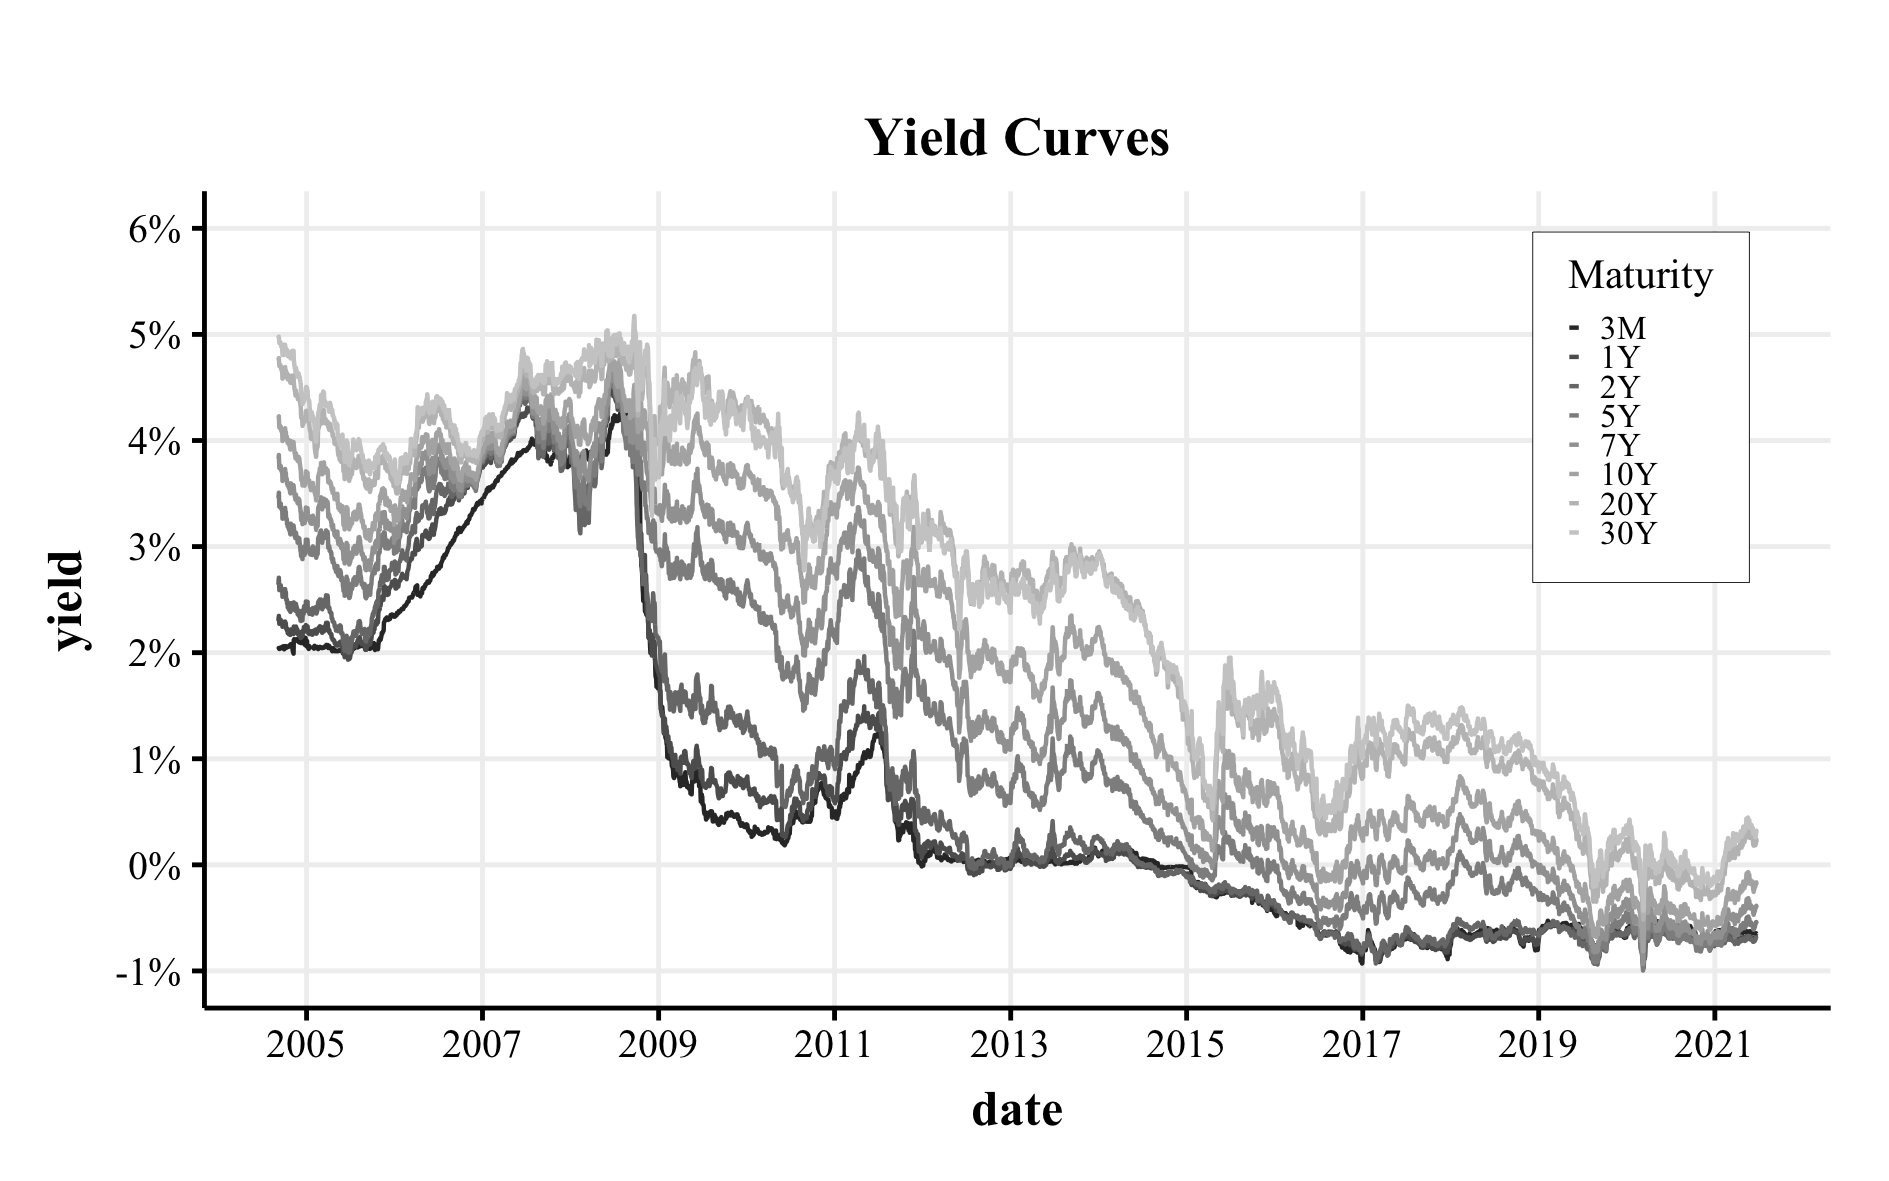
\includegraphics[width=0.7\textwidth]{Figures/yield_curves.png}
% 	\caption{Eurozone yield curves (spot rates) with maturities of 3 months, 1-, 2-, 5-, 7-, 10-, 20-, 30-years; daily frequency; September 2004 - June 2021; consisting of government  nominal bonds whose rating is triple A. (European Central Bank)}
% 	\label{fig:fig1}
% \end{figure}
 
%%%%%%%%%%%%%%%%%%%%%%%%%%%%%%%%%%%%%%%%%%%%%%%%%%%%%%%%%%%%%%%%%%%%%%

\subsection{Control Variables}
To isolate the effect of the speeches, I control for the day-of-the-week effects, the monetary policy shocks, and the surprises of the various macroeconomic news as recommended by the literature (see, e.g., \cite{ehrmann2007,rozkrut2007}). I use the change in the Eonia rate as a measure of monetary policy shocks. I obtain daily data for the Eonia rate from the ECB website covering the period from 2003 to 2021 (see Table \ref{tab:dates}). To control for the macroeconomic surprises, I use the Euro area Citigroup Economic Surprise Index (CESI), which is the weighted moving average of all macroeconomic news surprises relevant to the Euro area. CESI is compiled by Bloomberg and a positive (negative) reading of the CESI suggests that economic news have on balance beaten (fall back) consensus expectations. I gathered CESI from Refinitiv. My Euro area CESI data covers the period from 2003 to 2021 (see Table \ref{tab:dates}).

\section{Methodology}
\subsection{Speech Data Set Preparation}

%%%%%%%%%%%%%%%%%%%%%%%%%%%%%%%%%%%%%%%
\subsection{Measuring the Tone in ECB Speeches}

\subsubsection{The Picault and Renault dictionary}
The measure of the monetary policy sentiment of each speech when using the PR dictionary is expressed as follows:

\begin{equation}
    Tone_{PR_{MP}}=\frac{\#Dovish-\#Hawkish}{\#Dovish+\#Hawkish}
\end{equation}

Similarly, the measure of the economic outlook sentiment:

\begin{equation}
    Tone_{PR_{EC}}=\frac{\#Positive-\#Negative}{\#Positive+\#Negative}
\end{equation}


%%%%%%%%%%%%%%%%%%%%%%%%%%%%%%%%%%%%%%%%%
\subsubsection{The Bennani and Neuenkirch dictionary}

\begin{equation}
    Tone_{BN_{MP}}=\frac{\#Dovish-\#Hawkish}{\#Dovish+\#Hawkish}
\end{equation}

%%%%%%%%%%%%%%%%%%%%%%%%%%%%%%%%%%%%%%%%%

\subsubsection{The Loughran and McDonald dictionary}

The LM dictionary was constructed from the 10-K reports, and it consists of 354 (2355) words that convey a positive (negative) tone in financial and economic contexts. I used \textit{pysentiment2} package available in python to apply the LM dictionary on the ECB's raw speeches. This package is specifically designed for the LM dictionary, and it has an integrated tokenization function. Therefore, no manual text preparation was required. The specific code used can be viewed under the \textit{pysentiment2} documentation \footnote{\href{https://nickderobertis.github.io/pysentiment/}{See \textit{pysentiment2} documentation here}}. Table \ref{tab:LMpython} shows the output returned. The first six columns are speech data set that I provided to the Python. Column seven and eight shows the count of positive and negative words within a particular speech. For example, on May 27th 2021, Isabel Schnabel's speech is counted to have 67 positive and 111 negative words. In the last column \textit{pysentiment2} package even calculates the tone of each speech and it does so according to the following formula:

\begin{equation}
    Tone_{LM}=\frac{\#Positive-\#Negative}{\#Positive+\#Negative}
\end{equation}

This is the same tone measure that I selected for the PR and BN dictionaries. Therefore, the interpretation of the tone score in Table \ref{tab:LMpython} is analogous to the interpretation of the tone scores under the PR and BN dictionaries. The LM tone scores are  used to test my hypotheses. 


\begin{table} [!ht]
\caption{LM Dictionary Python Output}
\label{tab:LMpython}
\begin{adjustbox}{width=\textwidth}
\centering
\begin{tabular}{llp{0.27\linewidth}p{0.27\linewidth}p{0.27\linewidth}lrrr}
\toprule
Date & Speakers & Title & Subtitle & Contents & Role & Positive & Negative & Tone\\
\midrule
2021-05-27 & Isabel Schnabel & Societal responsibility and central bank independence & Keynote speech by Isabel Schnabel, … & SPEECH  Societal responsibility and central  … & Board Members & 67 & 111 & -0.25\\
2021-05-27 & Luis de Guindos & Climate change and financial integration & Keynote speech by Luis de … & SPEECH  Climate change and financial … & Vice-President & 67 & 73 & -0.04\\
2021-05-19 & Fabio Panetta & At the edge of tomorrow: preparing the future of European retail payments & Introductory remarks by Fabio Panetta, … & SPEECH  At the edge of  … & Board Members & 16 & 7 & 0.39\\
2021-05-06 & Christine Lagarde & Towards a green capital markets union for Europe & Speech by Christine Lagarde, President … & SPEECH  Towards a green capital … & President & 50 & 25 & 0.33\\
2021-04-29 & Frank Elderson & All the way to zero: guiding banks towards a carbon-neutral Europe & Keynote speech by Frank Elderson, … & SPEECH  All the way to  … & Board Members & 52 & 64 & -0.10\\
2021-04-26 & Philip R. Lane & Maximising the user value of statistics: lessons from globalisation and the pandemic & Speech by Philip R. Lane, … & SPEECH  Maximising the user value … & Board Members & 70 & 64 & 0.04\\
2021-04-26 & Fabio Panetta & Monetary autonomy in a globalised world & Welcome address by Fabio Panetta, … & SPEECH  Monetary autonomy in a  … & Board Members & 50 & 105 & -0.35\\
2021-04-14 & Fabio Panetta & A digital euro to meet the expectations of Europeans & Introductory remarks by Fabio Panetta, … & SPEECH  A digital euro to … & Board Members & 42 & 39 & 0.04\\
2021-04-14 & Luis de Guindos & Presentation of the ECB Annual Report 2020 … & Introductory remarks by Luis de … & SPEECH  Presentation of the ECB … & Vice-President & 21 & 50 & -0.41\\
2021-04-08 & Christine Lagarde & IMFC Statement & Statement by Christine Lagarde, President … & SPEECH  IMFC Statement Statement by … & President & 32 & 58 & -0.29\\
\dots & \dots & \dots & \dots & \dots & \dots & \dots & \dots & \dots\\
\bottomrule
\end{tabular}
\end{adjustbox}
\end{table}


%%%%%%%%%%%%%%%%%%%%%%%%%%%%%%%%%%%%%%%%%
\subsection{The Econometric Model}


\subsubsection{Baseline Model}



%\begin{equation}
%    ln(h_{t})=\omega + \theta_{1} (|\frac{\varepsilon_{t-1}}{\sqrt{h_{t-1}}}|-\sqrt \frac{2}{\pi}) + \theta_{2} (\frac{\varepsilon_{t-1}}{\sqrt{h_{t-1}}}) + \theta_{3} ln(h_{t-1}) + \kappa^{MP}SD^{MP}_{t} + \kappa^{EC}SD^{EC}_{t} + \phi XD_{t}
%\end{equation}

\subsubsection{Extended Model for Speaker Rank}
I modify my model to determine whether the yield curves are affected differently to speeches by different groups of policy makers within the Executive Board of ECB. I extract three roles - president, vice-president and the remaining policy makers which I simply denominate as board members. 


President vs Vice-president


President vs Board members 


Vice-president vs Board members 




\section{Descriptive Statistics}

\subsection{First Look into Raw Speeches}

\begin{figure}[H]
    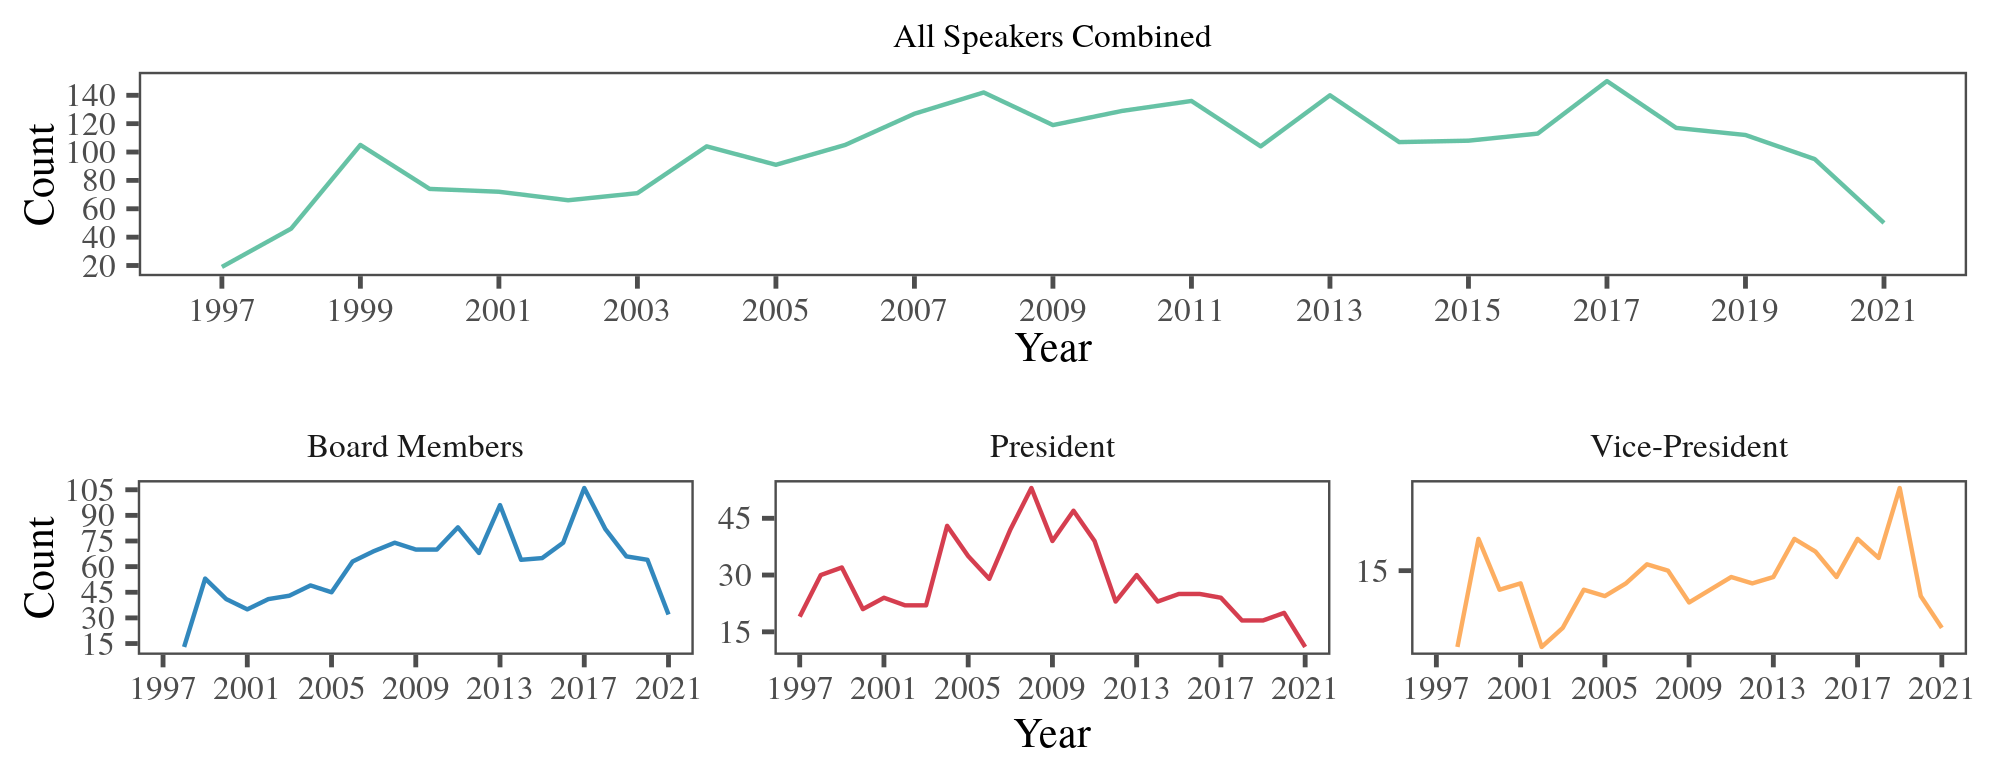
\includegraphics[width = \textwidth]{figures/figcombo3.png}
    \vspace{-9mm}
    \caption{Total Number of Speeches over the Years}
    \label{fig:figcombo3}  
\end{figure}

\begin{figure}[H]
    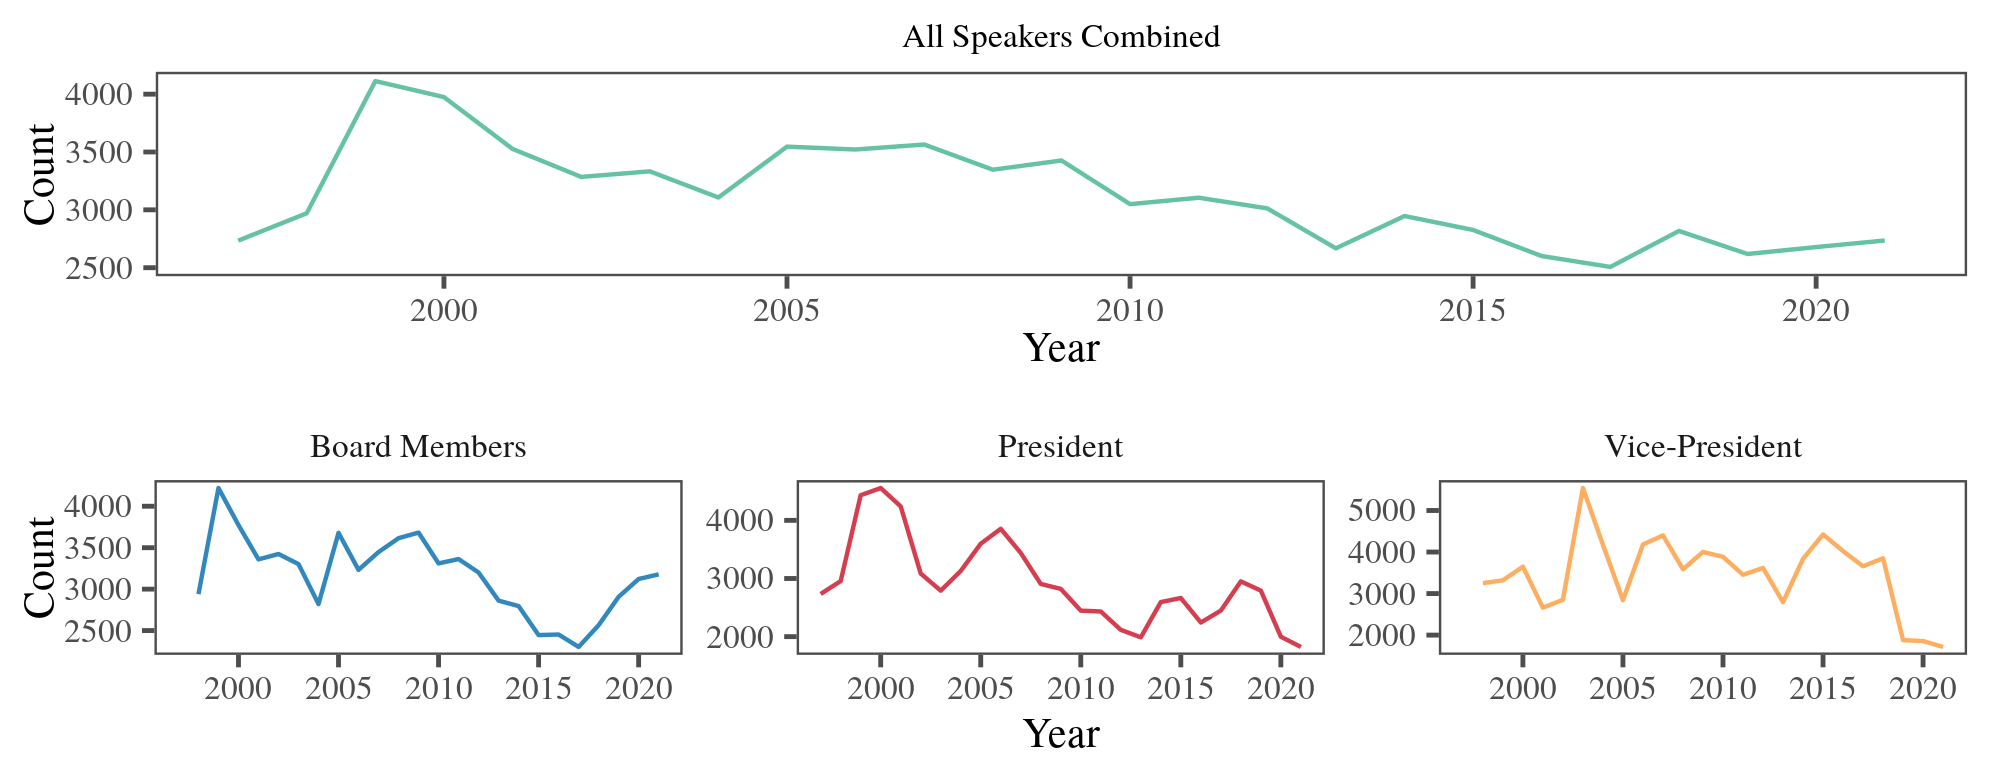
\includegraphics[width = \textwidth]{figures/figcombo1.png}
    \vspace{-9mm}
    \caption{Average Number of Words in a Speech over the Years}
    \label{fig:figcombo1}  
\end{figure}

\begin{figure}[H]
    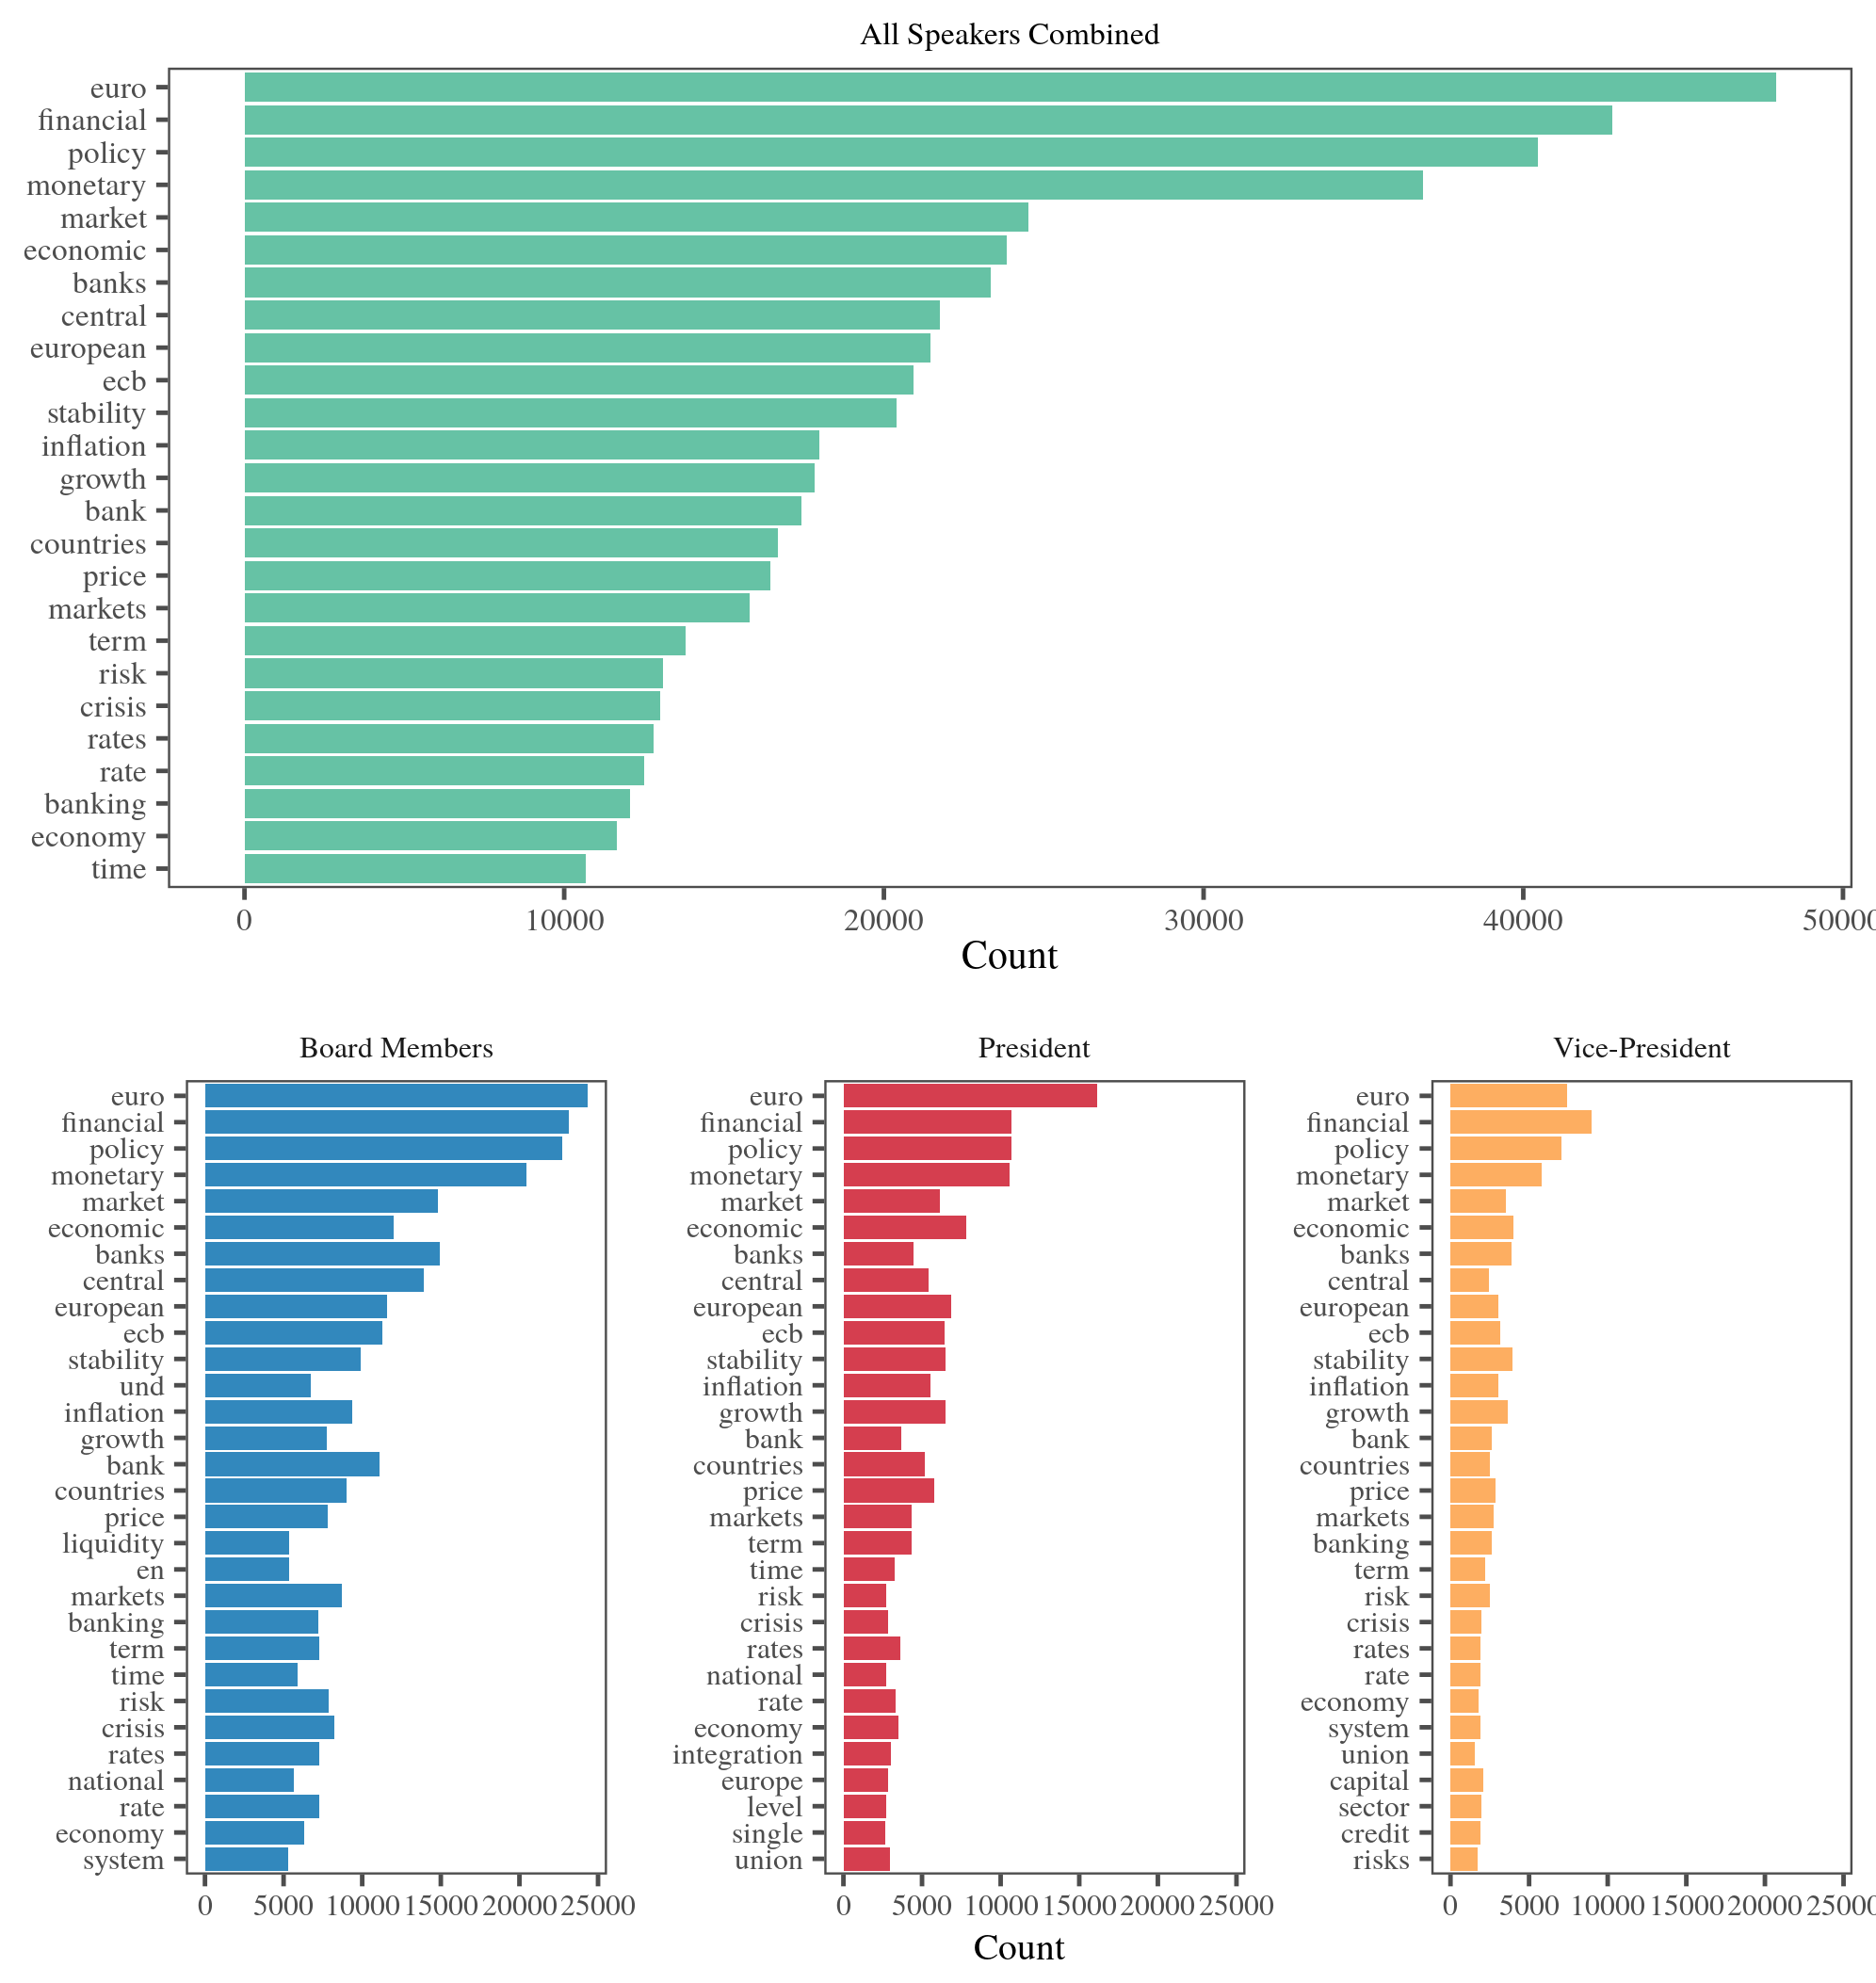
\includegraphics[width = \textwidth]{figures/figcombo2.png}
    \vspace{-9mm}
    \caption{Most Common Words in the Speech Data Set}
    \label{fig:figcombo2}  
\end{figure}

\subsection{Dictionary Sentiments}
\begin{figure}[H]
    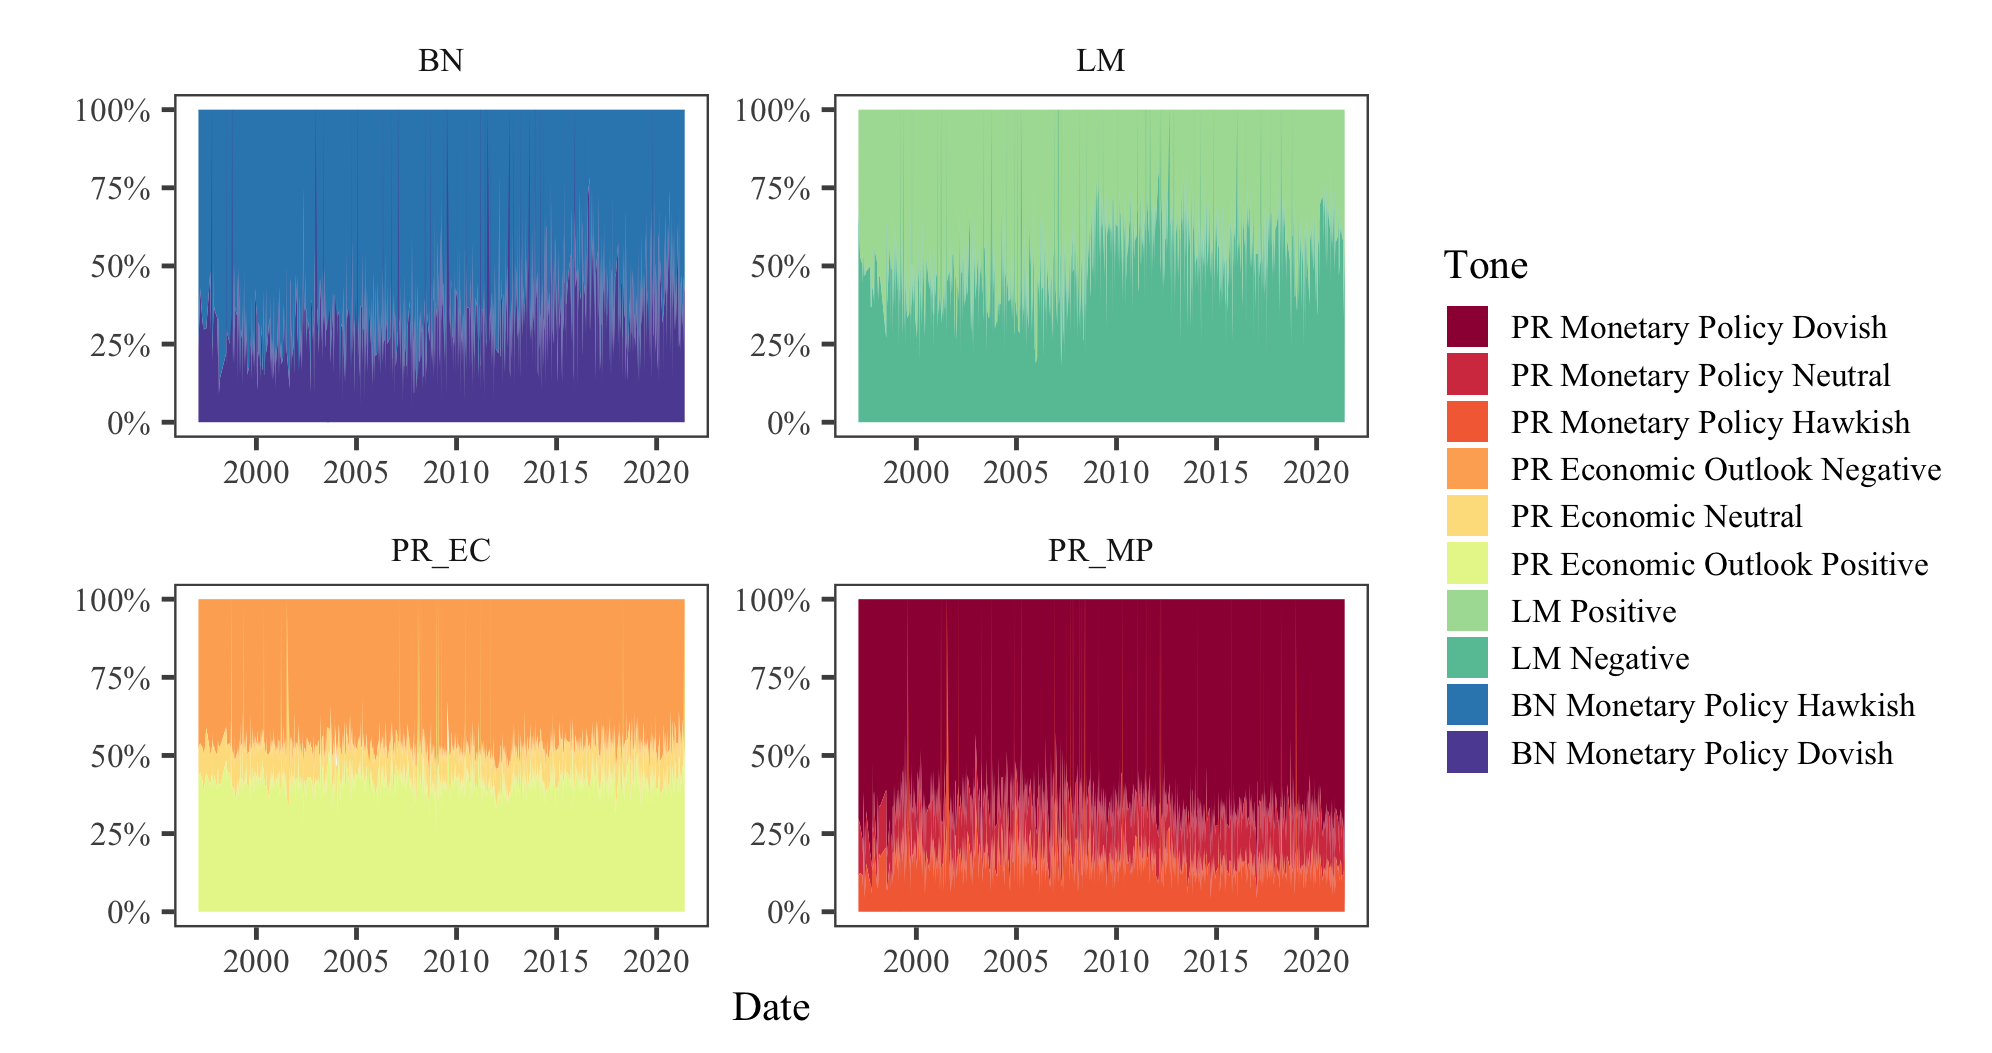
\includegraphics[width = \textwidth]{figures/sentiments.png}
    \vspace{-9mm}
    \caption{Speeches Sentiment Probabilities under PR, BN \& LM Dictionaries}
    \label{fig:sentprob}  
\end{figure}


\begin{figure}[H]
    \centering
    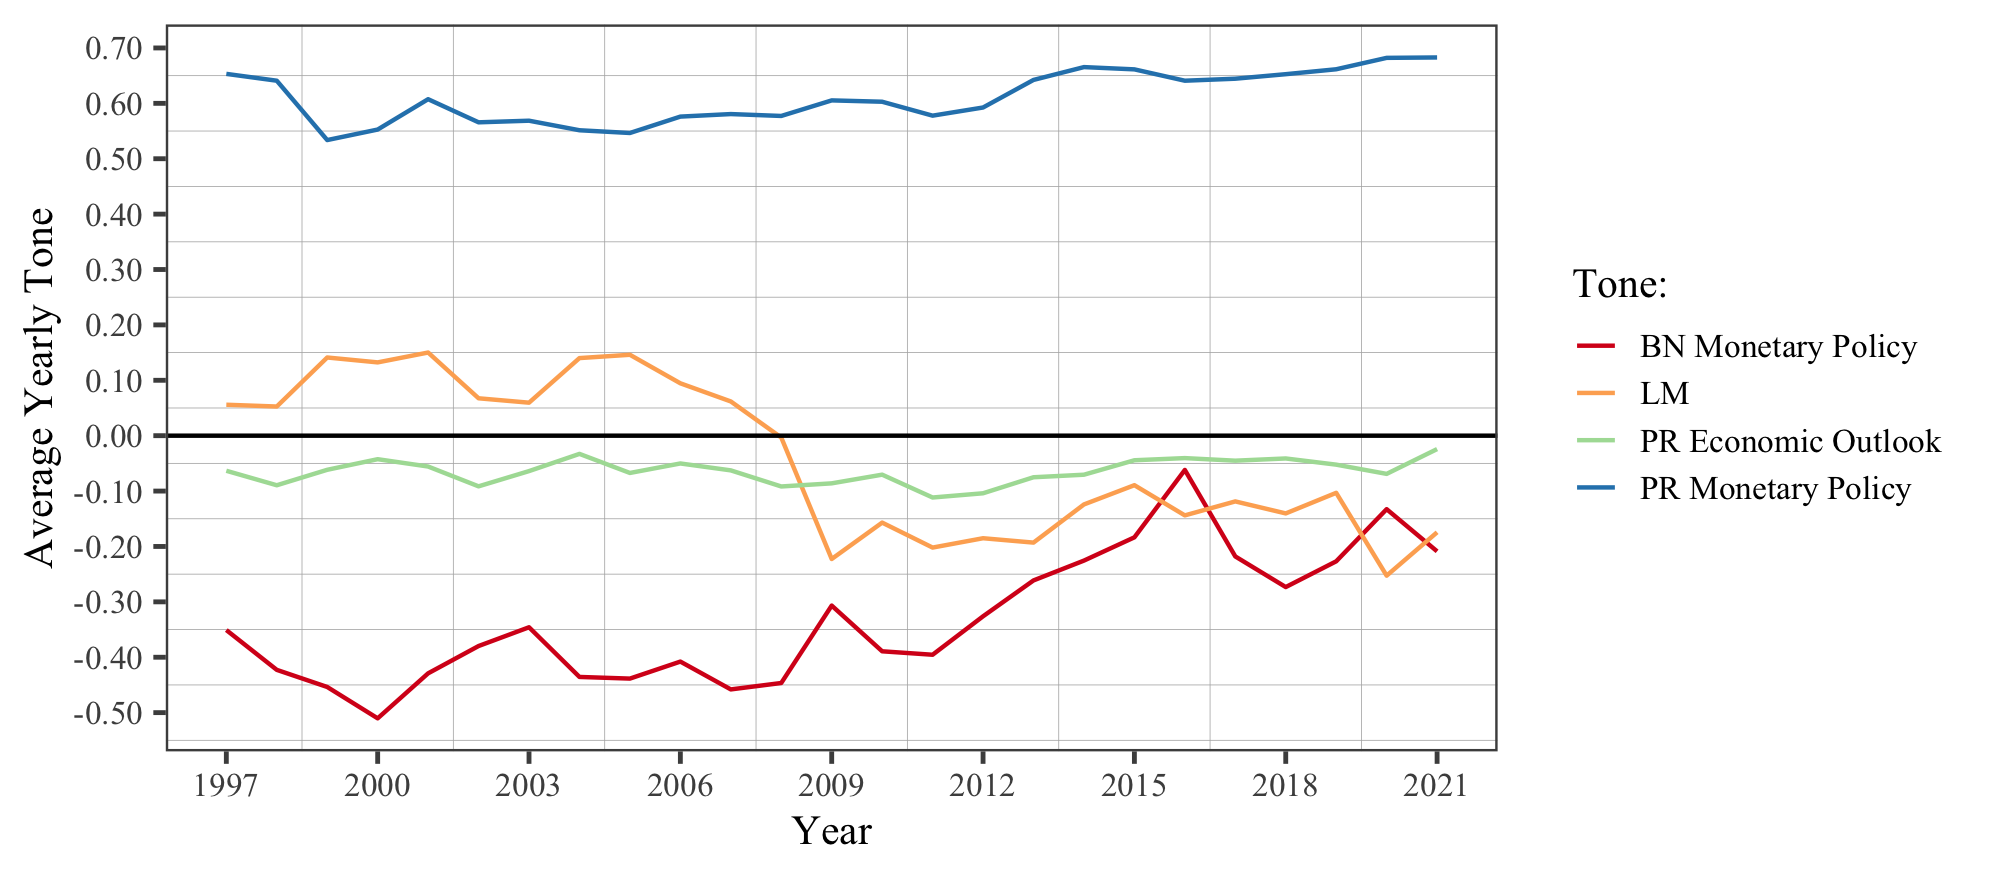
\includegraphics[width =\textwidth]{figures/tones.png}
    \vspace{-3mm}
    \caption{Average Tone of Speeches per Year under PR, BN \& LM Dictionaries}
    \label{fig:avgtones} 
\end{figure}

\subsection{Dictionary Sentiments vs. Asset Prices}

\begin{figure}[H]
    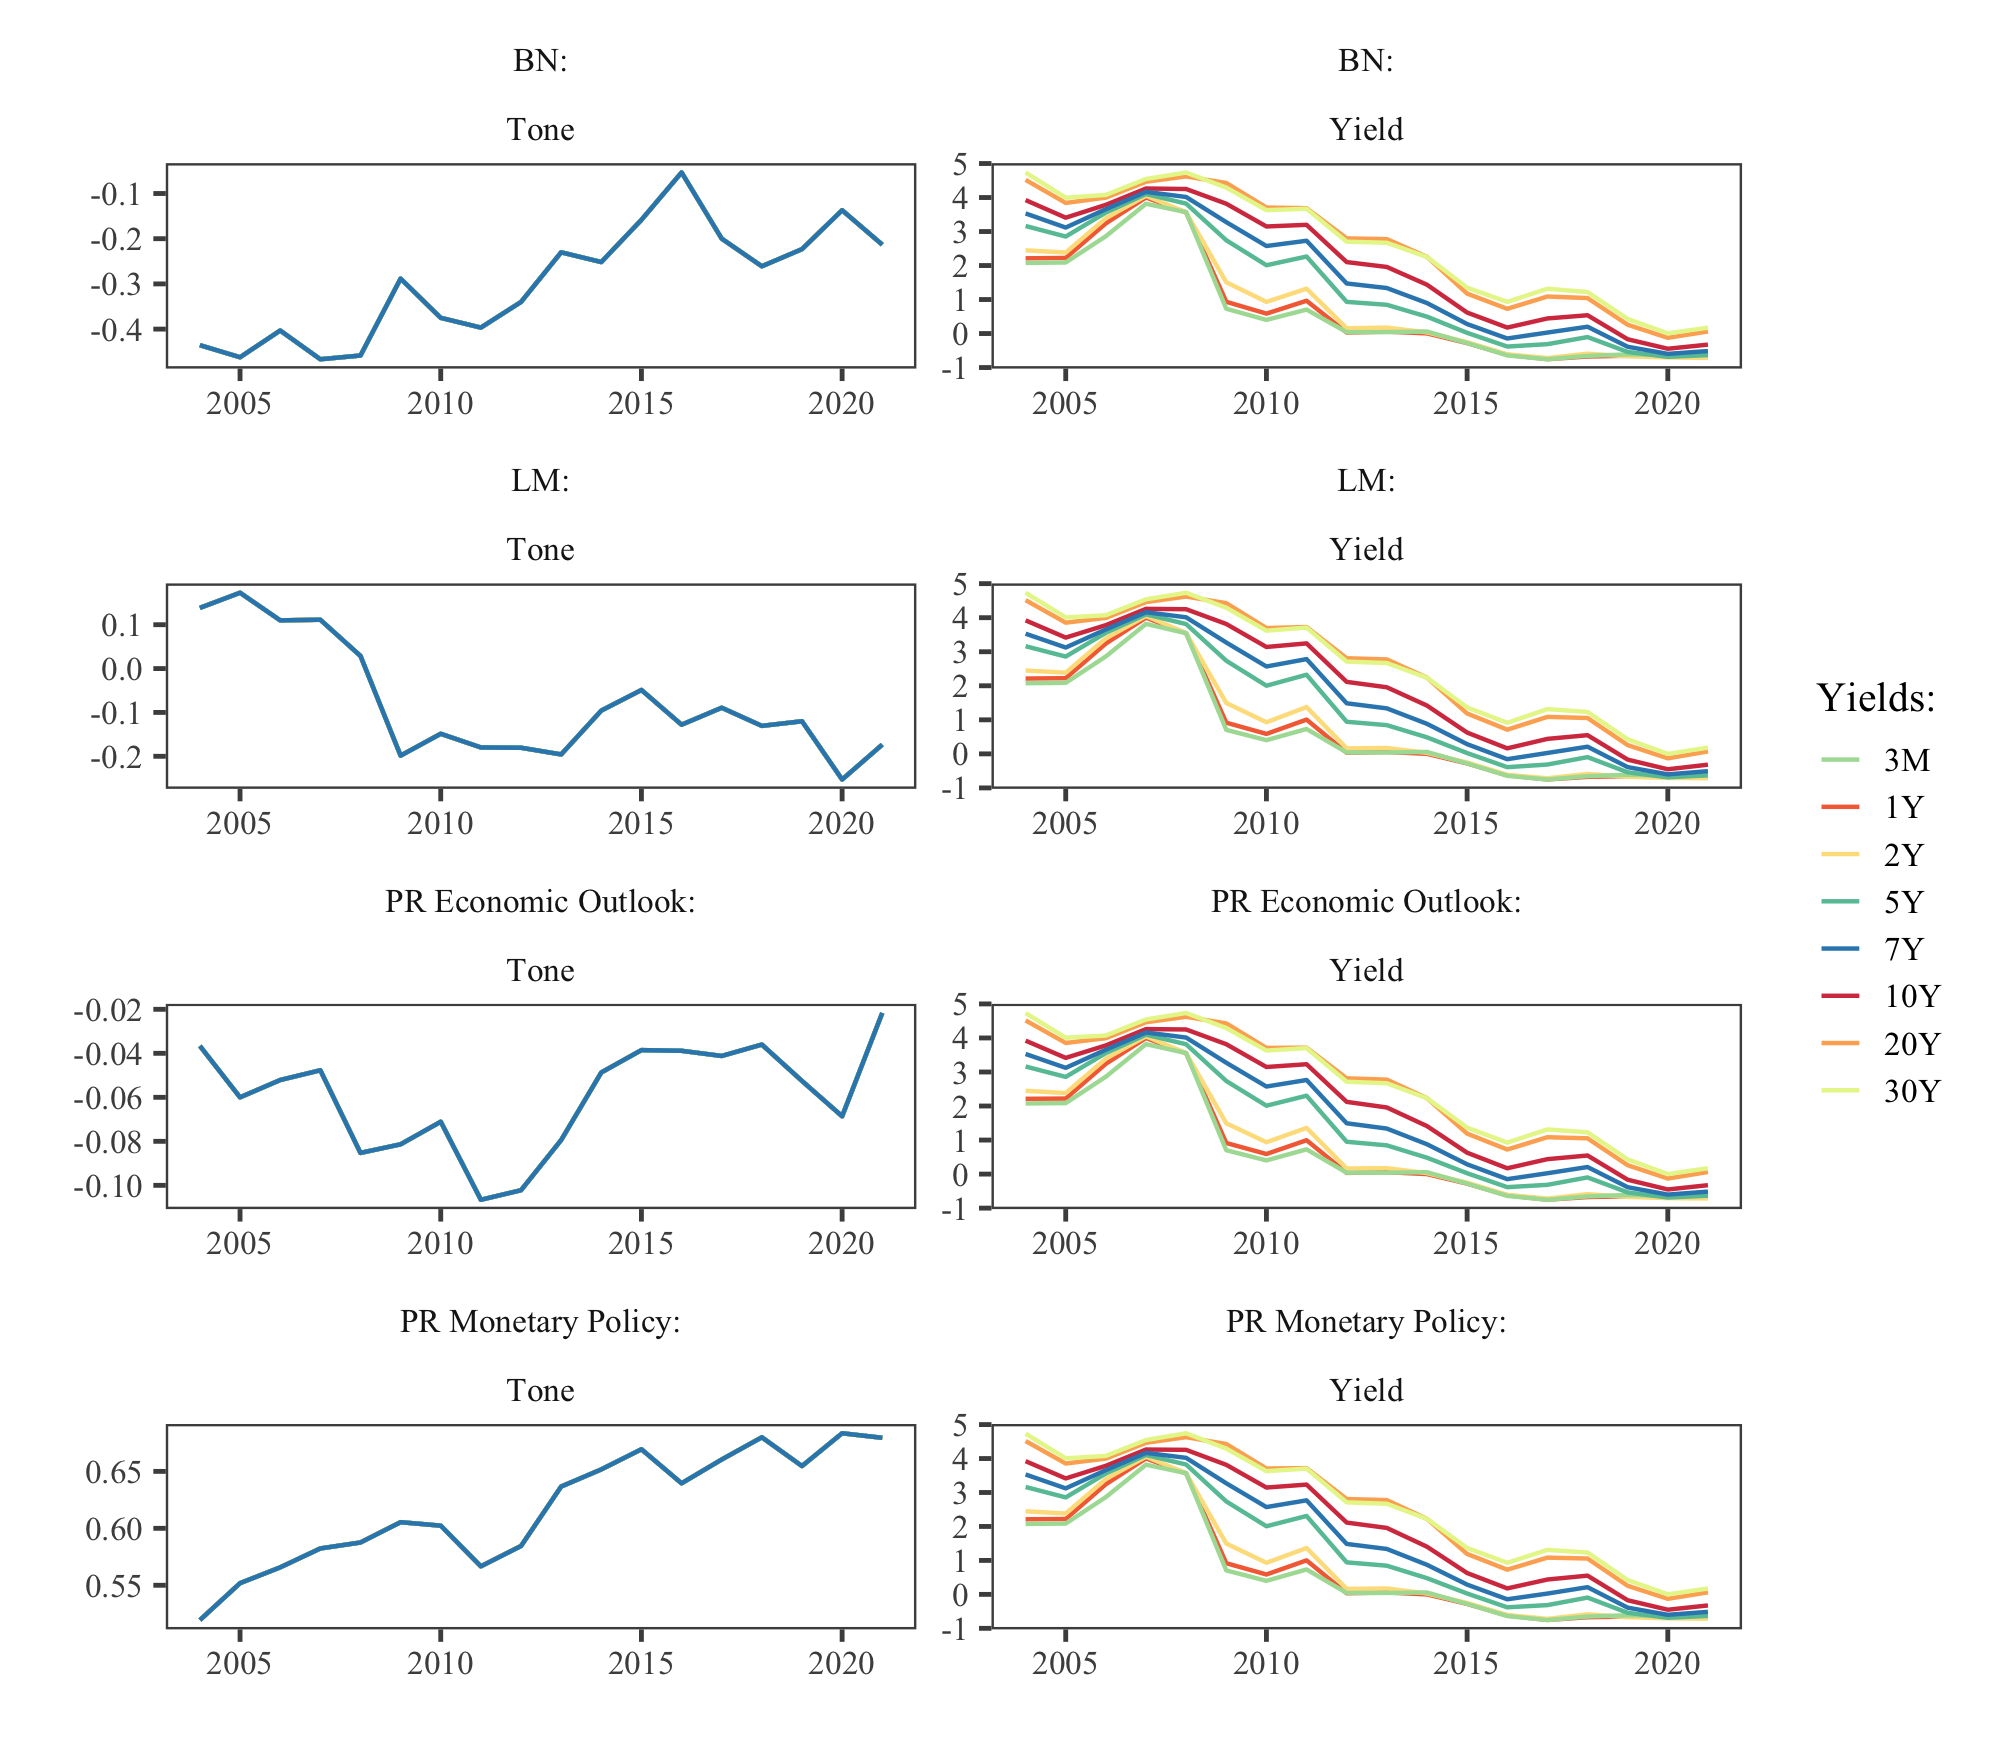
\includegraphics[width = \textwidth]{figures/tonesyields.png}
    \vspace{-9mm}
    \caption{Speeches Sentiment vs Yields under PR, BN \& LM Dictionaries}
    \label{fig:sentyields}  
\end{figure}


\begin{figure}[H]
    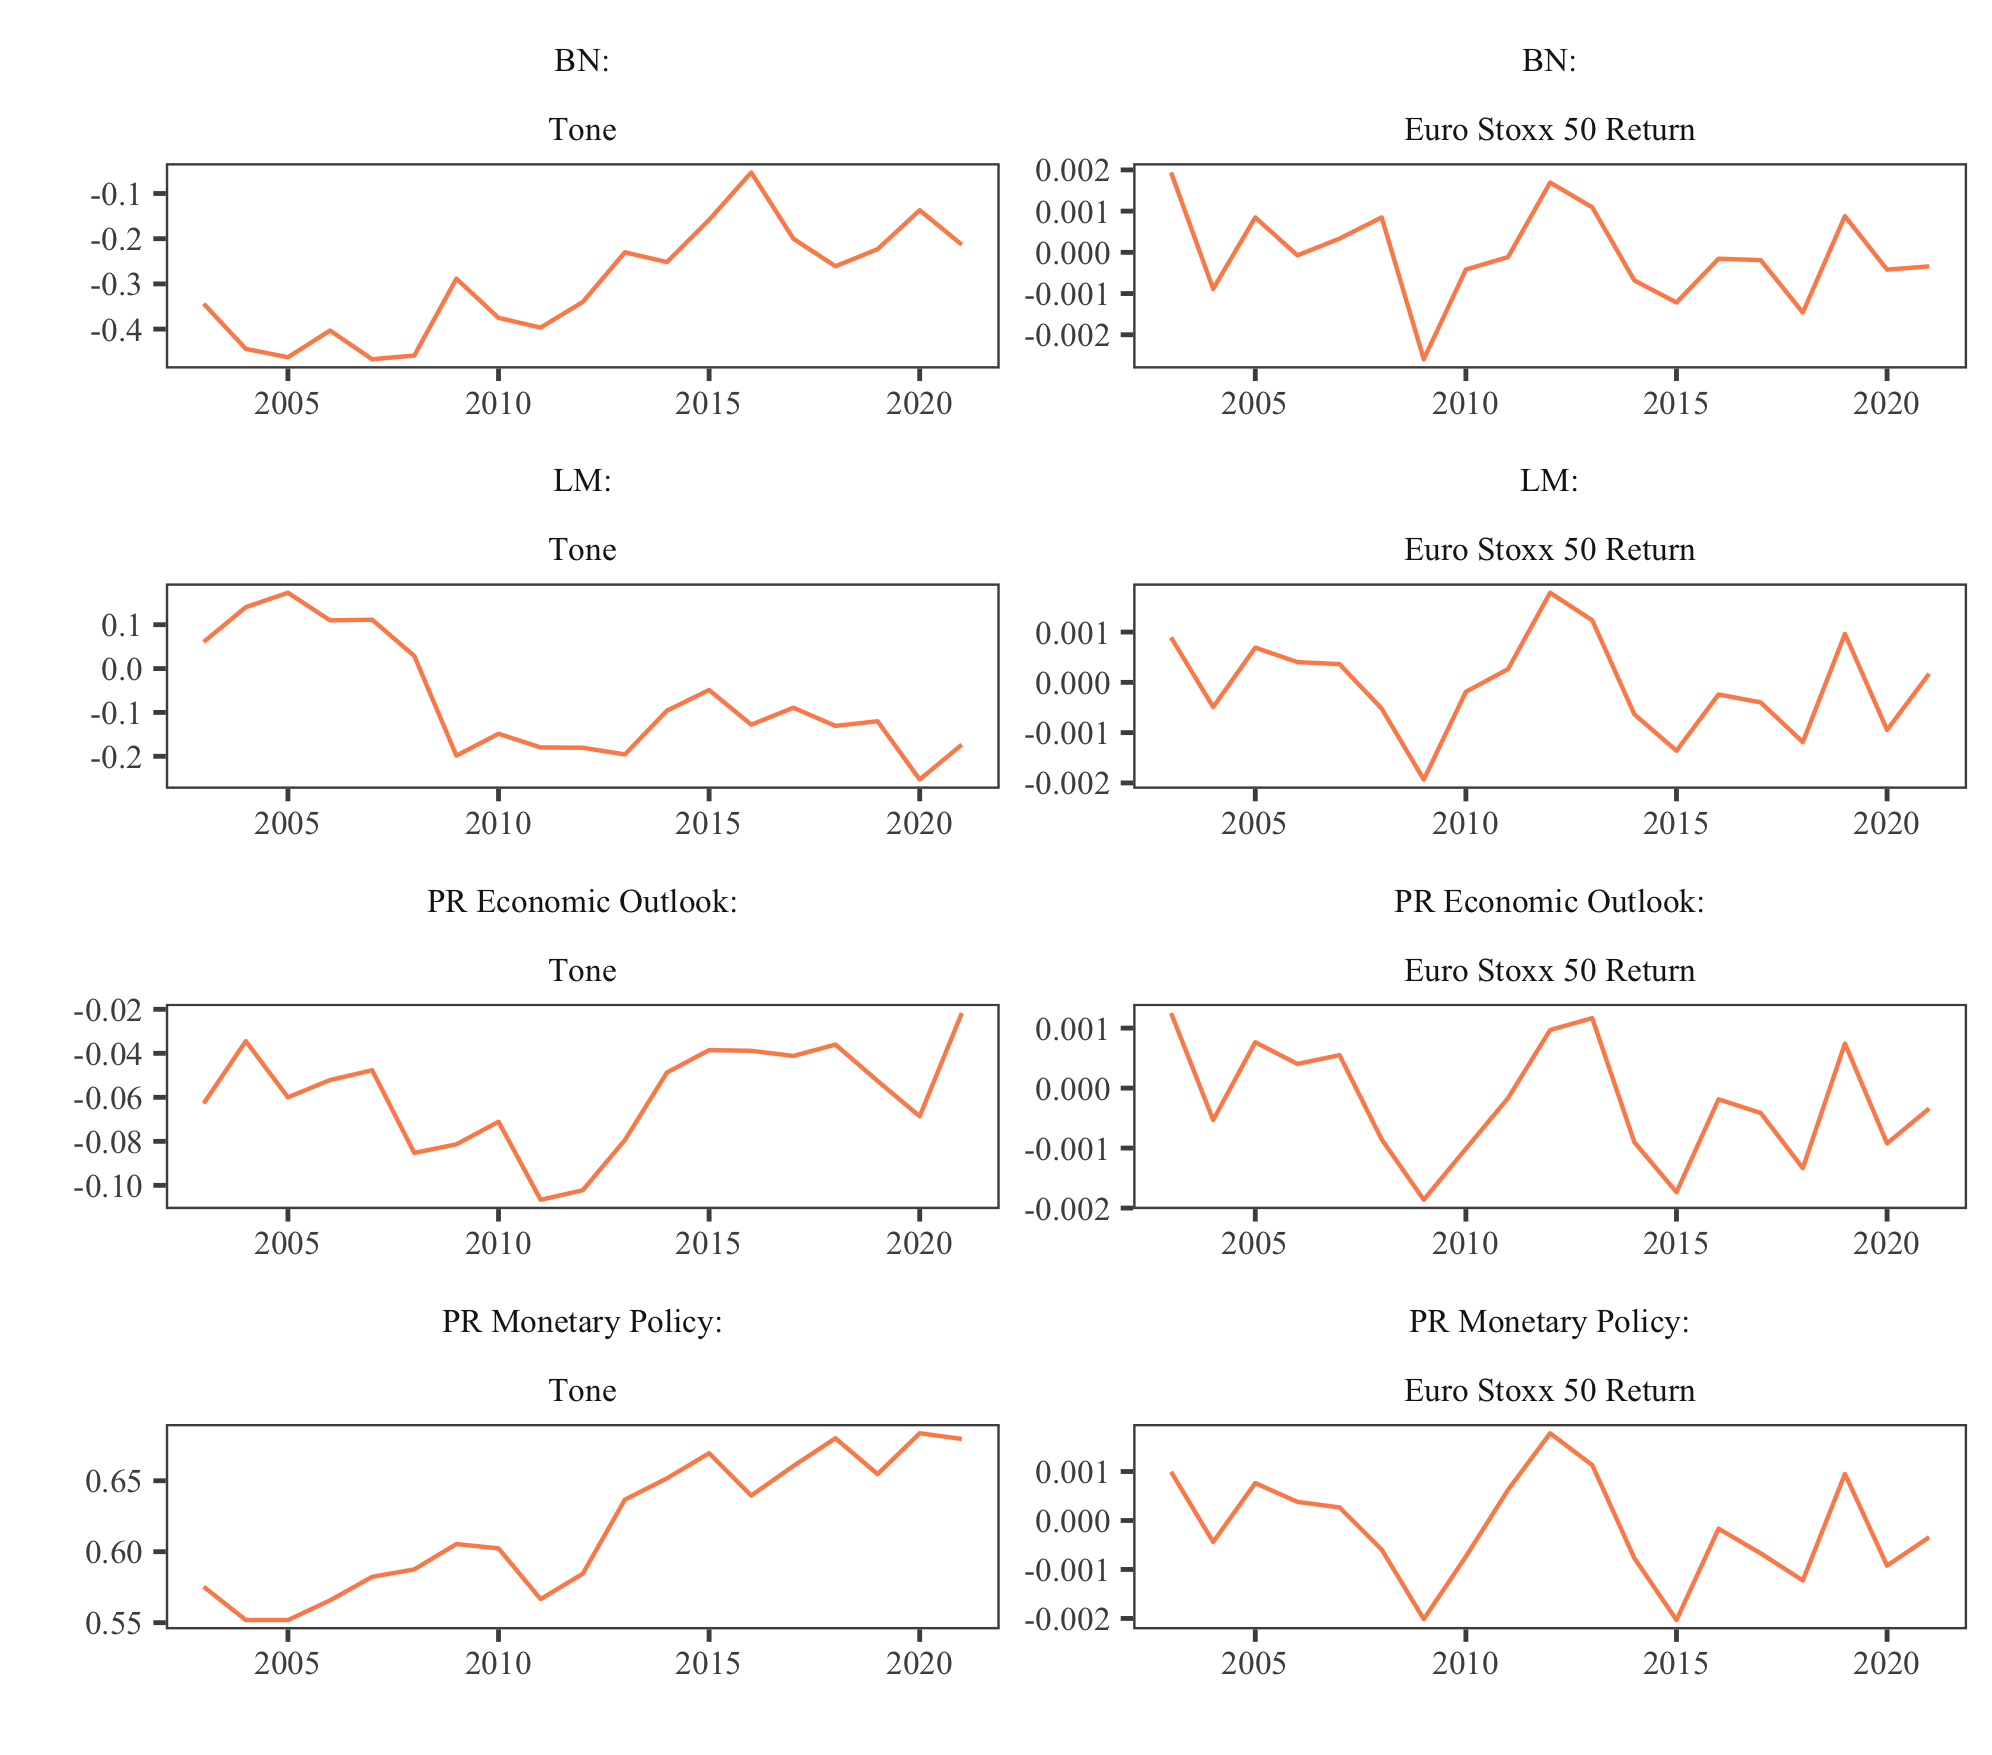
\includegraphics[width = \textwidth]{figures/toneseurostoxx.png}
    \vspace{-9mm}
    \caption{Speeches Sentiment vs. Stock Returns under PR, BN \& LM Dictionaries}
    \label{fig:sentstocks}  
\end{figure}

\begin{figure}[H]
    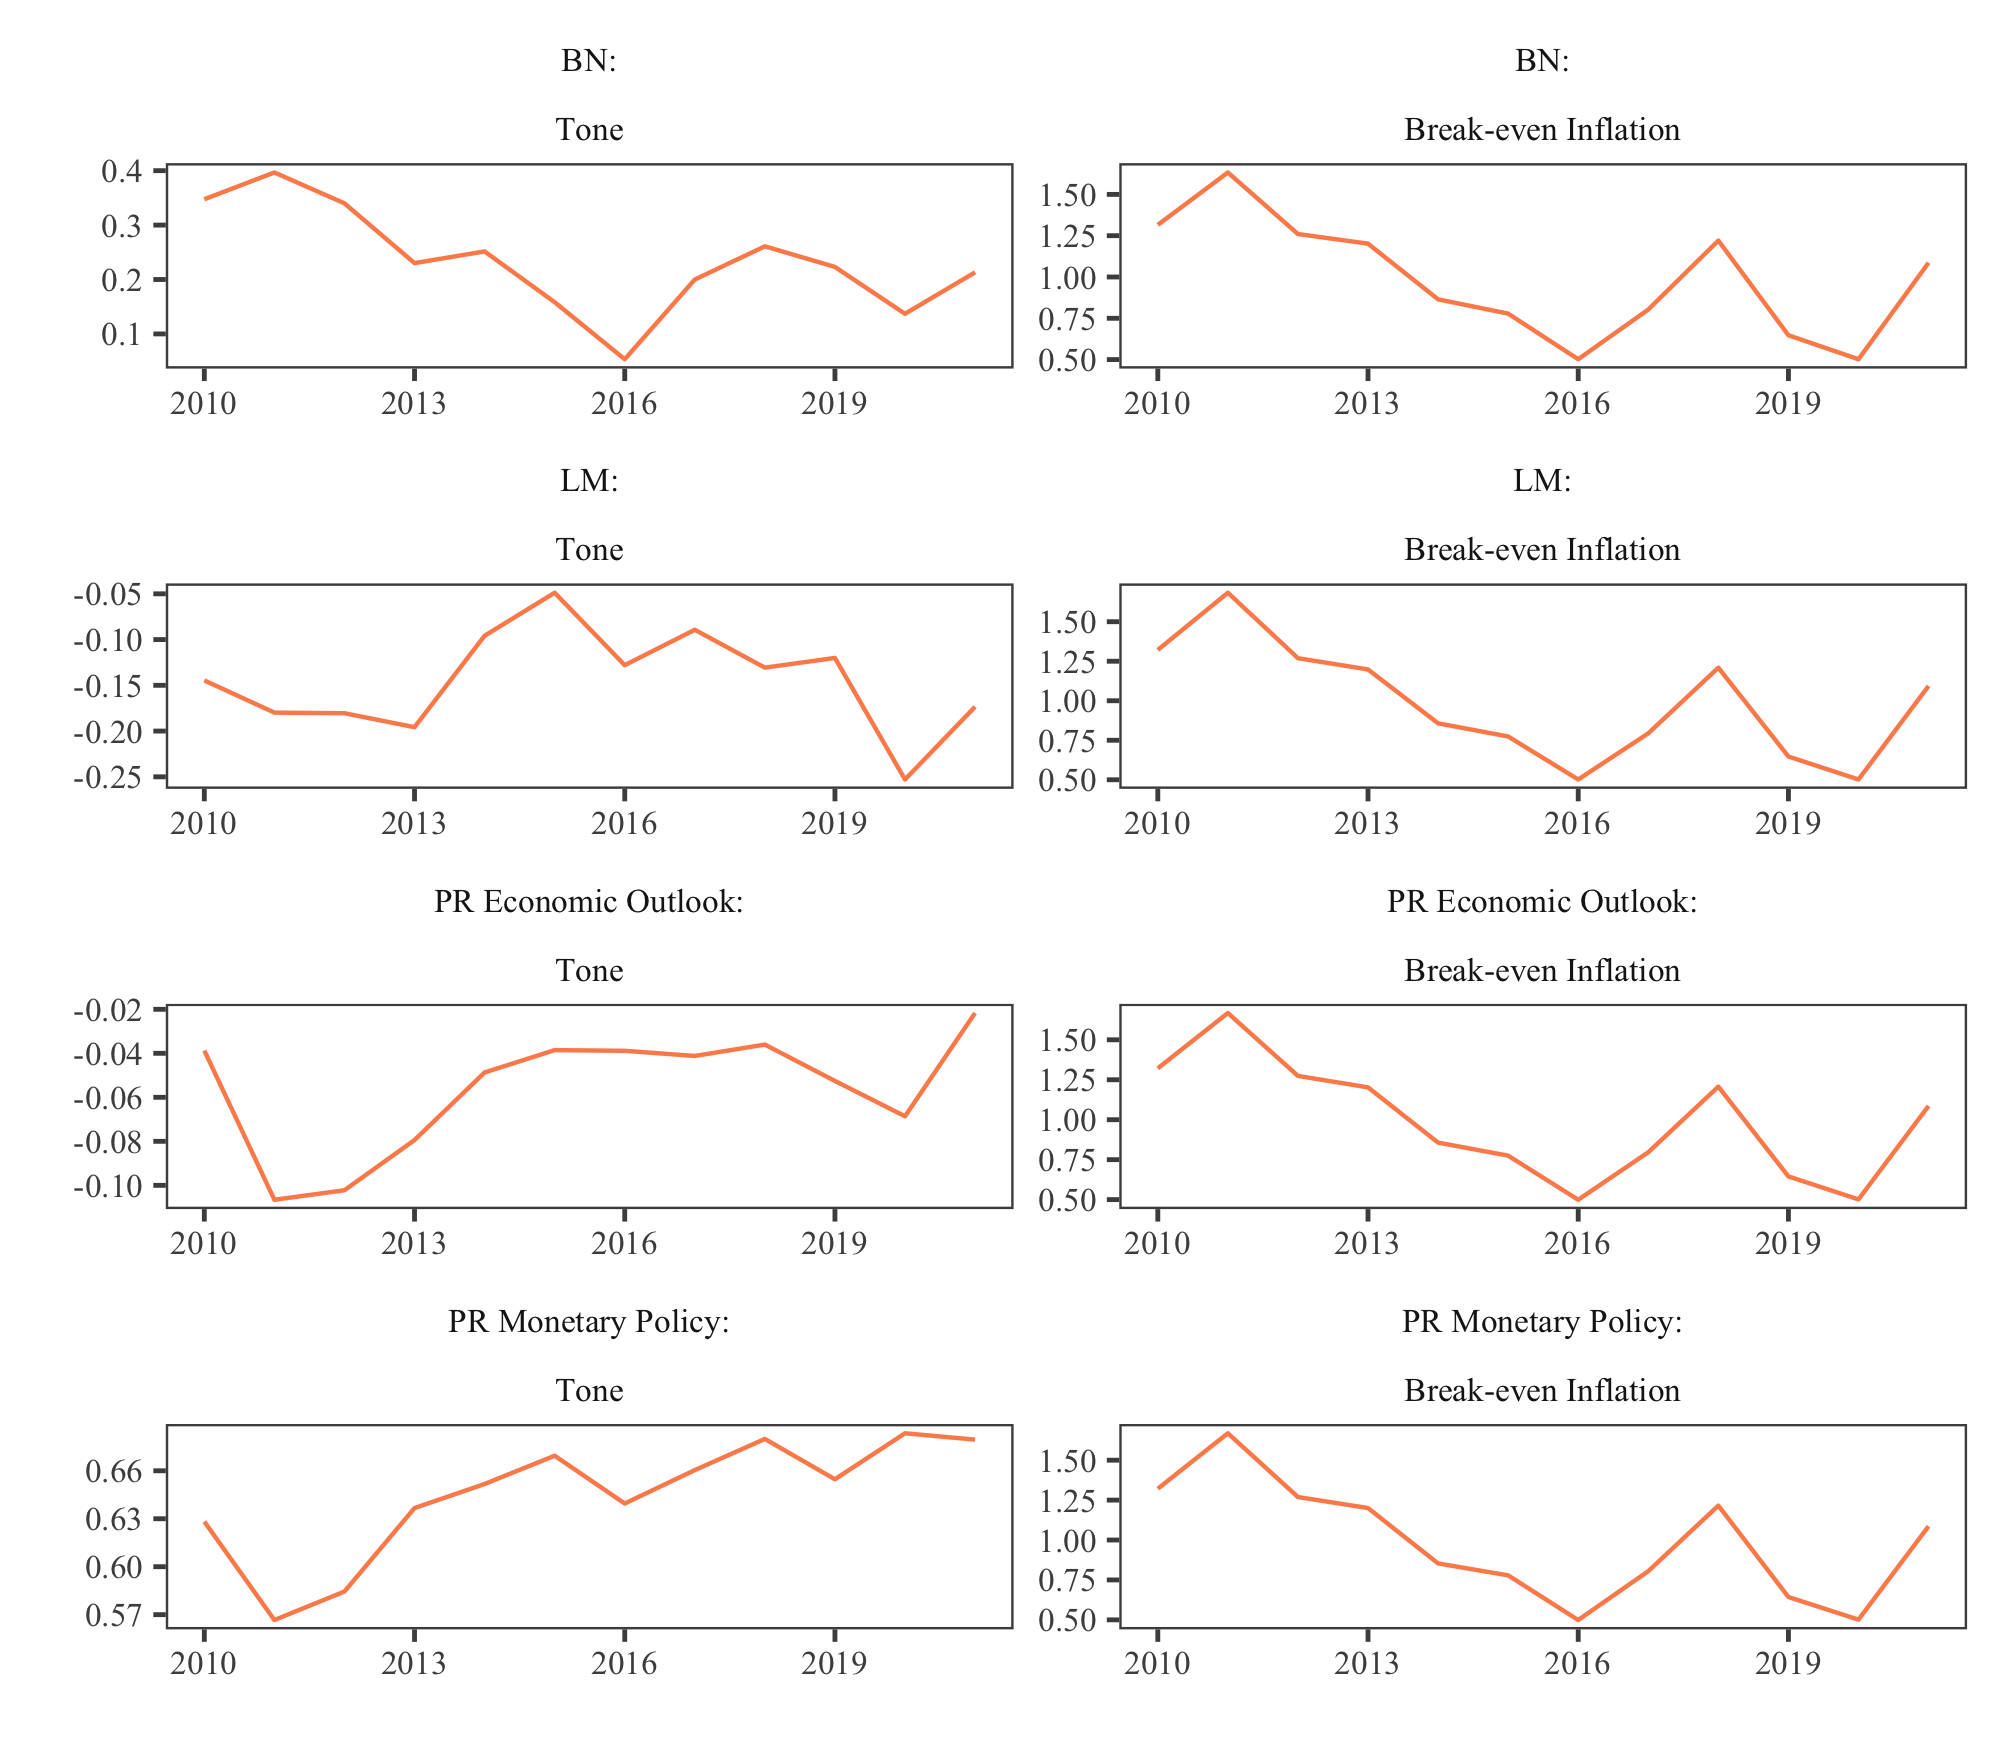
\includegraphics[width = \textwidth]{figures/tonesinflation.png}
    \vspace{-9mm}
    \caption{Speeches Sentiment vs. Inflation Expectation under PR, BN \& LM Dictionaries}
    \label{fig:sentinflation}  
\end{figure}

\begin{figure}[H]
    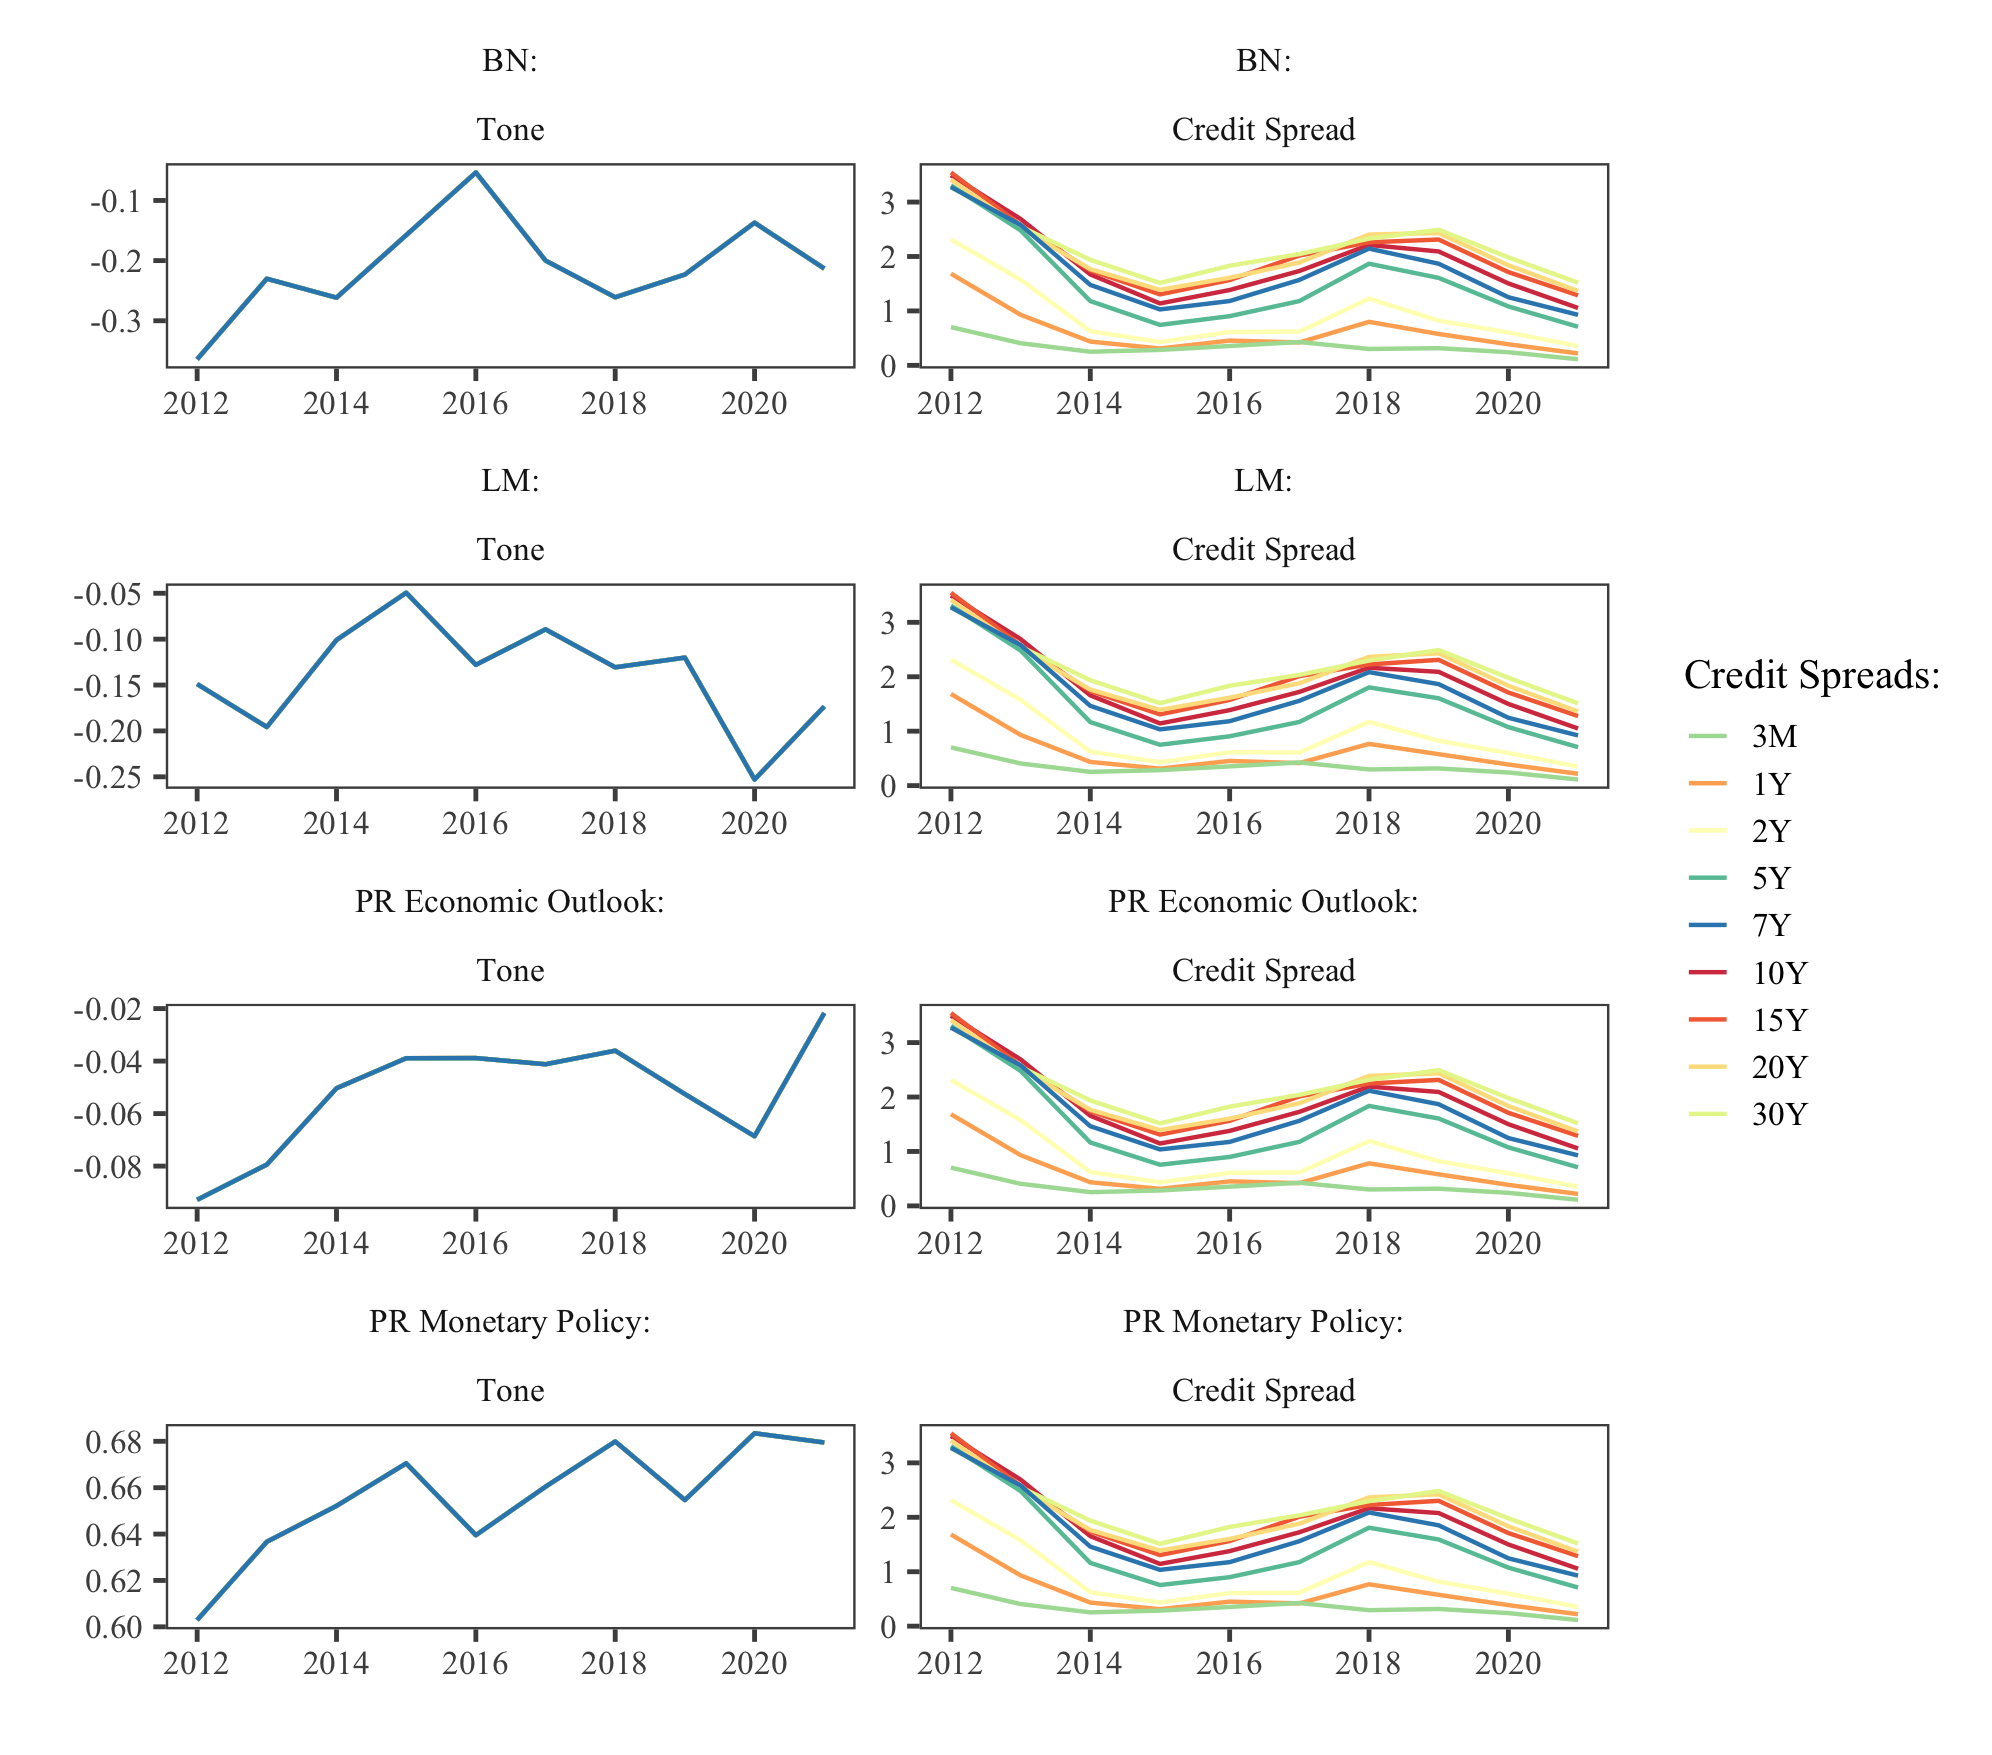
\includegraphics[width = \textwidth]{figures/tonesspreads.png}
    \vspace{-9mm}
    \caption{Speeches Sentiment vs. Credit Spread under PR, BN \& LM Dictionaries}
    \label{fig:senticredit}  
\end{figure}


\subsection{Speaker Sentiment}

\begin{table} [!ht]
\centering
\caption{Speakers' Sentiment proportions under PR, BN \& LM Dictionaries}
\label{speakersent}
\begin{adjustbox}{width=\textwidth}
\begin{tabular}[t]{lrrrrrrrrrr}
\toprule
\multicolumn{1}{c}{ } & \multicolumn{2}{c}{BN} & \multicolumn{2}{c}{LM} & \multicolumn{3}{c}{PR Economic Outlook} & \multicolumn{3}{c}{PR Monetary Policy} \\
\cmidrule(l{3pt}r{3pt}){2-3} \cmidrule(l{3pt}r{3pt}){4-5} \cmidrule(l{3pt}r{3pt}){6-8} \cmidrule(l{3pt}r{3pt}){9-11}
Speaker Rank & Dovish & Hawkish & Positive & Negative & Positive & Neutral & Negative & Dovish & Neutral & Hawkish\\
\midrule
Board Members & 0.388 & 0.612 & 0.423 & 0.577 & 0.413 & 0.106 & 0.481 & 0.699 & 0.156 & 0.145\\
President & 0.338 & 0.662 & 0.497 & 0.503 & 0.421 & 0.101 & 0.477 & 0.665 & 0.160 & 0.176\\
Vice-President & 0.337 & 0.663 & 0.491 & 0.509 & 0.411 & 0.101 & 0.488 & 0.639 & 0.163 & 0.199\\
\bottomrule
\end{tabular}
\end{adjustbox}
\end{table}

%Please see Table \ref{tab:speechtable_descriptives}


\section{Empirical Results}


%\textit{\textbf{Feedback 4:} Include output that answers my questions, hence make subheadings accordingly, the rest of the output place in appendix}

\subsection{Interest Rate Reaction to Speeches}

\subsection{Inflation Expectation Reaction to Speeches}

\subsection{Stock Returns Reaction to Speeches}

\begin{landscape}
    
% Table created by stargazer v.5.2.2 by Marek Hlavac, Harvard University. E-mail: hlavac at fas.harvard.edu
% Date and time: Sat, Aug 14, 2021 - 12:41:33
\begin{table}[!htbp] \centering 
  \caption[PR Monetary Policy Tone \& Interest Rates, Stock Returns, Inflation Expectations: all speeches]{Interest rates, stock returns and inflation expectations reaction to the \textbf{monetary policy} tone embedded in the ECB's speeches under the \textbf{PR dictionary}} 
  \label{tab:assets_all_pr_mp} 
  \begin{adjustbox}{width=1.25\textwidth}
\begin{tabular}{@{\extracolsep{5pt}}lcccccccccc} 
\\[-1.8ex]\hline 
\hline \\[-1.8ex] 
 & \multicolumn{10}{c}{\textit{Dependent variable:}} \\ 
\cline{2-11} 
\\[-1.8ex] & \multicolumn{10}{c}{Interest rates, stock returns and inflation expectations} \\ 
 & 3M & 1Y & 2Y & 5Y & 7Y & 10Y & 20Y & 30Y & Eurostoxx & Breakeven-inflation \\ 
\\[-1.8ex] & (1) & (2) & (3) & (4) & (5) & (6) & (7) & (8) & (9) & (10)\\ 
\hline \\[-1.8ex] 
 polarity & $-$0.002 & 0.003 & 0.007 & 0.011$^{*}$ & 0.010$^{*}$ & 0.009 & 0.009 & 0.013$^{*}$ & 0.003 & 0.001 \\ 
  & (0.004) & (0.004) & (0.006) & (0.006) & (0.006) & (0.006) & (0.007) & (0.007) & (0.002) & (0.008) \\ 
  & & & & & & & & & & \\ 
 dependent\_l1 & $-$0.010 & 0.199$^{***}$ & 0.130$^{***}$ & 0.109$^{***}$ & 0.115$^{***}$ & 0.122$^{***}$ & 0.138$^{***}$ & 0.122$^{***}$ & $-$0.705$^{***}$ & $-$0.073$^{**}$ \\ 
  & (0.021) & (0.029) & (0.029) & (0.028) & (0.028) & (0.028) & (0.027) & (0.026) & (0.024) & (0.037) \\ 
  & & & & & & & & & & \\ 
 dependent\_l2 & 0.110$^{***}$ & $-$0.0005 & 0.015 & 0.032 & 0.026 & 0.013 & $-$0.017 & $-$0.017 & $-$0.321$^{***}$ & 0.006 \\ 
  & (0.031) & (0.028) & (0.029) & (0.028) & (0.028) & (0.028) & (0.027) & (0.024) & (0.025) & (0.023) \\ 
  & & & & & & & & & & \\ 
 eonia & $-$0.018$^{**}$ & 0.021$^{**}$ & 0.020 & 0.009 & $-$0.001 & $-$0.011 & $-$0.012 & 0.002 & 0.011$^{*}$ & 0.033 \\ 
  & (0.008) & (0.009) & (0.013) & (0.014) & (0.014) & (0.014) & (0.015) & (0.016) & (0.005) & (0.027) \\ 
  & & & & & & & & & & \\ 
 eonia\_l1 & 0.007 & 0.004 & 0.010 & $-$0.007 & $-$0.015 & $-$0.021 & $-$0.018 & 0.001 & $-$0.002 & 0.029 \\ 
  & (0.007) & (0.009) & (0.012) & (0.013) & (0.013) & (0.013) & (0.014) & (0.015) & (0.005) & (0.027) \\ 
  & & & & & & & & & & \\ 
 cesi\_eur & 0.0001 & 0.0003$^{***}$ & 0.0004$^{***}$ & 0.001$^{***}$ & 0.001$^{***}$ & 0.001$^{***}$ & 0.001$^{***}$ & 0.001$^{***}$ & 0.00001 & $-$0.00004 \\ 
  & (0.0001) & (0.0001) & (0.0001) & (0.0001) & (0.0001) & (0.0001) & (0.0002) & (0.0002) & (0.0001) & (0.0002) \\ 
  & & & & & & & & & & \\ 
 cesi\_eur\_l1 & $-$0.00001 & $-$0.0002$^{**}$ & $-$0.0004$^{***}$ & $-$0.001$^{***}$ & $-$0.001$^{***}$ & $-$0.001$^{***}$ & $-$0.001$^{***}$ & $-$0.001$^{***}$ & $-$0.00001 & 0.00002 \\ 
  & (0.0001) & (0.0001) & (0.0001) & (0.0001) & (0.0001) & (0.0001) & (0.0002) & (0.0002) & (0.0001) & (0.0002) \\ 
  & & & & & & & & & & \\ 
 financial\_crisis\_dummy & $-$0.004$^{***}$ & 0.0001 & 0.003 & 0.005$^{*}$ & 0.005$^{*}$ & 0.005$^{**}$ & 0.006$^{**}$ & 0.007$^{**}$ & 0.001 &  \\ 
  & (0.002) & (0.002) & (0.003) & (0.003) & (0.003) & (0.003) & (0.003) & (0.003) & (0.001) &  \\ 
  & & & & & & & & & & \\ 
 covid\_crisis\_dummy & $-$0.004 & $-$0.001 & 0.0001 & 0.0003 & 0.001 & 0.001 & 0.003 & 0.002 & $-$0.001 & $-$0.004 \\ 
  & (0.002) & (0.003) & (0.004) & (0.004) & (0.004) & (0.004) & (0.004) & (0.005) & (0.002) & (0.004) \\ 
  & & & & & & & & & & \\ 
 polarity:financial\_crisis\_dummy & $-$0.006 & $-$0.009 & $-$0.006 & $-$0.003 & $-$0.004 & $-$0.006 & $-$0.012 & $-$0.016 & $-$0.005 &  \\ 
  & (0.007) & (0.009) & (0.012) & (0.013) & (0.013) & (0.013) & (0.014) & (0.015) & (0.005) &  \\ 
  & & & & & & & & & & \\ 
 polarity:covid\_crisis\_dummy & $-$0.004 & 0.010 & 0.010 & $-$0.007 & $-$0.011 & $-$0.016 & $-$0.028 & $-$0.037 & $-$0.031$^{**}$ & 0.016 \\ 
  & (0.019) & (0.022) & (0.030) & (0.033) & (0.033) & (0.033) & (0.035) & (0.039) & (0.014) & (0.034) \\ 
  & & & & & & & & & & \\ 
 Constant & $-$0.0001 & $-$0.001 & $-$0.002 & $-$0.003$^{**}$ & $-$0.003$^{***}$ & $-$0.003$^{***}$ & $-$0.004$^{***}$ & $-$0.004$^{**}$ & 0.00002 & 0.001 \\ 
  & (0.001) & (0.001) & (0.001) & (0.001) & (0.001) & (0.001) & (0.001) & (0.001) & (0.0005) & (0.001) \\ 
  & & & & & & & & & & \\ 
\hline \\[-1.8ex] 
Observations & 1,249 & 1,249 & 1,249 & 1,249 & 1,249 & 1,249 & 1,249 & 1,249 & 1,355 & 790 \\ 
R$^{2}$ & 0.052 & 0.062 & 0.031 & 0.032 & 0.037 & 0.040 & 0.049 & 0.048 & 0.407 & 0.019 \\ 
Adjusted R$^{2}$ & 0.040 & 0.050 & 0.019 & 0.020 & 0.025 & 0.028 & 0.038 & 0.037 & 0.400 & 0.002 \\ 
Residual Std. Error & 0.021 & 0.024 & 0.033 & 0.036 & 0.035 & 0.036 & 0.038 & 0.042 & 0.015 & 0.037 \\ 
\hline 
\hline \\[-1.8ex] 
\textit{Note:}  & \multicolumn{10}{r}{$^{*}$p$<$0.1; $^{**}$p$<$0.05; $^{***}$p$<$0.01} \\ 
\end{tabular} 
\end{adjustbox} 
\end{table} 

    \end{landscape} 
\begin{landscape}
    
% Table created by stargazer v.5.2.2 by Marek Hlavac, Harvard University. E-mail: hlavac at fas.harvard.edu
% Date and time: Sat, Aug 14, 2021 - 12:41:15
\begin{table}[!htbp] \centering 
  \caption [PR Economic Outlook Tone \& Interest Rates, Stock Returns, Inflation Expectations: all speeches]{Interest rates, stock returns and inflation expectations reaction to the \textbf{economic outlook} tone embedded in the ECB's speeches under the \textbf{PR dictionary}} 
  \label{tab:assets_all_pr_ec} 
  \begin{adjustbox}{width=1.25\textwidth}
\begin{tabular}{@{\extracolsep{5pt}}lcccccccccc} 
\\[-1.8ex]\hline 
\hline \\[-1.8ex] 
 & \multicolumn{10}{c}{\textit{Dependent variable:}} \\ 
\cline{2-11} 
\\[-1.8ex] & \multicolumn{10}{c}{Interest rates, stock returns and inflation expectations} \\ 
 & 3M & 1Y & 2Y & 5Y & 7Y & 10Y & 20Y & 30Y & Eurostoxx & Breakeven-inflation \\ 
\\[-1.8ex] & (1) & (2) & (3) & (4) & (5) & (6) & (7) & (8) & (9) & (10)\\ 
\hline \\[-1.8ex] 
 polarity & 0.002 & 0.002 & 0.002 & 0.004 & 0.004 & 0.002 & $-$0.001 & $-$0.003 & 0.004 & 0.002 \\ 
  & (0.005) & (0.006) & (0.008) & (0.009) & (0.009) & (0.009) & (0.010) & (0.011) & (0.004) & (0.010) \\ 
  & & & & & & & & & & \\ 
 dependent\_l1 & $-$0.009 & 0.194$^{***}$ & 0.130$^{***}$ & 0.117$^{***}$ & 0.123$^{***}$ & 0.130$^{***}$ & 0.149$^{***}$ & 0.131$^{***}$ & $-$0.691$^{***}$ & $-$0.065$^{*}$ \\ 
  & (0.021) & (0.028) & (0.029) & (0.028) & (0.027) & (0.027) & (0.027) & (0.025) & (0.023) & (0.036) \\ 
  & & & & & & & & & & \\ 
 dependent\_l2 & 0.122$^{***}$ & 0.031 & 0.046 & 0.050$^{*}$ & 0.038 & 0.022 & $-$0.012 & $-$0.012 & $-$0.316$^{***}$ & 0.010 \\ 
  & (0.031) & (0.028) & (0.029) & (0.028) & (0.028) & (0.027) & (0.027) & (0.024) & (0.025) & (0.023) \\ 
  & & & & & & & & & & \\ 
 eonia & $-$0.017$^{**}$ & 0.017$^{*}$ & 0.015 & 0.004 & $-$0.005 & $-$0.015 & $-$0.015 & $-$0.002 & 0.009 & 0.027 \\ 
  & (0.008) & (0.009) & (0.012) & (0.014) & (0.014) & (0.014) & (0.015) & (0.016) & (0.005) & (0.027) \\ 
  & & & & & & & & & & \\ 
 eonia\_l1 & 0.006 & 0.007 & 0.013 & $-$0.005 & $-$0.013 & $-$0.020 & $-$0.017 & 0.001 & $-$0.003 & 0.025 \\ 
  & (0.007) & (0.009) & (0.012) & (0.013) & (0.013) & (0.013) & (0.014) & (0.015) & (0.005) & (0.027) \\ 
  & & & & & & & & & & \\ 
 cesi\_eur & 0.00005 & 0.0002$^{**}$ & 0.0004$^{***}$ & 0.0005$^{***}$ & 0.001$^{***}$ & 0.001$^{***}$ & 0.001$^{***}$ & 0.001$^{***}$ & 0.00001 & $-$0.0001 \\ 
  & (0.0001) & (0.0001) & (0.0001) & (0.0001) & (0.0001) & (0.0001) & (0.0002) & (0.0002) & (0.0001) & (0.0002) \\ 
  & & & & & & & & & & \\ 
 cesi\_eur\_l1 & $-$0.00001 & $-$0.0002$^{**}$ & $-$0.0004$^{***}$ & $-$0.0005$^{***}$ & $-$0.001$^{***}$ & $-$0.001$^{***}$ & $-$0.001$^{***}$ & $-$0.001$^{***}$ & $-$0.00001 & 0.00002 \\ 
  & (0.0001) & (0.0001) & (0.0001) & (0.0001) & (0.0001) & (0.0001) & (0.0002) & (0.0002) & (0.0001) & (0.0002) \\ 
  & & & & & & & & & & \\ 
 financial\_crisis\_dummy & $-$0.004$^{***}$ & 0.001 & 0.004$^{*}$ & 0.006$^{**}$ & 0.006$^{**}$ & 0.006$^{**}$ & 0.007$^{**}$ & 0.008$^{**}$ & 0.001 &  \\ 
  & (0.002) & (0.002) & (0.002) & (0.003) & (0.003) & (0.003) & (0.003) & (0.003) & (0.001) &  \\ 
  & & & & & & & & & & \\ 
 covid\_crisis\_dummy & $-$0.003 & $-$0.001 & 0.0002 & 0.001 & 0.001 & 0.002 & 0.003 & 0.003 & $-$0.001 & $-$0.003 \\ 
  & (0.002) & (0.003) & (0.004) & (0.004) & (0.004) & (0.004) & (0.004) & (0.005) & (0.002) & (0.004) \\ 
  & & & & & & & & & & \\ 
 polarity:financial\_crisis\_dummy & 0.011 & $-$0.040$^{***}$ & $-$0.039$^{**}$ & $-$0.031 & $-$0.031 & $-$0.032 & $-$0.037$^{*}$ & $-$0.040$^{*}$ & $-$0.020$^{**}$ &  \\ 
  & (0.012) & (0.013) & (0.018) & (0.020) & (0.020) & (0.020) & (0.021) & (0.023) & (0.008) &  \\ 
  & & & & & & & & & & \\ 
 polarity:covid\_crisis\_dummy & $-$0.004 & $-$0.013 & $-$0.015 & $-$0.023 & $-$0.025 & $-$0.027 & $-$0.031 & $-$0.030 & $-$0.018 & $-$0.013 \\ 
  & (0.018) & (0.020) & (0.027) & (0.030) & (0.030) & (0.030) & (0.033) & (0.036) & (0.013) & (0.032) \\ 
  & & & & & & & & & & \\ 
 Constant & $-$0.0003 & $-$0.001 & $-$0.002$^{*}$ & $-$0.003$^{**}$ & $-$0.003$^{***}$ & $-$0.004$^{***}$ & $-$0.004$^{***}$ & $-$0.004$^{***}$ & $-$0.0001 & 0.001 \\ 
  & (0.001) & (0.001) & (0.001) & (0.001) & (0.001) & (0.001) & (0.001) & (0.001) & (0.0005) & (0.001) \\ 
  & & & & & & & & & & \\ 
\hline \\[-1.8ex] 
Observations & 1,267 & 1,267 & 1,267 & 1,267 & 1,267 & 1,267 & 1,267 & 1,267 & 1,375 & 803 \\ 
R$^{2}$ & 0.057 & 0.072 & 0.036 & 0.034 & 0.038 & 0.042 & 0.052 & 0.049 & 0.401 & 0.018 \\ 
Adjusted R$^{2}$ & 0.046 & 0.061 & 0.025 & 0.023 & 0.027 & 0.030 & 0.041 & 0.038 & 0.394 & 0.002 \\ 
Residual Std. Error & 0.021 & 0.023 & 0.032 & 0.035 & 0.035 & 0.035 & 0.038 & 0.042 & 0.015 & 0.037 \\ 
\hline 
\hline \\[-1.8ex] 
\textit{Note:}  & \multicolumn{10}{r}{$^{*}$p$<$0.1; $^{**}$p$<$0.05; $^{***}$p$<$0.01} \\ 
\end{tabular} 
\end{adjustbox} 
\end{table} 

    \end{landscape} 
\begin{landscape}
    
% Table created by stargazer v.5.2.2 by Marek Hlavac, Harvard University. E-mail: hlavac at fas.harvard.edu
% Date and time: Sat, Aug 14, 2021 - 12:38:58
\begin{table}[!htbp] \centering 
  \caption[PR Monetary Policy Tone \& Interest Rates, Stock Returns, Inflation Expectations: president speeches]{Interest rates, stock returns and inflation expectations reaction to the \textbf{monetary policy} tone embedded in the ECB's \textbf{President} speeches under the \textbf{PR dictionary}} 
  \label{tab:assets_president_pr_mp} 
  \begin{adjustbox}{width=1.25\textwidth}
\begin{tabular}{@{\extracolsep{5pt}}lcccccccccc} 
\\[-1.8ex]\hline 
\hline \\[-1.8ex] 
 & \multicolumn{10}{c}{\textit{Dependent variable:}} \\ 
\cline{2-11} 
\\[-1.8ex] & \multicolumn{10}{c}{Interest rates, stock returns and inflation expectations} \\ 
 &  3M & 1Y & 2Y & 5Y & 7Y & 10Y & 20Y & 30Y & Eurostoxx & Breakeven-inflation \\ 
\\[-1.8ex] & (1) & (2) & (3) & (4) & (5) & (6) & (7) & (8) & (9) & (10)\\ 
\hline \\[-1.8ex] 
 polarity & $-$0.003 & 0.009 & 0.016 & 0.024$^{*}$ & 0.022$^{*}$ & 0.016 & 0.007 & 0.015 & 0.003 & $-$0.039$^{**}$ \\ 
  & (0.008) & (0.008) & (0.011) & (0.012) & (0.012) & (0.012) & (0.012) & (0.013) & (0.005) & (0.019) \\ 
  & & & & & & & & & & \\ 
 dependent\_l1 & $-$0.033 & 0.250$^{***}$ & 0.169$^{***}$ & 0.111$^{**}$ & 0.112$^{**}$ & 0.122$^{**}$ & 0.164$^{***}$ & 0.142$^{***}$ & $-$0.697$^{***}$ & $-$0.146$^{**}$ \\ 
  & (0.054) & (0.047) & (0.047) & (0.047) & (0.048) & (0.049) & (0.047) & (0.043) & (0.039) & (0.069) \\ 
  & & & & & & & & & & \\ 
 dependent\_l2 & 0.251$^{***}$ & 0.010 & $-$0.028 & 0.006 & 0.030 & 0.040 & $-$0.014 & $-$0.047 & $-$0.410$^{***}$ & 0.057 \\ 
  & (0.057) & (0.047) & (0.051) & (0.049) & (0.047) & (0.046) & (0.044) & (0.036) & (0.042) & (0.056) \\ 
  & & & & & & & & & & \\ 
 eonia & $-$0.015 & 0.043$^{***}$ & 0.038$^{**}$ & 0.017 & 0.003 & $-$0.013 & $-$0.020 & $-$0.009 & 0.010 & 0.033 \\ 
  & (0.013) & (0.014) & (0.018) & (0.020) & (0.020) & (0.020) & (0.021) & (0.022) & (0.008) & (0.043) \\ 
  & & & & & & & & & & \\ 
 eonia\_l1 & 0.021 & $-$0.003 & 0.008 & 0.003 & $-$0.001 & $-$0.006 & $-$0.009 & 0.007 & $-$0.008 & $-$0.042 \\ 
  & (0.013) & (0.014) & (0.019) & (0.021) & (0.021) & (0.021) & (0.022) & (0.023) & (0.009) & (0.045) \\ 
  & & & & & & & & & & \\ 
 cesi\_eur & $-$0.0001 & 0.0001 & 0.0001 & 0.0003 & 0.0003 & 0.0003 & 0.0005$^{*}$ & 0.001$^{**}$ & $-$0.0002$^{*}$ & $-$0.0001 \\ 
  & (0.0002) & (0.0002) & (0.0003) & (0.0003) & (0.0003) & (0.0003) & (0.0003) & (0.0003) & (0.0001) & (0.0004) \\ 
  & & & & & & & & & & \\ 
 cesi\_eur\_l1 & 0.0001 & $-$0.0001 & $-$0.0001 & $-$0.0003 & $-$0.0003 & $-$0.0003 & $-$0.0005$^{*}$ & $-$0.001$^{**}$ & 0.0002$^{**}$ & 0.0001 \\ 
  & (0.0002) & (0.0002) & (0.0003) & (0.0003) & (0.0003) & (0.0003) & (0.0003) & (0.0003) & (0.0001) & (0.0004) \\ 
  & & & & & & & & & & \\ 
 financial\_crisis\_dummy & $-$0.005$^{*}$ & $-$0.004 & $-$0.001 & 0.001 & 0.001 & 0.002 & 0.004 & 0.004 & $-$0.002 &  \\ 
  & (0.003) & (0.003) & (0.004) & (0.005) & (0.005) & (0.005) & (0.005) & (0.005) & (0.002) &  \\ 
  & & & & & & & & & & \\ 
 covid\_crisis\_dummy & $-$0.002 & $-$0.009 & $-$0.011 & $-$0.012 & $-$0.012 & $-$0.012 & $-$0.010 & $-$0.007 & $-$0.007$^{*}$ & $-$0.008 \\ 
  & (0.006) & (0.007) & (0.009) & (0.010) & (0.010) & (0.010) & (0.010) & (0.011) & (0.004) & (0.011) \\ 
  & & & & & & & & & & \\ 
 polarity:financial\_crisis\_dummy & 0.004 & $-$0.002 & 0.021 & 0.015 & 0.004 & $-$0.005 & $-$0.020 & $-$0.035 & $-$0.022$^{**}$ &  \\ 
  & (0.014) & (0.015) & (0.021) & (0.023) & (0.022) & (0.022) & (0.023) & (0.025) & (0.009) &  \\ 
  & & & & & & & & & & \\ 
 polarity:covid\_crisis\_dummy & $-$0.064 & 0.092 & 0.128 & 0.079 & 0.071 & 0.071 & 0.026 & $-$0.033 & 0.014 & 0.070 \\ 
  & (0.067) & (0.073) & (0.099) & (0.108) & (0.107) & (0.107) & (0.111) & (0.118) & (0.045) & (0.117) \\ 
  & & & & & & & & & & \\ 
 Constant & $-$0.001 & $-$0.002 & $-$0.002 & $-$0.003 & $-$0.004 & $-$0.004$^{*}$ & $-$0.005$^{**}$ & $-$0.004$^{*}$ & 0.001 & $-$0.0002 \\ 
  & (0.001) & (0.002) & (0.002) & (0.002) & (0.002) & (0.002) & (0.002) & (0.002) & (0.001) & (0.003) \\ 
  & & & & & & & & & & \\ 
\hline \\[-1.8ex] 
Observations & 440 & 440 & 440 & 440 & 440 & 440 & 440 & 440 & 481 & 238 \\ 
R$^{2}$ & 0.111 & 0.151 & 0.077 & 0.042 & 0.035 & 0.032 & 0.050 & 0.056 & 0.423 & 0.051 \\ 
Adjusted R$^{2}$ & 0.079 & 0.121 & 0.044 & 0.009 & 0.0004 & $-$0.002 & 0.016 & 0.023 & 0.405 & $-$0.004 \\ 
Residual Std. Error & 0.023 & 0.025 & 0.034 & 0.038 & 0.037 & 0.037 & 0.039 & 0.041 & 0.016 & 0.040 \\ 
\hline 
\hline \\[-1.8ex] 
\textit{Note:}& \multicolumn{10}{r}{$^{*}$p$<$0.1; $^{**}$p$<$0.05; $^{***}$p$<$0.01} \\ 
\end{tabular} 
\end{adjustbox} 
\end{table} 

    \end{landscape}
         
\subsection{Credit Spread Reaction to Speeches}


\begin{landscape}
    
% Table created by stargazer v.5.2.2 by Marek Hlavac, Harvard University. E-mail: hlavac at fas.harvard.edu
% Date and time: Sat, Aug 14, 2021 - 12:51:12
\begin{table}[!htbp] \centering 
  \caption[PR Economic Outlook Tone \& Credit Spread: president speeches]{Credit spread reaction to the \textbf{economic outlook} tone embedded in the ECB's \textbf{President} speeches under the \textbf{PR dictionary}} 
  \label{tab:spreads_president_pr_ec} 
  \begin{adjustbox}{width=1.25\textwidth}
\begin{tabular}{@{\extracolsep{5pt}}lccccccccc} 
\\[-1.8ex]\hline 
\hline \\[-1.8ex] 
 & \multicolumn{9}{c}{\textit{Dependent variable:}} \\ 
\cline{2-10} 
\\[-1.8ex] & \multicolumn{9}{c}{Credit Spreads} \\ 
 & 3M & 1Y & 2Y & 5Y & 7Y & 10Y & 15Y & 20Y & 30Y \\ 
\\[-1.8ex] & (1) & (2) & (3) & (4) & (5) & (6) & (7) & (8) & (9)\\ 
\hline \\[-1.8ex] 
 polarity & 0.064$^{**}$ & $-$0.063$^{*}$ & $-$0.040 & $-$0.034 & $-$0.041 & $-$0.024 & $-$0.040 & $-$0.036 & $-$0.026 \\ 
  & (0.028) & (0.033) & (0.034) & (0.041) & (0.040) & (0.039) & (0.037) & (0.035) & (0.034) \\ 
  & & & & & & & & & \\ 
 dependent\_l1 & $-$0.399$^{***}$ & $-$0.068 & 0.030 & 0.035 & 0.007 & $-$0.045 & $-$0.059 & $-$0.077 & $-$0.112 \\ 
  & (0.088) & (0.087) & (0.077) & (0.086) & (0.088) & (0.089) & (0.093) & (0.089) & (0.090) \\ 
  & & & & & & & & & \\ 
 dependent\_l2 & 0.029 & $-$0.079$^{***}$ & $-$0.046$^{**}$ & $-$0.056$^{***}$ & $-$0.073$^{***}$ & $-$0.106$^{***}$ & $-$0.148$^{***}$ & $-$0.153$^{***}$ & $-$0.144$^{***}$ \\ 
  & (0.043) & (0.027) & (0.021) & (0.019) & (0.019) & (0.019) & (0.018) & (0.019) & (0.019) \\ 
  & & & & & & & & & \\ 
 eonia & $-$0.319 & $-$0.116 & 0.103 & $-$0.024 & $-$0.188 & $-$0.192 & 0.085 & $-$0.209 & $-$0.140 \\ 
  & (0.327) & (0.352) & (0.358) & (0.439) & (0.424) & (0.411) & (0.391) & (0.371) & (0.358) \\ 
  & & & & & & & & & \\ 
 eonia\_l1 & $-$0.010 & 0.113 & $-$0.546 & $-$0.358 & 0.210 & 0.220 & 0.576 & 0.294 & 0.505 \\ 
  & (0.375) & (0.434) & (0.430) & (0.529) & (0.513) & (0.498) & (0.472) & (0.449) & (0.433) \\ 
  & & & & & & & & & \\ 
 cesi\_eur & 0.0002 & 0.001 & 0.001 & 0.0001 & 0.0004 & 0.0002 & $-$0.0002 & $-$0.0002 & $-$0.0002 \\ 
  & (0.001) & (0.001) & (0.001) & (0.001) & (0.001) & (0.001) & (0.001) & (0.001) & (0.001) \\ 
  & & & & & & & & & \\ 
 cesi\_eur\_l1 & $-$0.0002 & $-$0.001 & $-$0.001 & $-$0.00002 & $-$0.0003 & $-$0.0001 & 0.0003 & 0.0003 & 0.0003 \\ 
  & (0.001) & (0.001) & (0.001) & (0.001) & (0.001) & (0.001) & (0.001) & (0.001) & (0.001) \\ 
  & & & & & & & & & \\ 
 covid\_crisis\_dummy & 0.006 & 0.015 & 0.008 & 0.009 & $-$0.001 & $-$0.001 & $-$0.004 & $-$0.010 & $-$0.011 \\ 
  & (0.019) & (0.022) & (0.022) & (0.027) & (0.026) & (0.026) & (0.024) & (0.023) & (0.022) \\ 
  & & & & & & & & & \\ 
 polarity:covid\_crisis\_dummy & 0.096 & 0.115 & 0.036 & $-$0.003 & 0.057 & 0.009 & 0.075 & 0.073 & 0.069 \\ 
  & (0.135) & (0.160) & (0.163) & (0.204) & (0.193) & (0.187) & (0.178) & (0.169) & (0.163) \\ 
  & & & & & & & & & \\ 
 Constant & $-$0.003 & $-$0.006 & $-$0.001 & 0.002 & 0.003 & 0.004 & 0.006 & 0.004 & 0.004 \\ 
  & (0.004) & (0.005) & (0.005) & (0.006) & (0.006) & (0.006) & (0.005) & (0.005) & (0.005) \\ 
  & & & & & & & & & \\ 
\hline \\[-1.8ex] 
Observations & 180 & 183 & 184 & 183 & 184 & 184 & 184 & 184 & 184 \\ 
Adjusted R$^{2}$ & 0.100 & 0.029 & $-$0.001 & $-$0.0001 & 0.052 & 0.119 & 0.275 & 0.271 & 0.236 \\ 
Residual Std. Error & 0.050 & 0.059 & 0.060 & 0.074 & 0.071 & 0.069 & 0.066 & 0.062 & 0.060 \\ 
\hline 
\hline \\[-1.8ex] 
\textit{Note:}  & \multicolumn{9}{r}{$^{*}$p$<$0.1; $^{**}$p$<$0.05; $^{***}$p$<$0.01} \\ 
\end{tabular} 
\end{adjustbox} 
\end{table} 

    \end{landscape}
\subsection{Differences by Policy Makers Rank}


\section{Comparison among Dictionaries}


\section{Discussion}
\section{Conclusion}

\newpage
\printbibliography
\newpage
\appendix
\section{Data Descriptives}
\label{ap:data}
%\begin{landscape}
\begin{table}[!ht]
\centering
\caption{AAA-rated Euro Bonds Composition}
\label{tab:ratings}
\begin{adjustbox}{width=0.65\textwidth}
\centering
\begin{threeparttable}
\begin{tabular}[t]{lllll}
\toprule
2004 & 2005 & 2006 & 2007 & 2008\\
\midrule
Austria & Austria & Austria & Austria & Austria\\
Finland & Finland & Finland & Finland & Finland\\
France & France & France & France & France\\
Germany & Germany & Germany & Germany & Germany\\
Ireland & Ireland & Ireland & Ireland & Ireland\\
Luxembourg & Luxembourg & Luxembourg & Luxembourg & Luxembourg\\
Netherlands & Netherlands & Netherlands & Netherlands & Netherlands\\
Spain & Spain & Spain & Spain & Spain\\
 &  &  &  & \\
\midrule
2009 & 2010 & 2011 & 2012 & 2013\\
\midrule
Austria & Austria & Austria & Austria & Austria\\
Finland & Finland & Finland & Finland & Finland\\
France & France & France & France & Germany\\
Germany & Germany & Germany & Germany & Luxembourg\\
Ireland* & Luxembourg & Luxembourg & Luxembourg & Netherlands\\
Luxembourg & Netherlands & Netherlands & Netherlands & \\
Netherlands &  &  &  & \\
Spain &  &  &  & \\
 &  &  &  & \\
\midrule
2014 & 2015 & 2016 & 2017 & 2018\\
\midrule
Austria & Finland & Germany & Germany & Germany\\
Finland & Germany & Luxembourg & Luxembourg & Luxembourg\\
Germany & Luxembourg & Netherlands & Netherlands & Netherlands\\
Luxembourg & Netherlands &  &  & \\
Netherlands &  &  &  & \\
 &  &  &  & \\
\midrule
2019 & 2020 & 2021 &  & \\
\midrule
Germany & Germany & Germany &  & \\
Luxembourg & Luxembourg & Luxembourg &  & \\
Netherlands & Netherlands & Netherlands &  & \\
\bottomrule
\end{tabular}
\begin{tablenotes}\footnotesize
    \item\textit{Note:} This table is constructed from the ratings on Fitch website: \url{https://www.fitchratings.com}
    \item[*] AAA-rated only until 06/03/2009
\end{tablenotes}
% \multicolumn{5}{l}{\rule{0pt}{1em}\textit{Note: }This table is constructed from the ratings on Fitch website: \url{https://www.fitchratings.com}}\\
\end{threeparttable}
\end{adjustbox}
\end{table}

%\end{landscape}

\section{Results}

\begin{landscape}
    \newpage
    
% Table created by stargazer v.5.2.2 by Marek Hlavac, Harvard University. E-mail: hlavac at fas.harvard.edu
% Date and time: Sat, Aug 14, 2021 - 12:52:24
\begin{table}[!htbp] \centering 
  \caption[PR Economic Outlook Tone \& Credit Spread: all speeches]{Credit spread reaction to the \textbf{economic outlook} tone embedded in the ECB's speeches under the \textbf{PR dictionary}} 
  \label{tab:spreads_all_pr_ec} 
  \begin{adjustbox}{width=1.25\textwidth}
\begin{tabular}{@{\extracolsep{5pt}}lccccccccc} 
\\[-1.8ex]\hline 
\hline \\[-1.8ex] 
 & \multicolumn{9}{c}{\textit{Dependent variable:}} \\ 
\cline{2-10} 
\\[-1.8ex] & \multicolumn{9}{c}{Credit Spreads} \\ 
 & 3M & 1Y & 2Y & 5Y & 7Y & 10Y & 15Y & 20Y & 30Y \\ 
\\[-1.8ex] & (1) & (2) & (3) & (4) & (5) & (6) & (7) & (8) & (9)\\ 
\hline \\[-1.8ex] 
 polarity & 0.004 & $-$0.021 & $-$0.012 & $-$0.016 & $-$0.021 & $-$0.021 & $-$0.021 & $-$0.022 & $-$0.015 \\ 
  & (0.015) & (0.020) & (0.025) & (0.030) & (0.028) & (0.026) & (0.025) & (0.024) & (0.022) \\ 
  & & & & & & & & & \\ 
 dependent\_l1 & $-$0.320$^{***}$ & 0.001 & 0.299$^{***}$ & 0.252$^{***}$ & 0.230$^{***}$ & 0.192$^{***}$ & 0.166$^{***}$ & 0.164$^{***}$ & 0.088 \\ 
  & (0.039) & (0.036) & (0.031) & (0.045) & (0.048) & (0.051) & (0.055) & (0.055) & (0.054) \\ 
  & & & & & & & & & \\ 
 dependent\_l2 & $-$0.035 & $-$0.075$^{***}$ & $-$0.037$^{**}$ & $-$0.053$^{***}$ & $-$0.072$^{***}$ & $-$0.104$^{***}$ & $-$0.149$^{***}$ & $-$0.154$^{***}$ & $-$0.142$^{***}$ \\ 
  & (0.023) & (0.017) & (0.016) & (0.015) & (0.014) & (0.013) & (0.013) & (0.014) & (0.014) \\ 
  & & & & & & & & & \\ 
 eonia & 0.011 & 0.015 & 0.081 & 0.077 & 0.088 & 0.087 & 0.108 & 0.091 & 0.093 \\ 
  & (0.080) & (0.105) & (0.135) & (0.162) & (0.150) & (0.140) & (0.132) & (0.129) & (0.119) \\ 
  & & & & & & & & & \\ 
 eonia\_l1 & 0.045 & 0.195 & 0.037 & 0.113 & 0.230 & 0.191 & 0.241 & 0.138 & 0.202 \\ 
  & (0.142) & (0.187) & (0.238) & (0.287) & (0.264) & (0.246) & (0.233) & (0.228) & (0.210) \\ 
  & & & & & & & & & \\ 
 cesi\_eur & 0.0001 & $-$0.0004 & $-$0.0001 & $-$0.0005 & $-$0.0003 & $-$0.0002 & $-$0.0004 & $-$0.001 & $-$0.0003 \\ 
  & (0.0003) & (0.0004) & (0.0005) & (0.001) & (0.001) & (0.001) & (0.0005) & (0.0005) & (0.0004) \\ 
  & & & & & & & & & \\ 
 cesi\_eur\_l1 & $-$0.0001 & 0.001 & 0.0001 & 0.001 & 0.0005 & 0.0004 & 0.001 & 0.001 & 0.0004 \\ 
  & (0.0003) & (0.0004) & (0.0005) & (0.001) & (0.001) & (0.001) & (0.0005) & (0.0005) & (0.0004) \\ 
  & & & & & & & & & \\ 
 covid\_crisis\_dummy & 0.002 & 0.010 & 0.015 & 0.016 & 0.013 & 0.011 & 0.014 & 0.013 & 0.012 \\ 
  & (0.006) & (0.008) & (0.010) & (0.013) & (0.011) & (0.011) & (0.010) & (0.010) & (0.009) \\ 
  & & & & & & & & & \\ 
 polarity:covid\_crisis\_dummy & 0.039 & 0.026 & $-$0.002 & 0.0004 & 0.008 & 0.003 & 0.002 & 0.005 & 0.003 \\ 
  & (0.043) & (0.058) & (0.073) & (0.089) & (0.081) & (0.076) & (0.072) & (0.070) & (0.064) \\ 
  & & & & & & & & & \\ 
 Constant & $-$0.001 & $-$0.004 & $-$0.003 & $-$0.003 & $-$0.004 & $-$0.003 & $-$0.002 & $-$0.002 & $-$0.004 \\ 
  & (0.002) & (0.003) & (0.003) & (0.004) & (0.004) & (0.004) & (0.003) & (0.003) & (0.003) \\ 
  & & & & & & & & & \\ 
\hline \\[-1.8ex] 
Observations & 670 & 673 & 681 & 679 & 681 & 681 & 681 & 681 & 681 \\ 
Adjusted R$^{2}$ & 0.084 & 0.035 & 0.133 & 0.070 & 0.084 & 0.115 & 0.200 & 0.191 & 0.166 \\ 
Residual Std. Error & 0.049 & 0.065 & 0.084 & 0.101 & 0.093 & 0.087 & 0.082 & 0.080 & 0.074 \\ 
\hline 
\hline \\[-1.8ex] 
\textit{Note:}  & \multicolumn{9}{r}{$^{*}$p$<$0.1; $^{**}$p$<$0.05; $^{***}$p$<$0.01} \\ 
\end{tabular} 
\end{adjustbox} 
\end{table} 

    \newpage
    
% Table created by stargazer v.5.2.2 by Marek Hlavac, Harvard University. E-mail: hlavac at fas.harvard.edu
% Date and time: Sat, Aug 14, 2021 - 12:52:36
\begin{table}[!htbp] \centering 
  \caption[PR Monetary Policy Tone \& Credit Spread: all speeches]{Credit spread reaction to the \textbf{monetary policy} tone embedded in the ECB's speeches under the \textbf{PR dictionary}} 
  \label{tab:spreads_all_pr_mp} 
  \begin{adjustbox}{width=1.25\textwidth}
\begin{tabular}{@{\extracolsep{5pt}}lccccccccc} 
\\[-1.8ex]\hline 
\hline \\[-1.8ex] 
 & \multicolumn{9}{c}{\textit{Dependent variable:}} \\ 
\cline{2-10} 
\\[-1.8ex] & \multicolumn{9}{c}{Credit Spreads} \\ 
 & 3M & 1Y & 2Y & 5Y & 7Y & 10Y & 15Y & 20Y & 30Y \\ 
\\[-1.8ex] & (1) & (2) & (3) & (4) & (5) & (6) & (7) & (8) & (9)\\ 
\hline \\[-1.8ex] 
 polarity & 0.012 & 0.018 & 0.024 & 0.026 & 0.013 & 0.007 & 0.009 & 0.007 & 0.006 \\ 
  & (0.013) & (0.017) & (0.021) & (0.025) & (0.023) & (0.022) & (0.021) & (0.020) & (0.019) \\ 
  & & & & & & & & & \\ 
 dependent\_l1 & $-$0.321$^{***}$ & 0.003 & 0.301$^{***}$ & 0.254$^{***}$ & 0.231$^{***}$ & 0.194$^{***}$ & 0.168$^{***}$ & 0.167$^{***}$ & 0.090 \\ 
  & (0.039) & (0.036) & (0.031) & (0.045) & (0.048) & (0.051) & (0.055) & (0.056) & (0.055) \\ 
  & & & & & & & & & \\ 
 dependent\_l2 & $-$0.035 & $-$0.075$^{***}$ & $-$0.036$^{**}$ & $-$0.052$^{***}$ & $-$0.072$^{***}$ & $-$0.104$^{***}$ & $-$0.149$^{***}$ & $-$0.154$^{***}$ & $-$0.142$^{***}$ \\ 
  & (0.023) & (0.017) & (0.016) & (0.015) & (0.014) & (0.013) & (0.013) & (0.014) & (0.014) \\ 
  & & & & & & & & & \\ 
 eonia & 0.012 & 0.017 & 0.082 & 0.079 & 0.089 & 0.087 & 0.107 & 0.089 & 0.091 \\ 
  & (0.081) & (0.106) & (0.135) & (0.162) & (0.150) & (0.140) & (0.132) & (0.130) & (0.119) \\ 
  & & & & & & & & & \\ 
 eonia\_l1 & 0.036 & 0.194 & 0.031 & 0.100 & 0.219 & 0.189 & 0.236 & 0.138 & 0.201 \\ 
  & (0.144) & (0.188) & (0.238) & (0.286) & (0.264) & (0.248) & (0.233) & (0.230) & (0.211) \\ 
  & & & & & & & & & \\ 
 cesi\_eur & 0.0001 & $-$0.0004 & $-$0.0001 & $-$0.001 & $-$0.0003 & $-$0.0003 & $-$0.0004 & $-$0.001 & $-$0.0003 \\ 
  & (0.0003) & (0.0004) & (0.0005) & (0.001) & (0.001) & (0.001) & (0.0005) & (0.0005) & (0.0004) \\ 
  & & & & & & & & & \\ 
 cesi\_eur\_l1 & $-$0.00005 & 0.0005 & 0.0001 & 0.001 & 0.0005 & 0.0004 & 0.001 & 0.001 & 0.0005 \\ 
  & (0.0003) & (0.0004) & (0.0005) & (0.001) & (0.001) & (0.001) & (0.0005) & (0.0005) & (0.0004) \\ 
  & & & & & & & & & \\ 
 covid\_crisis\_dummy & 0.001 & 0.010 & 0.015 & 0.015 & 0.013 & 0.011 & 0.014 & 0.012 & 0.012 \\ 
  & (0.006) & (0.008) & (0.010) & (0.013) & (0.011) & (0.011) & (0.010) & (0.010) & (0.009) \\ 
  & & & & & & & & & \\ 
 polarity:covid\_crisis\_dummy & 0.004 & $-$0.011 & $-$0.073 & $-$0.068 & $-$0.058 & $-$0.060 & $-$0.061 & $-$0.074 & $-$0.075 \\ 
  & (0.047) & (0.063) & (0.079) & (0.095) & (0.088) & (0.082) & (0.077) & (0.076) & (0.070) \\ 
  & & & & & & & & & \\ 
 Constant & $-$0.001 & $-$0.004 & $-$0.003 & $-$0.003 & $-$0.003 & $-$0.003 & $-$0.002 & $-$0.002 & $-$0.004 \\ 
  & (0.002) & (0.003) & (0.004) & (0.004) & (0.004) & (0.004) & (0.003) & (0.003) & (0.003) \\ 
  & & & & & & & & & \\ 
\hline \\[-1.8ex] 
Observations & 660 & 663 & 671 & 669 & 671 & 671 & 671 & 671 & 671 \\ 
Adjusted R$^{2}$ & 0.084 & 0.035 & 0.137 & 0.072 & 0.085 & 0.115 & 0.204 & 0.193 & 0.167 \\ 
Residual Std. Error & 0.050 & 0.066 & 0.084 & 0.101 & 0.093 & 0.087 & 0.082 & 0.081 & 0.074 \\ 
\hline 
\hline \\[-1.8ex] 
\textit{Note:}  & \multicolumn{9}{r}{$^{*}$p$<$0.1; $^{**}$p$<$0.05; $^{***}$p$<$0.01} \\ 
\end{tabular} 
\end{adjustbox} 
\end{table} 

    \newpage
    
% Table created by stargazer v.5.2.2 by Marek Hlavac, Harvard University. E-mail: hlavac at fas.harvard.edu
% Date and time: Sat, Aug 14, 2021 - 12:38:48
\begin{table}[!htbp] \centering 
  \caption[PR Economic Outlook Tone \& Interest Rates, Stock Returns, Inflation Expectations: president speeches]{Interest rates, stock returns and inflation expectations reaction to the \textbf{economic outlook} tone embedded in the ECB's \textbf{President} speeches under the \textbf{PR dictionary}} 
  \label{tab:assets_president_pr_ec} 
  \begin{adjustbox}{width=1.25\textwidth}
\begin{tabular}{@{\extracolsep{5pt}}lcccccccccc} 
\\[-1.8ex]\hline 
\hline \\[-1.8ex] 
 & \multicolumn{10}{c}{\textit{Dependent variable:}} \\ 
\cline{2-11} 
\\[-1.8ex] & \multicolumn{10}{c}{Interest rates, stock returns and inflation expectations} \\ 
 & 3M & 1Y & 2Y & 5Y & 7Y & 10Y & 20Y & 30Y & Eurostoxx & Breakeven-inflation \\ 
\\[-1.8ex] & (1) & (2) & (3) & (4) & (5) & (6) & (7) & (8) & (9) & (10)\\ 
\hline \\[-1.8ex] 
 polarity & $-$0.004 & 0.003 & 0.004 & 0.009 & 0.009 & 0.008 & 0.002 & $-$0.006 & 0.004 & $-$0.017 \\ 
  & (0.010) & (0.011) & (0.015) & (0.016) & (0.016) & (0.016) & (0.017) & (0.018) & (0.006) & (0.020) \\ 
  & & & & & & & & & & \\ 
 dependent\_l1 & $-$0.026 & 0.254$^{***}$ & 0.167$^{***}$ & 0.116$^{**}$ & 0.122$^{***}$ & 0.133$^{***}$ & 0.174$^{***}$ & 0.146$^{***}$ & $-$0.685$^{***}$ & $-$0.109 \\ 
  & (0.053) & (0.045) & (0.046) & (0.046) & (0.047) & (0.049) & (0.047) & (0.042) & (0.039) & (0.070) \\ 
  & & & & & & & & & & \\ 
 dependent\_l2 & 0.263$^{***}$ & 0.018 & $-$0.010 & 0.020 & 0.041 & 0.051 & 0.002 & $-$0.029 & $-$0.414$^{***}$ & 0.079 \\ 
  & (0.056) & (0.046) & (0.051) & (0.050) & (0.048) & (0.046) & (0.044) & (0.037) & (0.042) & (0.057) \\ 
  & & & & & & & & & & \\ 
 eonia & $-$0.014 & 0.033$^{**}$ & 0.022 & 0.002 & $-$0.009 & $-$0.022 & $-$0.026 & $-$0.016 & 0.009 & 0.026 \\ 
  & (0.013) & (0.013) & (0.018) & (0.020) & (0.020) & (0.020) & (0.020) & (0.022) & (0.008) & (0.044) \\ 
  & & & & & & & & & & \\ 
 eonia\_l1 & 0.018 & 0.007 & 0.017 & 0.007 & 0.003 & $-$0.001 & $-$0.003 & 0.014 & $-$0.006 & $-$0.052 \\ 
  & (0.013) & (0.014) & (0.020) & (0.022) & (0.021) & (0.021) & (0.022) & (0.023) & (0.009) & (0.046) \\ 
  & & & & & & & & & & \\ 
 cesi\_eur & $-$0.0001 & 0.0001 & 0.0001 & 0.0002 & 0.0003 & 0.0003 & 0.0004 & 0.001$^{**}$ & $-$0.0002$^{**}$ & $-$0.0002 \\ 
  & (0.0002) & (0.0002) & (0.0002) & (0.0003) & (0.0003) & (0.0003) & (0.0003) & (0.0003) & (0.0001) & (0.0004) \\ 
  & & & & & & & & & & \\ 
 cesi\_eur\_l1 & 0.0002 & $-$0.00002 & $-$0.00001 & $-$0.0002 & $-$0.0002 & $-$0.0003 & $-$0.0004 & $-$0.001$^{**}$ & 0.0002$^{**}$ & 0.0002 \\ 
  & (0.0002) & (0.0002) & (0.0002) & (0.0003) & (0.0003) & (0.0003) & (0.0003) & (0.0003) & (0.0001) & (0.0004) \\ 
  & & & & & & & & & & \\ 
 financial\_crisis\_dummy & $-$0.005$^{*}$ & $-$0.002 & 0.001 & 0.003 & 0.003 & 0.004 & 0.006 & 0.007 & $-$0.002 &  \\ 
  & (0.003) & (0.003) & (0.004) & (0.005) & (0.004) & (0.004) & (0.005) & (0.005) & (0.002) &  \\ 
  & & & & & & & & & & \\ 
 covid\_crisis\_dummy & $-$0.002 & $-$0.005 & $-$0.009 & $-$0.015 & $-$0.018 & $-$0.021 & $-$0.020 & $-$0.018 & $-$0.004 & $-$0.007 \\ 
  & (0.008) & (0.009) & (0.012) & (0.013) & (0.013) & (0.013) & (0.013) & (0.014) & (0.006) & (0.015) \\ 
  & & & & & & & & & & \\ 
 polarity:financial\_crisis\_dummy & 0.026 & $-$0.083$^{***}$ & $-$0.078$^{***}$ & $-$0.061$^{*}$ & $-$0.060$^{*}$ & $-$0.059$^{*}$ & $-$0.057$^{*}$ & $-$0.055 & $-$0.034$^{***}$ &  \\ 
  & (0.019) & (0.021) & (0.029) & (0.031) & (0.031) & (0.031) & (0.032) & (0.034) & (0.013) &  \\ 
  & & & & & & & & & & \\ 
 polarity:covid\_crisis\_dummy & $-$0.013 & $-$0.002 & 0.025 & 0.076 & 0.101 & 0.123 & 0.118 & 0.117 & $-$0.029 & $-$0.003 \\ 
  & (0.062) & (0.066) & (0.090) & (0.100) & (0.098) & (0.098) & (0.101) & (0.108) & (0.041) & (0.109) \\ 
  & & & & & & & & & & \\ 
 Constant & $-$0.001 & $-$0.002 & $-$0.003 & $-$0.004$^{**}$ & $-$0.005$^{**}$ & $-$0.005$^{**}$ & $-$0.005$^{**}$ & $-$0.006$^{**}$ & 0.0003 & 0.004 \\ 
  & (0.001) & (0.001) & (0.002) & (0.002) & (0.002) & (0.002) & (0.002) & (0.002) & (0.001) & (0.003) \\ 
  & & & & & & & & & & \\ 
\hline \\[-1.8ex] 
Observations & 447 & 447 & 447 & 447 & 447 & 447 & 447 & 447 & 489 & 241 \\ 
R$^{2}$ & 0.122 & 0.184 & 0.078 & 0.037 & 0.038 & 0.044 & 0.067 & 0.065 & 0.411 & 0.034 \\ 
Adjusted R$^{2}$ & 0.091 & 0.156 & 0.046 & 0.003 & 0.004 & 0.011 & 0.034 & 0.032 & 0.392 & $-$0.021 \\ 
Residual Std. Error & 0.023 & 0.025 & 0.034 & 0.038 & 0.037 & 0.037 & 0.038 & 0.041 & 0.016 & 0.041 \\ 
\hline 
\hline \\[-1.8ex] 
\textit{Note:}  & \multicolumn{10}{r}{$^{*}$p$<$0.1; $^{**}$p$<$0.05; $^{***}$p$<$0.01} \\ 
\end{tabular} 
\end{adjustbox} 
\end{table} 

    \newpage
    
% Table created by stargazer v.5.2.2 by Marek Hlavac, Harvard University. E-mail: hlavac at fas.harvard.edu
% Date and time: Sat, Aug 14, 2021 - 12:51:24
\begin{table}[!htbp] \centering 
  \caption[PR Monetary Policy Tone \& Credit Spread: president speeches]{Credit spread reaction to the \textbf{monetary policy} tone embedded in the ECB's \textbf{President} speeches under the \textbf{PR dictionary}} 
  \label{tab:spreads_president_pr_mp} 
  \begin{adjustbox}{width=1.25\textwidth}
\begin{tabular}{@{\extracolsep{5pt}}lccccccccc} 
\\[-1.8ex]\hline 
\hline \\[-1.8ex] 
 & \multicolumn{9}{c}{\textit{Dependent variable:}} \\ 
\cline{2-10} 
\\[-1.8ex] & \multicolumn{9}{c}{Credit Spreads} \\ 
 & 3M & 1Y & 2Y & 5Y & 7Y & 10Y & 15Y & 20Y & 30Y \\ 
\\[-1.8ex] & (1) & (2) & (3) & (4) & (5) & (6) & (7) & (8) & (9)\\ 
\hline \\[-1.8ex] 
 polarity & $-$0.010 & $-$0.001 & $-$0.016 & $-$0.043 & $-$0.033 & $-$0.007 & $-$0.005 & $-$0.009 & $-$0.004 \\ 
  & (0.030) & (0.034) & (0.035) & (0.043) & (0.041) & (0.040) & (0.038) & (0.036) & (0.035) \\ 
  & & & & & & & & & \\ 
 dependent\_l1 & $-$0.396$^{***}$ & $-$0.089 & 0.042 & 0.041 & 0.012 & $-$0.038 & $-$0.054 & $-$0.069 & $-$0.109 \\ 
  & (0.090) & (0.087) & (0.077) & (0.087) & (0.089) & (0.090) & (0.094) & (0.090) & (0.091) \\ 
  & & & & & & & & & \\ 
 dependent\_l2 & 0.027 & $-$0.081$^{***}$ & $-$0.046$^{**}$ & $-$0.057$^{***}$ & $-$0.073$^{***}$ & $-$0.106$^{***}$ & $-$0.147$^{***}$ & $-$0.152$^{***}$ & $-$0.143$^{***}$ \\ 
  & (0.044) & (0.027) & (0.021) & (0.019) & (0.019) & (0.019) & (0.018) & (0.019) & (0.020) \\ 
  & & & & & & & & & \\ 
 eonia & $-$0.305 & $-$0.077 & 0.141 & $-$0.002 & $-$0.158 & $-$0.174 & 0.101 & $-$0.195 & $-$0.127 \\ 
  & (0.334) & (0.354) & (0.358) & (0.439) & (0.425) & (0.413) & (0.394) & (0.373) & (0.360) \\ 
  & & & & & & & & & \\ 
 eonia\_l1 & $-$0.069 & 0.177 & $-$0.535 & $-$0.363 & 0.217 & 0.222 & 0.612 & 0.323 & 0.527 \\ 
  & (0.383) & (0.435) & (0.430) & (0.528) & (0.514) & (0.497) & (0.474) & (0.450) & (0.434) \\ 
  & & & & & & & & & \\ 
 cesi\_eur & 0.0003 & 0.001 & 0.001 & 0.00000 & 0.0003 & 0.0001 & $-$0.0003 & $-$0.0003 & $-$0.0003 \\ 
  & (0.001) & (0.001) & (0.001) & (0.001) & (0.001) & (0.001) & (0.001) & (0.001) & (0.001) \\ 
  & & & & & & & & & \\ 
 cesi\_eur\_l1 & $-$0.0003 & $-$0.001 & $-$0.001 & 0.00005 & $-$0.0002 & $-$0.00003 & 0.0004 & 0.0005 & 0.0004 \\ 
  & (0.001) & (0.001) & (0.001) & (0.001) & (0.001) & (0.001) & (0.001) & (0.001) & (0.001) \\ 
  & & & & & & & & & \\ 
 covid\_crisis\_dummy & 0.016 & 0.013 & 0.004 & 0.003 & 0.001 & $-$0.006 & $-$0.003 & $-$0.008 & $-$0.008 \\ 
  & (0.015) & (0.017) & (0.017) & (0.021) & (0.020) & (0.020) & (0.019) & (0.018) & (0.017) \\ 
  & & & & & & & & & \\ 
 polarity:covid\_crisis\_dummy & 0.135 & 0.314$^{*}$ & 0.228 & 0.236 & 0.157 & 0.174 & 0.127 & 0.150 & 0.085 \\ 
  & (0.150) & (0.175) & (0.177) & (0.218) & (0.212) & (0.205) & (0.196) & (0.185) & (0.180) \\ 
  & & & & & & & & & \\ 
 Constant & $-$0.003 & $-$0.007 & $-$0.002 & $-$0.001 & 0.001 & 0.003 & 0.005 & 0.003 & 0.004 \\ 
  & (0.004) & (0.005) & (0.005) & (0.006) & (0.006) & (0.006) & (0.006) & (0.005) & (0.005) \\ 
  & & & & & & & & & \\ 
\hline \\[-1.8ex] 
Observations & 179 & 182 & 183 & 182 & 183 & 183 & 183 & 183 & 183 \\ 
Adjusted R$^{2}$ & 0.064 & 0.028 & 0.004 & 0.006 & 0.052 & 0.120 & 0.272 & 0.269 & 0.233 \\ 
Residual Std. Error & 0.051 & 0.059 & 0.060 & 0.074 & 0.072 & 0.069 & 0.066 & 0.063 & 0.060 \\ 
\hline 
\hline \\[-1.8ex] 
\textit{Note:}  & \multicolumn{9}{r}{$^{*}$p$<$0.1; $^{**}$p$<$0.05; $^{***}$p$<$0.01} \\ 
\end{tabular} 
\end{adjustbox} 
\end{table} 

\end{landscape}

\begin{landscape}
    \newpage
    
% Table created by stargazer v.5.2.2 by Marek Hlavac, Harvard University. E-mail: hlavac at fas.harvard.edu
% Date and time: Mon, Aug 16, 2021 - 14:49:35
\begin{table}[!htbp] \centering 
  \caption{} 
  \label{} 
\begin{tabular}{@{\extracolsep{5pt}}lccccccc} 
\\[-1.8ex]\hline 
\hline \\[-1.8ex] 
Statistic & \multicolumn{1}{c}{N} & \multicolumn{1}{c}{Mean} & \multicolumn{1}{c}{St. Dev.} & \multicolumn{1}{c}{Min} & \multicolumn{1}{c}{Pctl(25)} & \multicolumn{1}{c}{Pctl(75)} & \multicolumn{1}{c}{Max} \\ 
\hline \\[-1.8ex] 
\hline \\[-1.8ex] 
\end{tabular} 
\end{table} 

% Table created by stargazer v.5.2.2 by Marek Hlavac, Harvard University. E-mail: hlavac at fas.harvard.edu
% Date and time: Mon, Aug 16, 2021 - 14:49:36
\begin{table}[!htbp] \centering 
  \caption{} 
  \label{} 
\begin{tabular}{@{\extracolsep{5pt}}lcccccccccc} 
\\[-1.8ex]\hline 
\hline \\[-1.8ex] 
 & \multicolumn{10}{c}{\textit{Dependent variable:}} \\ 
\cline{2-11} 
\\[-1.8ex] & \multicolumn{10}{c}{dependent} \\ 
 & 3M & 1Y & 2Y & 5Y & 7Y & 10Y & 20Y & 30Y & Eurostoxx & Breakeven-inflation \\ 
\\[-1.8ex] & (1) & (2) & (3) & (4) & (5) & (6) & (7) & (8) & (9) & (10)\\ 
\hline \\[-1.8ex] 
 polarity & $-$0.002 & $-$0.002 & $-$0.001 & 0.001 & 0.001 & $-$0.0001 & $-$0.004 & $-$0.003 & $-$0.0003 & $-$0.0004 \\ 
  & (0.002) & (0.002) & (0.003) & (0.003) & (0.003) & (0.003) & (0.003) & (0.004) & (0.001) & (0.004) \\ 
  & & & & & & & & & & \\ 
 dependent\_l1 & $-$0.006 & 0.181$^{***}$ & 0.137$^{***}$ & 0.125$^{***}$ & 0.129$^{***}$ & 0.133$^{***}$ & 0.145$^{***}$ & 0.121$^{***}$ & $-$0.711$^{***}$ & $-$0.023 \\ 
  & (0.021) & (0.029) & (0.030) & (0.029) & (0.029) & (0.029) & (0.028) & (0.026) & (0.025) & (0.038) \\ 
  & & & & & & & & & & \\ 
 dependent\_l2 & 0.110$^{***}$ & 0.024 & 0.025 & 0.026 & 0.018 & 0.004 & $-$0.025 & $-$0.018 & $-$0.335$^{***}$ & 0.009 \\ 
  & (0.032) & (0.029) & (0.031) & (0.029) & (0.029) & (0.028) & (0.028) & (0.024) & (0.026) & (0.023) \\ 
  & & & & & & & & & & \\ 
 eonia & $-$0.011 & 0.009 & 0.018 & 0.010 & $-$0.002 & $-$0.014 & $-$0.015 & 0.0002 & 0.010$^{*}$ & 0.045 \\ 
  & (0.009) & (0.010) & (0.014) & (0.015) & (0.015) & (0.015) & (0.016) & (0.018) & (0.006) & (0.033) \\ 
  & & & & & & & & & & \\ 
 eonia\_l1 & $-$0.0001 & 0.016$^{*}$ & 0.018 & $-$0.004 & $-$0.012 & $-$0.019 & $-$0.018 & 0.004 & $-$0.001 & 0.024 \\ 
  & (0.008) & (0.009) & (0.012) & (0.013) & (0.013) & (0.013) & (0.014) & (0.016) & (0.005) & (0.027) \\ 
  & & & & & & & & & & \\ 
 cesi\_eur & 0.00001 & 0.0003$^{**}$ & 0.0004$^{***}$ & 0.001$^{***}$ & 0.001$^{***}$ & 0.001$^{***}$ & 0.001$^{***}$ & 0.001$^{***}$ & 0.00004 & $-$0.0001 \\ 
  & (0.0001) & (0.0001) & (0.0001) & (0.0002) & (0.0002) & (0.0002) & (0.0002) & (0.0002) & (0.0001) & (0.0002) \\ 
  & & & & & & & & & & \\ 
 cesi\_eur\_l1 & 0.00003 & $-$0.0002$^{**}$ & $-$0.0004$^{***}$ & $-$0.001$^{***}$ & $-$0.001$^{***}$ & $-$0.001$^{***}$ & $-$0.001$^{***}$ & $-$0.001$^{***}$ & $-$0.00004 & 0.0001 \\ 
  & (0.0001) & (0.0001) & (0.0001) & (0.0002) & (0.0002) & (0.0002) & (0.0002) & (0.0002) & (0.0001) & (0.0002) \\ 
  & & & & & & & & & & \\ 
 financial\_crisis\_dummy & $-$0.005$^{***}$ & 0.002 & 0.006$^{**}$ & 0.007$^{**}$ & 0.007$^{**}$ & 0.006$^{**}$ & 0.006$^{**}$ & 0.007$^{**}$ & 0.001 &  \\ 
  & (0.002) & (0.002) & (0.003) & (0.003) & (0.003) & (0.003) & (0.003) & (0.003) & (0.001) &  \\ 
  & & & & & & & & & & \\ 
 covid\_crisis\_dummy & $-$0.003 & $-$0.001 & 0.0001 & 0.0003 & 0.0005 & 0.001 & 0.002 & 0.002 & $-$0.002 & $-$0.002 \\ 
  & (0.002) & (0.003) & (0.004) & (0.004) & (0.004) & (0.004) & (0.005) & (0.005) & (0.002) & (0.005) \\ 
  & & & & & & & & & & \\ 
 polarity:financial\_crisis\_dummy & $-$0.007$^{*}$ & $-$0.003 & $-$0.003 & $-$0.003 & $-$0.002 & 0.001 & 0.001 & $-$0.010 & 0.0005 &  \\ 
  & (0.004) & (0.005) & (0.007) & (0.007) & (0.007) & (0.007) & (0.008) & (0.009) & (0.003) &  \\ 
  & & & & & & & & & & \\ 
 polarity:covid\_crisis\_dummy & 0.0001 & 0.004 & 0.006 & 0.007 & 0.008 & 0.010 & 0.013 & 0.011 & 0.004 & 0.002 \\ 
  & (0.006) & (0.006) & (0.009) & (0.010) & (0.010) & (0.010) & (0.010) & (0.011) & (0.004) & (0.010) \\ 
  & & & & & & & & & & \\ 
 Constant & $-$0.0002 & $-$0.001 & $-$0.002 & $-$0.002$^{**}$ & $-$0.003$^{**}$ & $-$0.003$^{**}$ & $-$0.003$^{**}$ & $-$0.003$^{**}$ & 0.0001 & $-$0.0001 \\ 
  & (0.001) & (0.001) & (0.001) & (0.001) & (0.001) & (0.001) & (0.001) & (0.001) & (0.001) & (0.001) \\ 
  & & & & & & & & & & \\ 
\hline \\[-1.8ex] 
Observations & 1,163 & 1,163 & 1,163 & 1,163 & 1,163 & 1,163 & 1,163 & 1,163 & 1,258 & 739 \\ 
R$^{2}$ & 0.059 & 0.059 & 0.038 & 0.038 & 0.042 & 0.045 & 0.054 & 0.051 & 0.405 & 0.013 \\ 
Adjusted R$^{2}$ & 0.047 & 0.047 & 0.025 & 0.026 & 0.030 & 0.032 & 0.041 & 0.039 & 0.398 & $-$0.005 \\ 
Residual Std. Error & 0.020 & 0.023 & 0.032 & 0.035 & 0.035 & 0.036 & 0.038 & 0.042 & 0.015 & 0.037 \\ 
\hline 
\hline \\[-1.8ex] 
\textit{Note:}  & \multicolumn{10}{r}{$^{*}$p$<$0.1; $^{**}$p$<$0.05; $^{***}$p$<$0.01} \\ 
\end{tabular} 
\end{table} 

    \newpage
    

% Table created by stargazer v.5.2.2 by Marek Hlavac, Harvard University. E-mail: hlavac at fas.harvard.edu
% Date and time: Sat, Aug 14, 2021 - 12:52:03
\begin{table}[!htbp] \centering 
  \caption[BN Tone \& Credit Spread: all speeches]{
  Credit spread reaction to the tone embedded in the ECB's speeches under the \textbf{BN dictionary}} 
  \label{tab:spreads_all_bn} 
  \begin{adjustbox}{width=1.25\textwidth}
\begin{tabular}{@{\extracolsep{5pt}}lccccccccc} 
\\[-1.8ex]\hline 
\hline \\[-1.8ex] 
 & \multicolumn{9}{c}{\textit{Dependent variable:}} \\ 
\cline{2-10} 
\\[-1.8ex] & \multicolumn{9}{c}{Credit Spreads} \\ 
 & 3M & 1Y & 2Y & 5Y & 7Y & 10Y & 15Y & 20Y & 30Y \\ 
\\[-1.8ex] & (1) & (2) & (3) & (4) & (5) & (6) & (7) & (8) & (9)\\ 
\hline \\[-1.8ex] 
 polarity & 0.002 & 0.004 & 0.003 & 0.004 & 0.006 & 0.005 & 0.004 & 0.006 & 0.006 \\ 
  & (0.005) & (0.007) & (0.009) & (0.011) & (0.010) & (0.009) & (0.009) & (0.008) & (0.008) \\ 
  & & & & & & & & & \\ 
 dependent\_l1 & $-$0.319$^{***}$ & 0.005 & 0.309$^{***}$ & 0.263$^{***}$ & 0.240$^{***}$ & 0.204$^{***}$ & 0.182$^{***}$ & 0.174$^{***}$ & 0.098$^{*}$ \\ 
  & (0.041) & (0.037) & (0.032) & (0.047) & (0.050) & (0.053) & (0.057) & (0.057) & (0.056) \\ 
  & & & & & & & & & \\ 
 dependent\_l2 & $-$0.037 & $-$0.077$^{***}$ & $-$0.037$^{**}$ & $-$0.053$^{***}$ & $-$0.073$^{***}$ & $-$0.104$^{***}$ & $-$0.150$^{***}$ & $-$0.155$^{***}$ & $-$0.143$^{***}$ \\ 
  & (0.024) & (0.017) & (0.017) & (0.015) & (0.015) & (0.014) & (0.013) & (0.014) & (0.014) \\ 
  & & & & & & & & & \\ 
 eonia & 0.029 & 0.027 & 0.099 & 0.090 & 0.100 & 0.098 & 0.120 & 0.101 & 0.102 \\ 
  & (0.083) & (0.109) & (0.139) & (0.168) & (0.155) & (0.144) & (0.136) & (0.133) & (0.122) \\ 
  & & & & & & & & & \\ 
 eonia\_l1 & 0.098 & 0.225 & 0.054 & 0.156 & 0.236 & 0.204 & 0.251 & 0.144 & 0.193 \\ 
  & (0.152) & (0.200) & (0.254) & (0.306) & (0.283) & (0.263) & (0.248) & (0.244) & (0.223) \\ 
  & & & & & & & & & \\ 
 cesi\_eur & 0.0001 & $-$0.0004 & $-$0.00001 & $-$0.0005 & $-$0.0003 & $-$0.0002 & $-$0.0003 & $-$0.001 & $-$0.0003 \\ 
  & (0.0003) & (0.0005) & (0.001) & (0.001) & (0.001) & (0.001) & (0.001) & (0.001) & (0.0005) \\ 
  & & & & & & & & & \\ 
 cesi\_eur\_l1 & $-$0.0001 & 0.001 & 0.0001 & 0.001 & 0.0004 & 0.0003 & 0.0005 & 0.001 & 0.0004 \\ 
  & (0.0003) & (0.0005) & (0.001) & (0.001) & (0.001) & (0.001) & (0.001) & (0.001) & (0.0005) \\ 
  & & & & & & & & & \\ 
 covid\_crisis\_dummy & 0.001 & 0.010 & 0.015 & 0.017 & 0.014 & 0.011 & 0.015 & 0.012 & 0.012 \\ 
  & (0.006) & (0.008) & (0.011) & (0.013) & (0.012) & (0.011) & (0.010) & (0.010) & (0.009) \\ 
  & & & & & & & & & \\ 
 polarity:covid\_crisis\_dummy & 0.004 & 0.001 & $-$0.001 & $-$0.0003 & $-$0.004 & $-$0.003 & 0.004 & $-$0.002 & $-$0.004 \\ 
  & (0.014) & (0.019) & (0.024) & (0.029) & (0.027) & (0.025) & (0.023) & (0.023) & (0.021) \\ 
  & & & & & & & & & \\ 
 Constant & $-$0.001 & $-$0.003 & $-$0.002 & $-$0.004 & $-$0.004 & $-$0.003 & $-$0.002 & $-$0.001 & $-$0.003 \\ 
  & (0.002) & (0.003) & (0.004) & (0.005) & (0.004) & (0.004) & (0.004) & (0.004) & (0.003) \\ 
  & & & & & & & & & \\ 
\hline \\[-1.8ex] 
Observations & 622 & 626 & 633 & 631 & 633 & 633 & 633 & 633 & 633 \\ 
Adjusted R$^{2}$ & 0.081 & 0.035 & 0.140 & 0.071 & 0.083 & 0.115 & 0.203 & 0.192 & 0.167 \\ 
Residual Std. Error & 0.051 & 0.067 & 0.086 & 0.103 & 0.096 & 0.089 & 0.084 & 0.082 & 0.075 \\ 
\hline 
\hline \\[-1.8ex] 
\textit{Note:}  & \multicolumn{9}{r}{$^{*}$p$<$0.1; $^{**}$p$<$0.05; $^{***}$p$<$0.01} \\ 
\end{tabular} 
\end{adjustbox} 
\end{table} 


    \newpage
    
% Table created by stargazer v.5.2.2 by Marek Hlavac, Harvard University. E-mail: hlavac at fas.harvard.edu
% Date and time: Sat, Aug 14, 2021 - 12:39:06
\begin{table}[!htbp] \centering 
  \caption[BN Tone \& Interest Rates, Stock Returns, Inflation Expectations: president speeches]{Interest rates, stock returns and inflation expectations reaction to the tone embedded in the ECB's \textbf{President} speeches under the \textbf{BN dictionary}} 
  \label{tab:assets_president_bn} 
  \begin{adjustbox}{width=1.25\textwidth}
\begin{tabular}{@{\extracolsep{5pt}}lcccccccccc} 
\\[-1.8ex]\hline 
\hline \\[-1.8ex] 
 & \multicolumn{10}{c}{\textit{Dependent variable:}} \\ 
\cline{2-11} 
\\[-1.8ex] & \multicolumn{10}{c}{Interest rates, stock returns and inflation expectations} \\ 
 & 3M & 1Y & 2Y & 5Y & 7Y & 10Y & 20Y & 30Y & Eurostoxx & Breakeven-inflation \\ 
\\[-1.8ex] & (1) & (2) & (3) & (4) & (5) & (6) & (7) & (8) & (9) & (10)\\ 
\hline \\[-1.8ex] 
 polarity & 0.007$^{*}$ & 0.001 & $-$0.003 & $-$0.003 & $-$0.001 & 0.002 & 0.003 & 0.001 & $-$0.0003 & 0.001 \\ 
  & (0.004) & (0.004) & (0.005) & (0.006) & (0.006) & (0.006) & (0.006) & (0.007) & (0.002) & (0.007) \\ 
  & & & & & & & & & & \\ 
 dependent\_l1 & $-$0.015 & 0.214$^{***}$ & 0.195$^{***}$ & 0.141$^{***}$ & 0.140$^{***}$ & 0.140$^{***}$ & 0.164$^{***}$ & 0.129$^{***}$ & $-$0.686$^{***}$ & $-$0.121$^{*}$ \\ 
  & (0.053) & (0.045) & (0.048) & (0.049) & (0.050) & (0.052) & (0.048) & (0.043) & (0.041) & (0.072) \\ 
  & & & & & & & & & & \\ 
 dependent\_l2 & 0.251$^{***}$ & 0.007 & $-$0.061 & $-$0.029 & 0.005 & 0.025 & $-$0.022 & $-$0.046 & $-$0.425$^{***}$ & 0.073 \\ 
  & (0.059) & (0.047) & (0.054) & (0.050) & (0.048) & (0.047) & (0.045) & (0.036) & (0.044) & (0.056) \\ 
  & & & & & & & & & & \\ 
 eonia & 0.003 & 0.016 & 0.023 & 0.005 & $-$0.013 & $-$0.030 & $-$0.036 & $-$0.026 & 0.009 & 0.025 \\ 
  & (0.014) & (0.015) & (0.021) & (0.023) & (0.023) & (0.023) & (0.024) & (0.025) & (0.010) & (0.067) \\ 
  & & & & & & & & & & \\ 
 eonia\_l1 & 0.012 & 0.016 & 0.021 & 0.010 & 0.005 & $-$0.002 & $-$0.010 & 0.004 & $-$0.010 & $-$0.060 \\ 
  & (0.013) & (0.013) & (0.019) & (0.021) & (0.021) & (0.021) & (0.021) & (0.022) & (0.009) & (0.045) \\ 
  & & & & & & & & & & \\ 
 cesi\_eur & $-$0.0002 & 0.0003 & 0.0003 & 0.0005$^{*}$ & 0.001$^{*}$ & 0.001$^{**}$ & 0.001$^{**}$ & 0.001$^{***}$ & $-$0.0002 & $-$0.0004 \\ 
  & (0.0002) & (0.0002) & (0.0003) & (0.0003) & (0.0003) & (0.0003) & (0.0003) & (0.0003) & (0.0001) & (0.0004) \\ 
  & & & & & & & & & & \\ 
 cesi\_eur\_l1 & 0.0002 & $-$0.0002 & $-$0.0003 & $-$0.0005 & $-$0.001$^{*}$ & $-$0.001$^{**}$ & $-$0.001$^{**}$ & $-$0.001$^{***}$ & 0.0002 & 0.0004 \\ 
  & (0.0002) & (0.0002) & (0.0003) & (0.0003) & (0.0003) & (0.0003) & (0.0003) & (0.0003) & (0.0001) & (0.0004) \\ 
  & & & & & & & & & & \\ 
 financial\_crisis\_dummy & $-$0.008$^{***}$ & 0.001 & 0.005 & 0.006 & 0.005 & 0.005 & 0.005 & 0.006 & $-$0.001 &  \\ 
  & (0.003) & (0.003) & (0.004) & (0.005) & (0.005) & (0.005) & (0.005) & (0.005) & (0.002) &  \\ 
  & & & & & & & & & & \\ 
 covid\_crisis\_dummy & $-$0.004 & $-$0.004 & $-$0.005 & $-$0.006 & $-$0.007 & $-$0.008 & $-$0.008 & $-$0.006 & $-$0.006$^{*}$ & $-$0.010 \\ 
  & (0.006) & (0.006) & (0.008) & (0.009) & (0.009) & (0.009) & (0.010) & (0.010) & (0.004) & (0.010) \\ 
  & & & & & & & & & & \\ 
 polarity:financial\_crisis\_dummy & 0.001 & 0.007 & 0.008 & 0.008 & 0.005 & 0.001 & 0.002 & 0.014 & 0.001 &  \\ 
  & (0.007) & (0.007) & (0.011) & (0.012) & (0.012) & (0.012) & (0.012) & (0.013) & (0.005) &  \\ 
  & & & & & & & & & & \\ 
 polarity:covid\_crisis\_dummy & $-$0.009 & $-$0.005 & $-$0.005 & $-$0.012 & $-$0.016 & $-$0.021 & $-$0.019 & $-$0.012 & 0.007 & $-$0.014 \\ 
  & (0.014) & (0.014) & (0.020) & (0.022) & (0.022) & (0.022) & (0.023) & (0.024) & (0.009) & (0.024) \\ 
  & & & & & & & & & & \\ 
 Constant & $-$0.001 & $-$0.002 & $-$0.002 & $-$0.004$^{*}$ & $-$0.004$^{*}$ & $-$0.004$^{**}$ & $-$0.005$^{**}$ & $-$0.005$^{**}$ & 0.001 & 0.002 \\ 
  & (0.001) & (0.001) & (0.002) & (0.002) & (0.002) & (0.002) & (0.002) & (0.002) & (0.001) & (0.003) \\ 
  & & & & & & & & & & \\ 
\hline \\[-1.8ex] 
Observations & 418 & 418 & 418 & 418 & 418 & 418 & 418 & 418 & 455 & 228 \\ 
R$^{2}$ & 0.125 & 0.121 & 0.074 & 0.042 & 0.038 & 0.041 & 0.061 & 0.062 & 0.402 & 0.044 \\ 
Adjusted R$^{2}$ & 0.093 & 0.088 & 0.040 & 0.006 & 0.002 & 0.006 & 0.026 & 0.027 & 0.381 & $-$0.014 \\ 
Residual Std. Error & 0.023 & 0.023 & 0.034 & 0.037 & 0.037 & 0.037 & 0.038 & 0.041 & 0.016 & 0.039 \\ 
\hline 
\hline \\[-1.8ex] 
\textit{Note:}  & \multicolumn{10}{r}{$^{*}$p$<$0.1; $^{**}$p$<$0.05; $^{***}$p$<$0.01} \\ 
\end{tabular} 
\end{adjustbox} 
\end{table} 

    \newpage
    

% Table created by stargazer v.5.2.2 by Marek Hlavac, Harvard University. E-mail: hlavac at fas.harvard.edu
% Date and time: Sat, Aug 14, 2021 - 12:51:42
\begin{table}[!htbp] \centering 
  \caption[BN Tone \& Credit Spread: president speeches]{Credit spread reaction to the tone embedded in the ECB's \textbf{President} speeches under the \textbf{BN dictionary}} 
  \label{tab:spreads_president_bn} 
  \begin{adjustbox}{width=1.25\textwidth}
\begin{tabular}{@{\extracolsep{5pt}}lccccccccc} 
\\[-1.8ex]\hline 
\hline \\[-1.8ex] 
 & \multicolumn{9}{c}{\textit{Dependent variable:}} \\ 
\cline{2-10} 
\\[-1.8ex] & \multicolumn{9}{c}{Credit Spreads} \\ 
 & 3M & 1Y & 2Y & 5Y & 7Y & 10Y & 15Y & 20Y & 30Y \\ 
\\[-1.8ex] & (1) & (2) & (3) & (4) & (5) & (6) & (7) & (8) & (9)\\ 
\hline \\[-1.8ex] 
 polarity & 0.011 & $-$0.015 & $-$0.007 & $-$0.003 & $-$0.006 & 0.002 & 0.002 & 0.007 & 0.007 \\ 
  & (0.010) & (0.012) & (0.012) & (0.015) & (0.014) & (0.014) & (0.013) & (0.012) & (0.012) \\ 
  & & & & & & & & & \\ 
 dependent\_l1 & $-$0.398$^{***}$ & $-$0.041 & 0.082 & 0.063 & 0.029 & $-$0.033 & $-$0.039 & $-$0.057 & $-$0.098 \\ 
  & (0.091) & (0.088) & (0.076) & (0.087) & (0.091) & (0.091) & (0.095) & (0.090) & (0.091) \\ 
  & & & & & & & & & \\ 
 dependent\_l2 & 0.031 & $-$0.082$^{***}$ & $-$0.048$^{**}$ & $-$0.057$^{***}$ & $-$0.074$^{***}$ & $-$0.106$^{***}$ & $-$0.149$^{***}$ & $-$0.152$^{***}$ & $-$0.143$^{***}$ \\ 
  & (0.044) & (0.027) & (0.020) & (0.019) & (0.019) & (0.019) & (0.018) & (0.019) & (0.019) \\ 
  & & & & & & & & & \\ 
 eonia & $-$0.305 & $-$0.045 & 0.231 & 0.077 & $-$0.091 & $-$0.105 & 0.167 & $-$0.135 & $-$0.072 \\ 
  & (0.337) & (0.355) & (0.352) & (0.440) & (0.427) & (0.414) & (0.394) & (0.373) & (0.361) \\ 
  & & & & & & & & & \\ 
 eonia\_l1 & $-$0.110 & 0.173 & $-$0.596 & $-$0.440 & 0.166 & 0.159 & 0.550 & 0.269 & 0.493 \\ 
  & (0.386) & (0.437) & (0.422) & (0.530) & (0.516) & (0.500) & (0.474) & (0.450) & (0.435) \\ 
  & & & & & & & & & \\ 
 cesi\_eur & 0.0003 & 0.001 & 0.001 & 0.0001 & 0.0004 & 0.0002 & $-$0.0002 & $-$0.0003 & $-$0.0002 \\ 
  & (0.001) & (0.001) & (0.001) & (0.001) & (0.001) & (0.001) & (0.001) & (0.001) & (0.001) \\ 
  & & & & & & & & & \\ 
 cesi\_eur\_l1 & $-$0.0003 & $-$0.001 & $-$0.001 & $-$0.0001 & $-$0.0003 & $-$0.0001 & 0.0003 & 0.0004 & 0.0003 \\ 
  & (0.001) & (0.001) & (0.001) & (0.001) & (0.001) & (0.001) & (0.001) & (0.001) & (0.001) \\ 
  & & & & & & & & & \\ 
 covid\_crisis\_dummy & 0.019 & 0.022 & 0.011 & 0.007 & 0.004 & $-$0.001 & 0.001 & $-$0.005 & $-$0.006 \\ 
  & (0.014) & (0.016) & (0.016) & (0.020) & (0.019) & (0.019) & (0.018) & (0.017) & (0.016) \\ 
  & & & & & & & & & \\ 
 polarity:covid\_crisis\_dummy & 0.007 & 0.027 & 0.018 & 0.017 & 0.009 & 0.007 & 0.005 & 0.006 & 0.004 \\ 
  & (0.031) & (0.036) & (0.036) & (0.049) & (0.043) & (0.042) & (0.040) & (0.038) & (0.037) \\ 
  & & & & & & & & & \\ 
 Constant & $-$0.001 & $-$0.006 & $-$0.001 & 0.002 & 0.003 & 0.004 & 0.006 & 0.005 & 0.005 \\ 
  & (0.004) & (0.005) & (0.005) & (0.006) & (0.006) & (0.006) & (0.005) & (0.005) & (0.005) \\ 
  & & & & & & & & & \\ 
\hline \\[-1.8ex] 
Observations & 176 & 179 & 180 & 179 & 180 & 180 & 180 & 180 & 180 \\ 
Adjusted R$^{2}$ & 0.066 & 0.019 & 0.008 & $-$0.0004 & 0.047 & 0.117 & 0.273 & 0.270 & 0.233 \\ 
Residual Std. Error & 0.051 & 0.059 & 0.059 & 0.074 & 0.071 & 0.069 & 0.066 & 0.062 & 0.060 \\ 
\hline 
\hline \\[-1.8ex] 
\textit{Note:}  & \multicolumn{9}{r}{$^{*}$p$<$0.1; $^{**}$p$<$0.05; $^{***}$p$<$0.01} \\ 
\end{tabular} 
\end{adjustbox} 
\end{table} 

\end{landscape}


\begin{landscape}
    \newpage
    
% Table created by stargazer v.5.2.2 by Marek Hlavac, Harvard University. E-mail: hlavac at fas.harvard.edu
% Date and time: Sat, Aug 14, 2021 - 12:40:38
\begin{table}[!htbp] \centering 
  \caption [LM Tone \& Interest Rates, Stock Returns, Inflation Expectations: all speeches]{Interest rates, stock returns and inflation expectations reaction to the tone embedded in the ECB's speeches under the \textbf{LM dictionary}} 
  \label{tab:assets_all_lm} 
  \begin{adjustbox}{width=1.25\textwidth}
\begin{tabular}{@{\extracolsep{5pt}}lcccccccccc} 
\\[-1.8ex]\hline 
\hline \\[-1.8ex] 
 & \multicolumn{10}{c}{\textit{Dependent variable:}} \\ 
\cline{2-11} 
\\[-1.8ex] & \multicolumn{10}{c}{Interest rates, stock returns and inflation expectations} \\ 
 & 3M & 1Y & 2Y & 5Y & 7Y & 10Y & 20Y & 30Y & Eurostoxx & Breakeven-inflation \\ 
\\[-1.8ex] & (1) & (2) & (3) & (4) & (5) & (6) & (7) & (8) & (9) & (10)\\ 
\hline \\[-1.8ex] 
 polarity & 0.002 & 0.003 & 0.002 & 0.001 & 0.001 & 0.001 & 0.002 & 0.001 & 0.001 & 0.004 \\ 
  & (0.002) & (0.002) & (0.003) & (0.003) & (0.003) & (0.003) & (0.004) & (0.004) & (0.001) & (0.004) \\ 
  & & & & & & & & & & \\ 
 dependent\_l1 & $-$0.010 & 0.193$^{***}$ & 0.126$^{***}$ & 0.107$^{***}$ & 0.114$^{***}$ & 0.123$^{***}$ & 0.147$^{***}$ & 0.125$^{***}$ & $-$0.701$^{***}$ & $-$0.057 \\ 
  & (0.021) & (0.028) & (0.029) & (0.028) & (0.028) & (0.028) & (0.027) & (0.026) & (0.024) & (0.038) \\ 
  & & & & & & & & & & \\ 
 dependent\_l2 & 0.117$^{***}$ & 0.035 & 0.052$^{*}$ & 0.050$^{*}$ & 0.037 & 0.021 & $-$0.015 & $-$0.016 & $-$0.317$^{***}$ & 0.011 \\ 
  & (0.031) & (0.028) & (0.029) & (0.028) & (0.028) & (0.028) & (0.027) & (0.024) & (0.025) & (0.023) \\ 
  & & & & & & & & & & \\ 
 eonia & $-$0.018$^{**}$ & 0.020$^{**}$ & 0.018 & 0.006 & $-$0.003 & $-$0.013 & $-$0.014 & $-$0.001 & 0.010$^{*}$ & 0.028 \\ 
  & (0.008) & (0.009) & (0.012) & (0.014) & (0.014) & (0.014) & (0.015) & (0.016) & (0.005) & (0.027) \\ 
  & & & & & & & & & & \\ 
 eonia\_l1 & 0.005 & 0.006 & 0.014 & $-$0.003 & $-$0.013 & $-$0.020 & $-$0.020 & $-$0.003 & $-$0.004 & 0.026 \\ 
  & (0.008) & (0.009) & (0.012) & (0.013) & (0.013) & (0.013) & (0.014) & (0.015) & (0.005) & (0.027) \\ 
  & & & & & & & & & & \\ 
 cesi\_eur & 0.0001 & 0.0002$^{**}$ & 0.0004$^{***}$ & 0.001$^{***}$ & 0.001$^{***}$ & 0.001$^{***}$ & 0.001$^{***}$ & 0.001$^{***}$ & 0.00002 & $-$0.0001 \\ 
  & (0.0001) & (0.0001) & (0.0001) & (0.0001) & (0.0001) & (0.0001) & (0.0002) & (0.0002) & (0.0001) & (0.0002) \\ 
  & & & & & & & & & & \\ 
 cesi\_eur\_l1 & $-$0.00002 & $-$0.0002$^{**}$ & $-$0.0004$^{***}$ & $-$0.001$^{***}$ & $-$0.001$^{***}$ & $-$0.001$^{***}$ & $-$0.001$^{***}$ & $-$0.001$^{***}$ & $-$0.00002 & 0.0001 \\ 
  & (0.0001) & (0.0001) & (0.0001) & (0.0001) & (0.0001) & (0.0001) & (0.0002) & (0.0002) & (0.0001) & (0.0002) \\ 
  & & & & & & & & & & \\ 
 financial\_crisis\_dummy & $-$0.004$^{***}$ & 0.001 & 0.004$^{*}$ & 0.006$^{**}$ & 0.006$^{**}$ & 0.006$^{**}$ & 0.007$^{**}$ & 0.007$^{**}$ & 0.001 &  \\ 
  & (0.002) & (0.002) & (0.002) & (0.003) & (0.003) & (0.003) & (0.003) & (0.003) & (0.001) &  \\ 
  & & & & & & & & & & \\ 
 covid\_crisis\_dummy & $-$0.004 & $-$0.0004 & 0.001 & 0.001 & 0.002 & 0.002 & 0.003 & 0.003 & $-$0.001 & $-$0.003 \\ 
  & (0.002) & (0.003) & (0.004) & (0.004) & (0.004) & (0.004) & (0.004) & (0.005) & (0.002) & (0.005) \\ 
  & & & & & & & & & & \\ 
 polarity:financial\_crisis\_dummy & $-$0.003 & $-$0.012$^{**}$ & $-$0.010 & $-$0.007 & $-$0.007 & $-$0.010 & $-$0.011 & $-$0.006 & $-$0.004 &  \\ 
  & (0.004) & (0.005) & (0.007) & (0.007) & (0.007) & (0.008) & (0.008) & (0.009) & (0.003) &  \\ 
  & & & & & & & & & & \\ 
 polarity:covid\_crisis\_dummy & $-$0.005 & $-$0.007 & $-$0.005 & $-$0.005 & $-$0.006 & $-$0.008 & $-$0.011 & $-$0.010 & $-$0.005 & $-$0.013 \\ 
  & (0.008) & (0.008) & (0.012) & (0.013) & (0.013) & (0.013) & (0.014) & (0.015) & (0.006) & (0.014) \\ 
  & & & & & & & & & & \\ 
 Constant & $-$0.0002 & $-$0.001 & $-$0.002$^{*}$ & $-$0.003$^{**}$ & $-$0.003$^{***}$ & $-$0.003$^{***}$ & $-$0.003$^{***}$ & $-$0.003$^{**}$ & 0.0001 & 0.001 \\ 
  & (0.001) & (0.001) & (0.001) & (0.001) & (0.001) & (0.001) & (0.001) & (0.001) & (0.0005) & (0.001) \\ 
  & & & & & & & & & & \\ 
\hline \\[-1.8ex] 
Observations & 1,238 & 1,238 & 1,238 & 1,238 & 1,238 & 1,238 & 1,238 & 1,238 & 1,338 & 781 \\ 
R$^{2}$ & 0.057 & 0.070 & 0.036 & 0.033 & 0.036 & 0.040 & 0.050 & 0.045 & 0.400 & 0.017 \\ 
Adjusted R$^{2}$ & 0.046 & 0.058 & 0.024 & 0.021 & 0.024 & 0.028 & 0.039 & 0.033 & 0.393 & 0.0003 \\ 
Residual Std. Error & 0.021 & 0.023 & 0.032 & 0.035 & 0.035 & 0.035 & 0.038 & 0.042 & 0.015 & 0.037 \\ 
\hline 
\hline \\[-1.8ex] 
\textit{Note:}  & \multicolumn{10}{r}{$^{*}$p$<$0.1; $^{**}$p$<$0.05; $^{***}$p$<$0.01} \\ 
\end{tabular} 
\end{adjustbox} 
\end{table} 

    \newpage
    

% Table created by stargazer v.5.2.2 by Marek Hlavac, Harvard University. E-mail: hlavac at fas.harvard.edu
% Date and time: Sat, Aug 14, 2021 - 12:52:13
\begin{table}[!htbp] \centering 
  \caption[LM Tone \& Credit Spread: all speeches]{Credit spread reaction to the tone embedded in the ECB's speeches under the \textbf{LM dictionary}} 
  \label{tab:spreads_all_lm} 
  \begin{adjustbox}{width=1.25\textwidth}
\begin{tabular}{@{\extracolsep{5pt}}lccccccccc} 
\\[-1.8ex]\hline 
\hline \\[-1.8ex] 
 & \multicolumn{9}{c}{\textit{Dependent variable:}} \\ 
\cline{2-10} 
\\[-1.8ex] & \multicolumn{9}{c}{Credit Spreads} \\ 
 & 3M & 1Y & 2Y & 5Y & 7Y & 10Y & 15Y & 20Y & 30Y \\ 
\\[-1.8ex] & (1) & (2) & (3) & (4) & (5) & (6) & (7) & (8) & (9)\\ 
\hline \\[-1.8ex] 
 polarity & 0.005 & $-$0.004 & 0.004 & 0.002 & 0.002 & 0.002 & 0.003 & 0.005 & 0.004 \\ 
  & (0.006) & (0.008) & (0.010) & (0.012) & (0.011) & (0.011) & (0.010) & (0.010) & (0.009) \\ 
  & & & & & & & & & \\ 
 dependent\_l1 & $-$0.324$^{***}$ & 0.003 & 0.305$^{***}$ & 0.255$^{***}$ & 0.234$^{***}$ & 0.200$^{***}$ & 0.174$^{***}$ & 0.170$^{***}$ & 0.094$^{*}$ \\ 
  & (0.040) & (0.037) & (0.032) & (0.046) & (0.048) & (0.052) & (0.055) & (0.056) & (0.055) \\ 
  & & & & & & & & & \\ 
 dependent\_l2 & $-$0.038$^{*}$ & $-$0.075$^{***}$ & $-$0.036$^{**}$ & $-$0.052$^{***}$ & $-$0.072$^{***}$ & $-$0.103$^{***}$ & $-$0.149$^{***}$ & $-$0.154$^{***}$ & $-$0.142$^{***}$ \\ 
  & (0.023) & (0.017) & (0.016) & (0.015) & (0.014) & (0.014) & (0.013) & (0.014) & (0.014) \\ 
  & & & & & & & & & \\ 
 eonia & 0.010 & 0.014 & 0.081 & 0.073 & 0.083 & 0.083 & 0.104 & 0.086 & 0.087 \\ 
  & (0.081) & (0.106) & (0.136) & (0.163) & (0.151) & (0.141) & (0.133) & (0.131) & (0.120) \\ 
  & & & & & & & & & \\ 
 eonia\_l1 & 0.057 & 0.212 & 0.067 & 0.163 & 0.242 & 0.213 & 0.254 & 0.153 & 0.200 \\ 
  & (0.146) & (0.192) & (0.244) & (0.292) & (0.270) & (0.254) & (0.238) & (0.235) & (0.216) \\ 
  & & & & & & & & & \\ 
 cesi\_eur & 0.0002 & $-$0.0004 & $-$0.0001 & $-$0.0005 & $-$0.0003 & $-$0.0002 & $-$0.0003 & $-$0.0005 & $-$0.0003 \\ 
  & (0.0003) & (0.0005) & (0.0005) & (0.001) & (0.001) & (0.001) & (0.0005) & (0.0005) & (0.0004) \\ 
  & & & & & & & & & \\ 
 cesi\_eur\_l1 & $-$0.0001 & 0.001 & 0.0001 & 0.001 & 0.0005 & 0.0004 & 0.0005 & 0.001 & 0.0004 \\ 
  & (0.0003) & (0.0005) & (0.001) & (0.001) & (0.001) & (0.001) & (0.0005) & (0.0005) & (0.0004) \\ 
  & & & & & & & & & \\ 
 covid\_crisis\_dummy & 0.002 & 0.010 & 0.015 & 0.015 & 0.012 & 0.010 & 0.013 & 0.012 & 0.012 \\ 
  & (0.006) & (0.008) & (0.010) & (0.013) & (0.012) & (0.011) & (0.010) & (0.010) & (0.009) \\ 
  & & & & & & & & & \\ 
 polarity:covid\_crisis\_dummy & 0.013 & 0.002 & $-$0.002 & $-$0.015 & $-$0.013 & $-$0.015 & $-$0.013 & $-$0.016 & $-$0.010 \\ 
  & (0.019) & (0.025) & (0.032) & (0.038) & (0.035) & (0.033) & (0.031) & (0.030) & (0.028) \\ 
  & & & & & & & & & \\ 
 Constant & $-$0.001 & $-$0.004 & $-$0.002 & $-$0.003 & $-$0.003 & $-$0.002 & $-$0.001 & $-$0.001 & $-$0.003 \\ 
  & (0.002) & (0.003) & (0.004) & (0.004) & (0.004) & (0.004) & (0.004) & (0.003) & (0.003) \\ 
  & & & & & & & & & \\ 
\hline \\[-1.8ex] 
Observations & 652 & 655 & 663 & 661 & 663 & 663 & 663 & 663 & 663 \\ 
Adjusted R$^{2}$ & 0.085 & 0.034 & 0.138 & 0.071 & 0.084 & 0.115 & 0.203 & 0.192 & 0.165 \\ 
Residual Std. Error & 0.050 & 0.066 & 0.084 & 0.101 & 0.094 & 0.088 & 0.083 & 0.081 & 0.075 \\ 
\hline 
\hline \\[-1.8ex] 
\textit{Note:}  & \multicolumn{9}{r}{$^{*}$p$<$0.1; $^{**}$p$<$0.05; $^{***}$p$<$0.01} \\ 
\end{tabular} 
\end{adjustbox} 
\end{table} 


    \newpage
    
% Table created by stargazer v.5.2.2 by Marek Hlavac, Harvard University. E-mail: hlavac at fas.harvard.edu
% Date and time: Sat, Aug 14, 2021 - 12:39:18
\begin{table}[!htbp] \centering 
  \caption [LM Tone \& Interest Rates, Stock Returns, Inflation Expectations: president speeches]{Interest rates, stock returns and inflation expectations reaction to the tone embedded in the ECB's \textbf{President} speeches under the \textbf{LM dictionary}} 
  \label{tab:assets_president_lm} 
  \begin{adjustbox}{width=1.25\textwidth}
\begin{tabular}{@{\extracolsep{5pt}}lcccccccccc} 
\\[-1.8ex]\hline 
\hline \\[-1.8ex] 
 & \multicolumn{10}{c}{\textit{Dependent variable:}} \\ 
\cline{2-11} 
\\[-1.8ex] & \multicolumn{10}{c}{Interest rates, stock returns and inflation expectations} \\ 
 & 3M & 1Y & 2Y & 5Y & 7Y & 10Y & 20Y & 30Y & Eurostoxx & Breakeven-inflation \\ 
\\[-1.8ex] & (1) & (2) & (3) & (4) & (5) & (6) & (7) & (8) & (9) & (10)\\ 
\hline \\[-1.8ex] 
 polarity & 0.005 & 0.005 & 0.004 & 0.002 & 0.003 & 0.004 & 0.006 & $-$0.001 & 0.002 & 0.003 \\ 
  & (0.004) & (0.004) & (0.006) & (0.007) & (0.006) & (0.006) & (0.007) & (0.007) & (0.003) & (0.009) \\ 
  & & & & & & & & & & \\ 
 dependent\_l1 & $-$0.034 & 0.261$^{***}$ & 0.179$^{***}$ & 0.117$^{**}$ & 0.120$^{**}$ & 0.129$^{***}$ & 0.176$^{***}$ & 0.138$^{***}$ & $-$0.698$^{***}$ & $-$0.123$^{*}$ \\ 
  & (0.053) & (0.046) & (0.046) & (0.047) & (0.048) & (0.050) & (0.047) & (0.043) & (0.039) & (0.072) \\ 
  & & & & & & & & & & \\ 
 dependent\_l2 & 0.253$^{***}$ & 0.021 & $-$0.005 & 0.018 & 0.038 & 0.049 & $-$0.003 & $-$0.040 & $-$0.403$^{***}$ & 0.078 \\ 
  & (0.056) & (0.045) & (0.050) & (0.049) & (0.047) & (0.046) & (0.044) & (0.036) & (0.042) & (0.056) \\ 
  & & & & & & & & & & \\ 
 eonia & $-$0.014 & 0.038$^{***}$ & 0.028 & 0.007 & $-$0.005 & $-$0.020 & $-$0.022 & $-$0.010 & 0.010 & 0.025 \\ 
  & (0.013) & (0.013) & (0.018) & (0.020) & (0.020) & (0.020) & (0.020) & (0.022) & (0.008) & (0.043) \\ 
  & & & & & & & & & & \\ 
 eonia\_l1 & 0.021 & $-$0.001 & 0.010 & 0.003 & $-$0.001 & $-$0.004 & $-$0.008 & 0.005 & $-$0.006 & $-$0.054 \\ 
  & (0.013) & (0.014) & (0.019) & (0.021) & (0.021) & (0.021) & (0.021) & (0.023) & (0.009) & (0.045) \\ 
  & & & & & & & & & & \\ 
 cesi\_eur & $-$0.0001 & 0.0001 & 0.0001 & 0.0003 & 0.0003 & 0.0003 & 0.0005$^{*}$ & 0.001$^{**}$ & $-$0.0002$^{**}$ & $-$0.0002 \\ 
  & (0.0002) & (0.0002) & (0.0002) & (0.0003) & (0.0003) & (0.0003) & (0.0003) & (0.0003) & (0.0001) & (0.0004) \\ 
  & & & & & & & & & & \\ 
 cesi\_eur\_l1 & 0.0002 & $-$0.0001 & $-$0.0001 & $-$0.0002 & $-$0.0003 & $-$0.0003 & $-$0.0005$^{*}$ & $-$0.001$^{**}$ & 0.0002$^{**}$ & 0.0003 \\ 
  & (0.0002) & (0.0002) & (0.0002) & (0.0003) & (0.0003) & (0.0003) & (0.0003) & (0.0003) & (0.0001) & (0.0004) \\ 
  & & & & & & & & & & \\ 
 financial\_crisis\_dummy & $-$0.005$^{*}$ & $-$0.002 & 0.001 & 0.002 & 0.003 & 0.004 & 0.006 & 0.006 & $-$0.002 &  \\ 
  & (0.003) & (0.003) & (0.004) & (0.004) & (0.004) & (0.004) & (0.005) & (0.005) & (0.002) &  \\ 
  & & & & & & & & & & \\ 
 covid\_crisis\_dummy & $-$0.003 & $-$0.003 & $-$0.005 & $-$0.010 & $-$0.012 & $-$0.014 & $-$0.014 & $-$0.013 & $-$0.005 & $-$0.002 \\ 
  & (0.007) & (0.008) & (0.010) & (0.012) & (0.011) & (0.011) & (0.012) & (0.013) & (0.005) & (0.013) \\ 
  & & & & & & & & & & \\ 
 polarity:financial\_crisis\_dummy & $-$0.005 & $-$0.021$^{**}$ & $-$0.018 & $-$0.014 & $-$0.017 & $-$0.020 & $-$0.015 & 0.002 & $-$0.014$^{**}$ &  \\ 
  & (0.008) & (0.009) & (0.012) & (0.013) & (0.013) & (0.013) & (0.014) & (0.015) & (0.005) &  \\ 
  & & & & & & & & & & \\ 
 polarity:covid\_crisis\_dummy & $-$0.010 & $-$0.011 & $-$0.005 & 0.012 & 0.017 & 0.021 & 0.022 & 0.027 & $-$0.009 & $-$0.031 \\ 
  & (0.020) & (0.021) & (0.029) & (0.032) & (0.032) & (0.032) & (0.033) & (0.035) & (0.013) & (0.035) \\ 
  & & & & & & & & & & \\ 
 Constant & $-$0.001 & $-$0.003$^{*}$ & $-$0.003$^{*}$ & $-$0.005$^{**}$ & $-$0.005$^{**}$ & $-$0.006$^{***}$ & $-$0.006$^{**}$ & $-$0.005$^{**}$ & 0.0005 & 0.002 \\ 
  & (0.001) & (0.001) & (0.002) & (0.002) & (0.002) & (0.002) & (0.002) & (0.002) & (0.001) & (0.003) \\ 
  & & & & & & & & & & \\ 
\hline \\[-1.8ex] 
Observations & 441 & 441 & 441 & 441 & 441 & 441 & 441 & 441 & 479 & 236 \\ 
R$^{2}$ & 0.121 & 0.168 & 0.070 & 0.031 & 0.031 & 0.037 & 0.058 & 0.050 & 0.418 & 0.037 \\ 
Adjusted R$^{2}$ & 0.089 & 0.138 & 0.037 & $-$0.003 & $-$0.004 & 0.003 & 0.025 & 0.017 & 0.399 & $-$0.019 \\ 
Residual Std. Error & 0.023 & 0.025 & 0.034 & 0.037 & 0.037 & 0.037 & 0.038 & 0.041 & 0.016 & 0.040 \\ 
\hline 
\hline \\[-1.8ex] 
\textit{Note:}  & \multicolumn{10}{r}{$^{*}$p$<$0.1; $^{**}$p$<$0.05; $^{***}$p$<$0.01} \\ 
\end{tabular} 
\end{adjustbox} 
\end{table} 

    \newpage
    
% Table created by stargazer v.5.2.2 by Marek Hlavac, Harvard University. E-mail: hlavac at fas.harvard.edu
% Date and time: Sat, Aug 14, 2021 - 12:51:33
\begin{table}[!htbp] \centering 
  \caption[LM Tone \& Credit Spread: president speeches]{Credit spread reaction to the tone embedded in the ECB's \textbf{President} speeches under the \textbf{LM dictionary}} 
  \label{tab:spreads_president_lm} 
  \begin{adjustbox}{width=1.25\textwidth}
\begin{tabular}{@{\extracolsep{5pt}}lccccccccc} 
\\[-1.8ex]\hline 
\hline \\[-1.8ex] 
 & \multicolumn{9}{c}{\textit{Dependent variable:}} \\ 
\cline{2-10} 
\\[-1.8ex] & \multicolumn{9}{c}{Credit Spreads} \\ 
 & 3M & 1Y & 2Y & 5Y & 7Y & 10Y & 15Y & 20Y & 30Y \\ 
\\[-1.8ex] & (1) & (2) & (3) & (4) & (5) & (6) & (7) & (8) & (9)\\ 
\hline \\[-1.8ex] 
 polarity & 0.024$^{*}$ & $-$0.030$^{**}$ & $-$0.017 & $-$0.016 & $-$0.020 & $-$0.012 & $-$0.017 & $-$0.006 & $-$0.008 \\ 
  & (0.012) & (0.014) & (0.015) & (0.018) & (0.017) & (0.017) & (0.016) & (0.015) & (0.015) \\ 
  & & & & & & & & & \\ 
 dependent\_l1 & $-$0.414$^{***}$ & $-$0.059 & 0.042 & 0.050 & 0.014 & $-$0.042 & $-$0.065 & $-$0.079 & $-$0.118 \\ 
  & (0.092) & (0.087) & (0.077) & (0.087) & (0.089) & (0.090) & (0.094) & (0.090) & (0.090) \\ 
  & & & & & & & & & \\ 
 dependent\_l2 & 0.033 & $-$0.082$^{***}$ & $-$0.047$^{**}$ & $-$0.056$^{***}$ & $-$0.073$^{***}$ & $-$0.106$^{***}$ & $-$0.149$^{***}$ & $-$0.153$^{***}$ & $-$0.144$^{***}$ \\ 
  & (0.043) & (0.027) & (0.021) & (0.019) & (0.019) & (0.019) & (0.018) & (0.019) & (0.019) \\ 
  & & & & & & & & & \\ 
 eonia & $-$0.364 & $-$0.063 & 0.122 & $-$0.014 & $-$0.176 & $-$0.195 & 0.094 & $-$0.208 & $-$0.145 \\ 
  & (0.330) & (0.353) & (0.359) & (0.441) & (0.424) & (0.412) & (0.392) & (0.372) & (0.358) \\ 
  & & & & & & & & & \\ 
 eonia\_l1 & $-$0.049 & 0.154 & $-$0.516 & $-$0.339 & 0.236 & 0.237 & 0.613 & 0.336 & 0.538 \\ 
  & (0.377) & (0.434) & (0.431) & (0.530) & (0.512) & (0.497) & (0.471) & (0.449) & (0.431) \\ 
  & & & & & & & & & \\ 
 cesi\_eur & 0.0003 & 0.001 & 0.001 & $-$0.00002 & 0.0003 & 0.0001 & $-$0.0003 & $-$0.0003 & $-$0.0002 \\ 
  & (0.001) & (0.001) & (0.001) & (0.001) & (0.001) & (0.001) & (0.001) & (0.001) & (0.001) \\ 
  & & & & & & & & & \\ 
 cesi\_eur\_l1 & $-$0.0003 & $-$0.001 & $-$0.001 & 0.0001 & $-$0.0002 & $-$0.00001 & 0.0004 & 0.0004 & 0.0004 \\ 
  & (0.001) & (0.001) & (0.001) & (0.001) & (0.001) & (0.001) & (0.001) & (0.001) & (0.001) \\ 
  & & & & & & & & & \\ 
 covid\_crisis\_dummy & 0.014 & 0.021 & 0.009 & 0.008 & $-$0.002 & $-$0.005 & $-$0.007 & $-$0.012 & $-$0.015 \\ 
  & (0.016) & (0.019) & (0.020) & (0.025) & (0.023) & (0.023) & (0.021) & (0.020) & (0.020) \\ 
  & & & & & & & & & \\ 
 polarity:covid\_crisis\_dummy & 0.014 & 0.015 & 0.003 & $-$0.006 & 0.022 & 0.014 & 0.035 & 0.028 & 0.040 \\ 
  & (0.044) & (0.052) & (0.053) & (0.066) & (0.063) & (0.061) & (0.058) & (0.055) & (0.053) \\ 
  & & & & & & & & & \\ 
 Constant & $-$0.005 & $-$0.003 & 0.001 & 0.004 & 0.006 & 0.006 & 0.008 & 0.005 & 0.006 \\ 
  & (0.004) & (0.005) & (0.005) & (0.006) & (0.006) & (0.006) & (0.006) & (0.005) & (0.005) \\ 
  & & & & & & & & & \\ 
\hline \\[-1.8ex] 
Observations & 178 & 181 & 182 & 181 & 182 & 182 & 182 & 182 & 182 \\ 
Adjusted R$^{2}$ & 0.094 & 0.033 & $-$0.003 & $-$0.001 & 0.054 & 0.120 & 0.277 & 0.270 & 0.238 \\ 
Residual Std. Error & 0.050 & 0.059 & 0.061 & 0.074 & 0.072 & 0.069 & 0.066 & 0.063 & 0.060 \\ 
\hline 
\hline \\[-1.8ex] 
\textit{Note:}  & \multicolumn{9}{r}{$^{*}$p$<$0.1; $^{**}$p$<$0.05; $^{***}$p$<$0.01} \\ 
\end{tabular} 
\end{adjustbox} 
\end{table} 

\end{landscape}


\end{document}



